\pdfoutput=1
\documentclass[11pt,a4paper]{article}

% --- FONTS & LANG ---
\usepackage[T2A,T1]{fontenc}
\usepackage[utf8]{inputenc}
\usepackage[main=english,russian]{babel}

\usepackage{lmodern}
\usepackage{geometry}
\geometry{margin=1in}
\usepackage{setspace}
\onehalfspacing
\usepackage{amsmath,amssymb,amsthm,mathtools}
\usepackage{graphicx}
\usepackage{xcolor}
\usepackage{hyperref}
\usepackage{natbib}
\usepackage{mdframed}
\usepackage{booktabs}
\usepackage{filecontents}
\usepackage{enumitem}
\usepackage{float}
\usepackage{caption}
\usepackage{subcaption}
\usepackage{epigraph}
\usepackage{tikz}
\usetikzlibrary{shapes,arrows,positioning}
\usepackage{tabularx}
\usepackage{booktabs}

% ==================== CUSTOM COMMANDS ====================
\newcommand{\SYSTEM}{\textbf{SYSTEM}}
\newcommand{\SES}{\textbf{SES}}
\newcommand{\deltaDehum}{$\delta$-dehumanization}
\newcommand{\CC}{$\mathcal{C}$}
\newcommand{\CU}{$\mathcal{C}_U$}
\newcommand{\Fall}{\textit{Fall}}
\newcommand{\Love}{$\mathcal{L}$}
\newcommand{\LL}{$\mathcal{L}$}
\newcommand{\Suffering}{$\mathcal{S}$}
\newcommand{\SScri}{$\mathcal{S}$}
\newcommand{\SVE}{\textit{S.V.E.}}
\newcommand{\RR}{\mathbb{R}}
\newcommand{\EE}{\mathbf{E}}

% ==================== COLORS ====================
\definecolor{sveblue}{RGB}{0, 51, 102}
\definecolor{sveteal}{RGB}{0, 102, 153}
\definecolor{svered}{RGB}{204, 0, 0}
\definecolor{sokratesblue}{RGB}{41, 128, 185}
\definecolor{solomongold}{RGB}{243, 156, 18}
\definecolor{ivangreen}{RGB}{39, 174, 96}

% ==================== HYPERREF SETUP ====================
\hypersetup{
    colorlinks=true,
    linkcolor=sveblue,
    citecolor=sveteal,
    urlcolor=sokratesblue,
    pdftitle={S.V.E. XII: SYSTEM — Diagnosis, Geometry of the Fall, and the Path to Collective Awareness},
    pdfauthor={Dr. Artiom Kovnatsky et al.}
}

% ==================== THEOREM ENVIRONMENTS ====================
\theoremstyle{definition}
\newtheorem{definition}{Definition}[section]
\newtheorem{axiom}{Axiom}[section]
\newtheorem{proposition}{Proposition}[section]
\newtheorem{parameter}{Parameter}[section]
\newtheorem{theorem}{Theorem}[section]
\newtheorem{corollary}{Corollary}[theorem]
\theoremstyle{remark}
\newtheorem{remark}{Remark}[section]
\newtheorem{example}{Example}[section]


\begin{document}

% ==================== TITLE PAGE ====================
% \title{\textbf{S.V.E. XII: THE \SYSTEM{}}\\[0.5em]
% \Large Diagnosis of Collective Unconscious Dynamics\\
% \large The Geometry of the Fall and the Response-Path to Collective Awareness\\[0.6em]
% \footnotesize Integrating Jung's Collective Unconscious, Smith's Invisible Hand, and Plato's Cave within the S.V.E. Framework}

\title{
  \textbf{S.V.E. XII: THE \SYSTEM{}: Diagnosis of Collective Dynamics from Plato's Cave Toward the Matrix} \\ % Main title line
  \vspace{0.5em} % Adds a small vertical space between lines
  \footnotesize Integrating Jung's Collective Unconscious, Smith's Invisible Hand, and Plato's Cave within the S.V.E. Framework % Subtitle line
}

\author{
  Dr.\ Artiom Kovnatsky\thanks{Conceptual framework, methodology, and execution. 
  \href{http://www.pfp24.de}{PFP} / 
  \href{http://www.fakten-tuev.de}{Fakten-TÜV} Initiative \;|\;
  \href{https://www.artiomkovnatsky.com/}{artiomkovnatsky.com} \;|\;
  \href{mailto:artiomkovnatsky@pm.me}{artiomkovnatsky@pm.me}}\\
  \textit{with The Global AI Collective, Humanity, and God\footnote{Acknowledged as symbolic co-authors — representing collective, artificial, and transcendent intelligence in a synergistic act of co-creation, where $1 + 1 > 2$; the whole exceeds the sum of its parts.}}
}

\date{Draft v0.4 — October 27, 2025\\
\small (Work in progress — feedback welcome)}

% \begin{document}
\maketitle
\vspace{-1em}
\begin{center}
    {\small 
    \textbf{Demo Bot:} 
    \href{https://chatgpt.com/g/g-68f1fc9848948191a1cc038db8e3422b-sokrat-socrates-bot-v0-2}
    {\texttt{Socrates Bot v0.2}} 
    \quad|\quad
    \textbf{Project Repository:} 
    \href{https://github.com/skovnats/SVE-Systemic-Verification-Engineering}
    {\texttt{github.com/skovnats/SVE-Systemic-Verification-Engineering}}}
\end{center}
\vspace{1em}
\thispagestyle{empty}


% --- Abstract (use standard environment; arXiv-friendly) ---
\begin{abstract}
\noindent
This paper presents THE \SYSTEM{} (Socio-Economic System Transforming Ends/Minds) as a comprehensive model of collective unconscious dynamics that emerge from and perpetuate socio-economic structures. Building on Jung's collective unconscious, Smith's invisible hand, and Plato's Cave allegory, we provide a geometric formalization of how humanity's metaphorical ``Fall'' from unity continues to shape modern society through invisible, systemic forces. We formalize the \SES{} (Socio-Economic System) parameters, demonstrate their historical evolution, and reveal how digitization accelerates inequality dynamics through \deltaDehum{} (delta-dehumanization)—small, accumulating acts that erode human dignity. The paper introduces formal axioms, propositions, and a path toward collective awareness through S.V.E. protocols, including the PEMY business model as a practical implementation of ``Capitalism 2.0.'' This work synthesizes insights from previous S.V.E. papers (0–XI) into an integrated diagnostic and therapeutic framework for understanding and transforming systemic dehumanization.
\end{abstract}

% --- S.V.E. PUBLIC LICENSE v1.3 NOTICE ---
\vspace{1em}
\begin{center}
\begin{minipage}{0.85\textwidth}
\centering
\itshape\small
This work is licensed under the \textbf{S.V.E. Public License v1.3}.\\[0.3em]
\href{https://github.com/skovnats/SVE-Systemic-Verification-Engineering/tree/master/License/signed}{GitHub Repository}
\quad|\quad
\href{https://github.com/skovnats/SVE-Systemic-Verification-Engineering/blob/master/License/signed/_SVE-Systemic-Verification-Engineering_License_SIGNED.pdf}{Signed PDF}
\quad|\quad
\href{https://archive.org/details/sve_public_license_v1.3}{Permanent Archive (archive.org, 26.10.2025)}
\end{minipage}
\end{center}
\vspace{1em}
% --- END S.V.E. PUBLIC LICENSE v1.3 NOTICE ---

% ==================== TABLE OF CONTENTS ====================
\tableofcontents
\newpage

% ========================= S.V.E. Universe Navigation (FINAL) =========================
% Place after Abstract
\clearpage
\thispagestyle{empty}

% Define colors if not already defined
\providecolor{sveblue}{RGB}{0, 51, 102}
\providecolor{sveteal}{RGB}{0, 102, 153}

\begin{center}
\vspace*{1cm}

{\fontsize{16}{20}\selectfont\textbf{\textcolor{sveblue}{The S.V.E. Universe}}}

\vspace{0.3em}
{\large\textcolor{sveteal}{Systemic Verification Engineering | Navigation Map}}

\vspace{0.5em}
\hrule height 1pt
\vspace{1.2em}

% ----------------------------- Conceptual map ---------------------------------
\begin{tikzpicture}[
    node distance=1.2cm,
    every node/.style={align=center, font=\small},
    foundation/.style={rectangle, draw=sveblue, thick, fill=sveblue!5, rounded corners, minimum width=3.6cm, minimum height=0.9cm},
    engine/.style={rectangle, draw=orange!70!black, thick, fill=orange!10, rounded corners, minimum width=3.6cm, minimum height=0.9cm},
    application/.style={rectangle, draw=sveteal, thick, fill=sveteal!5, rounded corners, minimum width=3.6cm, minimum height=0.9cm},
    synthesis/.style={rectangle, draw=sveblue, thick, fill=purple!10, rounded corners, minimum width=3.6cm, minimum height=0.9cm},
    arrow/.style={->, >=latex, thick, color=sveblue!70}
]

% Foundation layer (0–II)
\node[foundation] (ebp) {\textbf{0 (1): EBP}\\Epistemological Boxing};
\node[foundation, right=0.6cm of ebp] (sip) {\textbf{0 (2): SIP}\\Computational Truth};
\node[foundation, right=0.6cm of sip] (theorem) {\textbf{I: Theorem}\\Systemic Diagnosis};
\node[foundation, right=0.6cm of theorem] (arch) {\textbf{II: Architecture}\\3-Stage Solution};

% Engine layer (new: X–XI)
\node[engine, below=1.4cm of ebp, xshift=1.9cm] (triple) {\textbf{X: Triple Architect CogOS}\\Socrates | Solomon | Ivan};
\node[engine, right=0.6cm of triple] (vkb) {\textbf{XI: Verifiable KB / Distributed IVM}\\Knowledge DAG + DAO};

% Application layer (III–VI)
\node[application, below=1.5cm of triple, xshift=-1.9cm] (science) {\textbf{III: Science}\\Academic Integrity};
\node[application, right=0.6cm of science] (ethics) {\textbf{IV: Ethics}\\Beacon Protocol};
\node[application, right=0.6cm of ethics] (democracy) {\textbf{V: Democracy}\\Governance OS};
\node[application, right=0.6cm of democracy] (security) {\textbf{VI: Security}\\Cognitive Sovereignty};

% More applications & models (VII) and synthesis (VIII–IX, XII)
\node[application, below=1.5cm of science] (models) {\textbf{VII: Models}\\Hybrid Structures};
\node[synthesis, below=1.5cm of ethics] (divine) {\textbf{VIII: Divine Math}\\Unified Theory};
\node[synthesis, below=1.5cm of democracy] (integrated) {\textbf{IX: Integration}\\Complete Framework};
\node[synthesis, below=1.5cm of security] (system) {\textbf{XII: SYSTEM}\\Diagnosis \& Response-Path};

% Directed flow
\draw[arrow] (ebp) -- (triple);
\draw[arrow] (sip) -- (triple);
\draw[arrow] (theorem) -- (vkb);
\draw[arrow] (arch) -- (vkb);

\draw[arrow] (triple) -- (science);
\draw[arrow] (triple) -- (ethics);
\draw[arrow] (vkb) -- (democracy);
\draw[arrow] (vkb) -- (security);

\draw[arrow] (science) -- (models);
\draw[arrow] (ethics) -- (divine);
\draw[arrow] (democracy) -- (integrated);
\draw[arrow] (security) -- (system);

% Cross-links (dashed)
\draw[arrow, dashed] (models) to[bend right=10] (divine);
\draw[arrow, dashed] (divine) -- (integrated);
\draw[arrow, dashed] (integrated) -- (system);
\draw[arrow, dashed] (ebp) to[bend right=12] (sip);
\draw[arrow, dashed] (sip) to[bend right=12] (theorem);
\draw[arrow, dashed] (theorem) to[bend right=12] (arch);

\end{tikzpicture}

\vspace{1.2em}
\hrule height 0.5pt
\vspace{0.8em}
\end{center}

% --------------------------------- Descriptions ---------------------------------
\begin{small}
\subsection*{\textcolor{sveblue}{Foundation | Theoretical Core}}
\begin{description}[leftmargin=1cm, style=nextline, itemsep=0.45em]
    \item[\textbf{S.V.E. 0 (1): The Epistemological Boxing Protocol}] 
    Structured, adversarial verification (\emph{cognitive gymnasium}) for stress-testing theses and synthesizing higher truth.

    \item[\textbf{S.V.E. 0 (2): The Socratic Investigative Process (SIP)}] 
    Computational truth-approximation via iterative vector purification, Meta-Verdict / Meta-SIP for complex analysis.

    \item[\textbf{S.V.E. I: The Theorem of Systemic Failure}] 
    \emph{Disaster Prevention Theorem}: without an independent verification mechanism (IVM), collective intelligence degrades.

    \item[\textbf{S.V.E. II: The Architecture of Verifiable Truth}] 
    Three-stage architecture ``Caesar vs God'': facts separated from values; antifragile design.
\end{description}

\subsection*{\textcolor{orange!70!black}{Engine | Operational Layer}}
\begin{description}[leftmargin=1cm, style=nextline, itemsep=0.45em]
    \item[\textbf{S.V.E. X: Triple Architect CogOS}] 
    Cognitive OS for LLM: \textit{Socrates} (logic/falsification), \textit{Solomon} (ethics/wisdom), \textit{Ivan} (humility/empathy); 5 core rules (humility, Bayesian priors, 5-column verification, double Socratic ``tails'' 1+1>2, growth vector).

    \item[\textbf{S.V.E. XI: Verifiable Knowledge Base \& Distributed IVM}] 
    Verifiable Knowledge Base (DAG of SIP/Meta-SIP nodes) + DAO-managed context (PM.txt/VP.txt); three verification stages: SIP→EBP→peer-review; applications: StackOverflow 2.0, Wikipedia Reformation, Global Fact-Checking.
\end{description}

\subsection*{\textcolor{sveteal}{Applications | Domain Solutions}}
\begin{description}[leftmargin=1cm, style=nextline, itemsep=0.45em]
    \item[\textbf{S.V.E. III: The Protocol for Academic Integrity}] 
    SYSTEM-PURGATORY: transparent ``boxing match'' to combat replication crisis.
    \item[\textbf{S.V.E. IV: The Beacon Protocol}] 
    Geodesic ethics (manifold, ``Christ-vector'') for navigating radical uncertainty.
    \item[\textbf{S.V.E. V: OS for Verifiable Democracy}] 
    Fakten-TUV, Socrates Bot, operating system for institutional integrity.
    \item[\textbf{S.V.E. VI: Protocol for Cognitive Sovereignty}] 
    Cognitive sovereignty protocol: protection against groupthink and information warfare.
    \item[\textbf{S.V.E. VII: Hybrid Models of State Structure}] 
    Hybrid models (hierarchy + ``ant colony'') for antifragile governance.
\end{description}

\subsection*{\textcolor{sveblue}{Synthesis | Unified Framework}}
\begin{description}[leftmargin=1cm, style=nextline, itemsep=0.45em]
    \item[\textbf{S.V.E. VIII: Divine Mathematics}] 
    Unified theory of consciousness (geometry $\mathcal{A}\pi-\pi\Omega$), unification of ethics/economics/meaning.
    \item[\textbf{S.V.E. IX: Integrated SVE}] 
    Integration of Divine Math, Beacon Protocol and DPT (IVM) into unified framework.
    \item[\textbf{S.V.E. XII: THE SYSTEM}] 
    Diagnosis of collective dynamics (A1–A3; $\delta$-dehumanization; parametrization SES/P1–P5), ``Geometry of the Fall'', S.V.E. response (PEMY, CogOS X, VKB XI).
\end{description}

\vspace{0.6em}
\begin{center}
\small \textbf{\textit{Forthcoming Meta-SIP Applications (Series):}}
\vspace{0.3em}

\begin{minipage}{0.88\textwidth}
\begin{itemize}[nosep, itemsep=0.2em, topsep=0pt, leftmargin=1.5em]
    \item Geopolitical analysis \& conflict resolution
    \item National security \& intelligence assessment
    \item Policy verification \& legislative impact analysis
    \item Financial system stability \& economic forecasting
    \item AI safety \& alignment verification
    \item Climate policy \& complex systems modeling
    \item Public health \& scientific integrity assurance
    \item Addressing systemic disinformation \& cognitive security
\end{itemize}
\end{minipage}
\end{center}
\end{small}

\clearpage
% ======================= End S.V.E. Universe Navigation (FINAL) =======================


% ==================== EPIGRAPHS ====================
\section*{Opening Reflections}
\addcontentsline{toc}{section}{Opening Reflections}

\begin{mdframed}[backgroundcolor=gray!10]
\textit{``Some children have a habit of thinking---one of the purposes of education is to rid them of it. Uncomfortable questions are silenced, even punished. Collective emotions are used to instill the needed views, especially of a nationalist kind. Capitalists, militarists, and churchmen collaborate in education because it is advantageous to all of them that people develop an emotional attitude toward reality rather than critical thinking.''}

--- \textbf{Bertrand Russell}, British philosopher, logician, mathematician, and Nobel Prize laureate in Literature (1950) \cite{russell_education}
\end{mdframed}

\vspace{0.5cm}

\begin{mdframed}[backgroundcolor=gray!10]
\textit{``The further the spiritual evolution of mankind advances, the more certain it seems to me that the path to genuine religiosity does not lie through the fear of life, and the fear of death, and blind faith, but through striving after rational knowledge.''}

--- \textbf{Albert Einstein} \cite{einsteinquote}
\end{mdframed}

\newpage

% ==================== PART I ====================
\section{Part I: The THE \SYSTEM{} Hypothesis --- A Geometric Model of Collective Dynamics}

\subsection{Introduction: The Invisible Architecture}

We live within systems that shape our thoughts, desires, and behaviors in ways that remain largely invisible to us. From the moment we are born, we are embedded in socio-economic structures (\SES{}) that determine not only our material conditions but also the very fabric of our consciousness. Like prisoners in Plato's Cave \cite{plato_republic}, we mistake the shadows on the wall for reality itself, unaware of the mechanisms casting those shadows.

This paper proposes THE \SYSTEM{} (\textbf{S}ocio-\textbf{E}conomic \textbf{S}ystem \textbf{T}ransforming \textbf{E}nds/\textbf{M}inds) as a formal model for understanding these invisible dynamics. THE \SYSTEM{} is not a conspiracy---it is an emergent property of human systems, rooted in what C.G. Jung called the collective unconscious \cite{jung1969collective}, guided by Adam Smith's ``invisible hand'' \cite{smith1776wealth}, and perpetuated through socio-economic parameters that systematically distort human potential.

THE \SYSTEM{} emerges from humanity's metaphorical \Fall{}---a phase transition in collective consciousness characterized by fragmentation, externalization of value, and the rise of dehumanizing structures. Geometrically, we model this as a distortion in the consciousness manifold \CC{}, where paths toward unity and love become curved, making suffering-efficient geodesics the ``natural'' choice.

This work integrates the full S.V.E. series (0--XI), the ``Capitalism 2.0'' training article \cite{dzendialogue}, and new insights on elites as ``hostages'' of THE \SYSTEM{}. We provide rigorous axioms, empirical illustrations, and practical countermeasures, including the PEMY business model.

\subsection{The Theory Illustration: Visualizing THE \SYSTEM{}}

Figure~\ref{fig:theory} presents a rich visual metaphor of the THE \SYSTEM{} theory, integrating many concepts discussed throughout this paper. The illustration is structured in three major sections:

\begin{figure}[H]
    \centering
    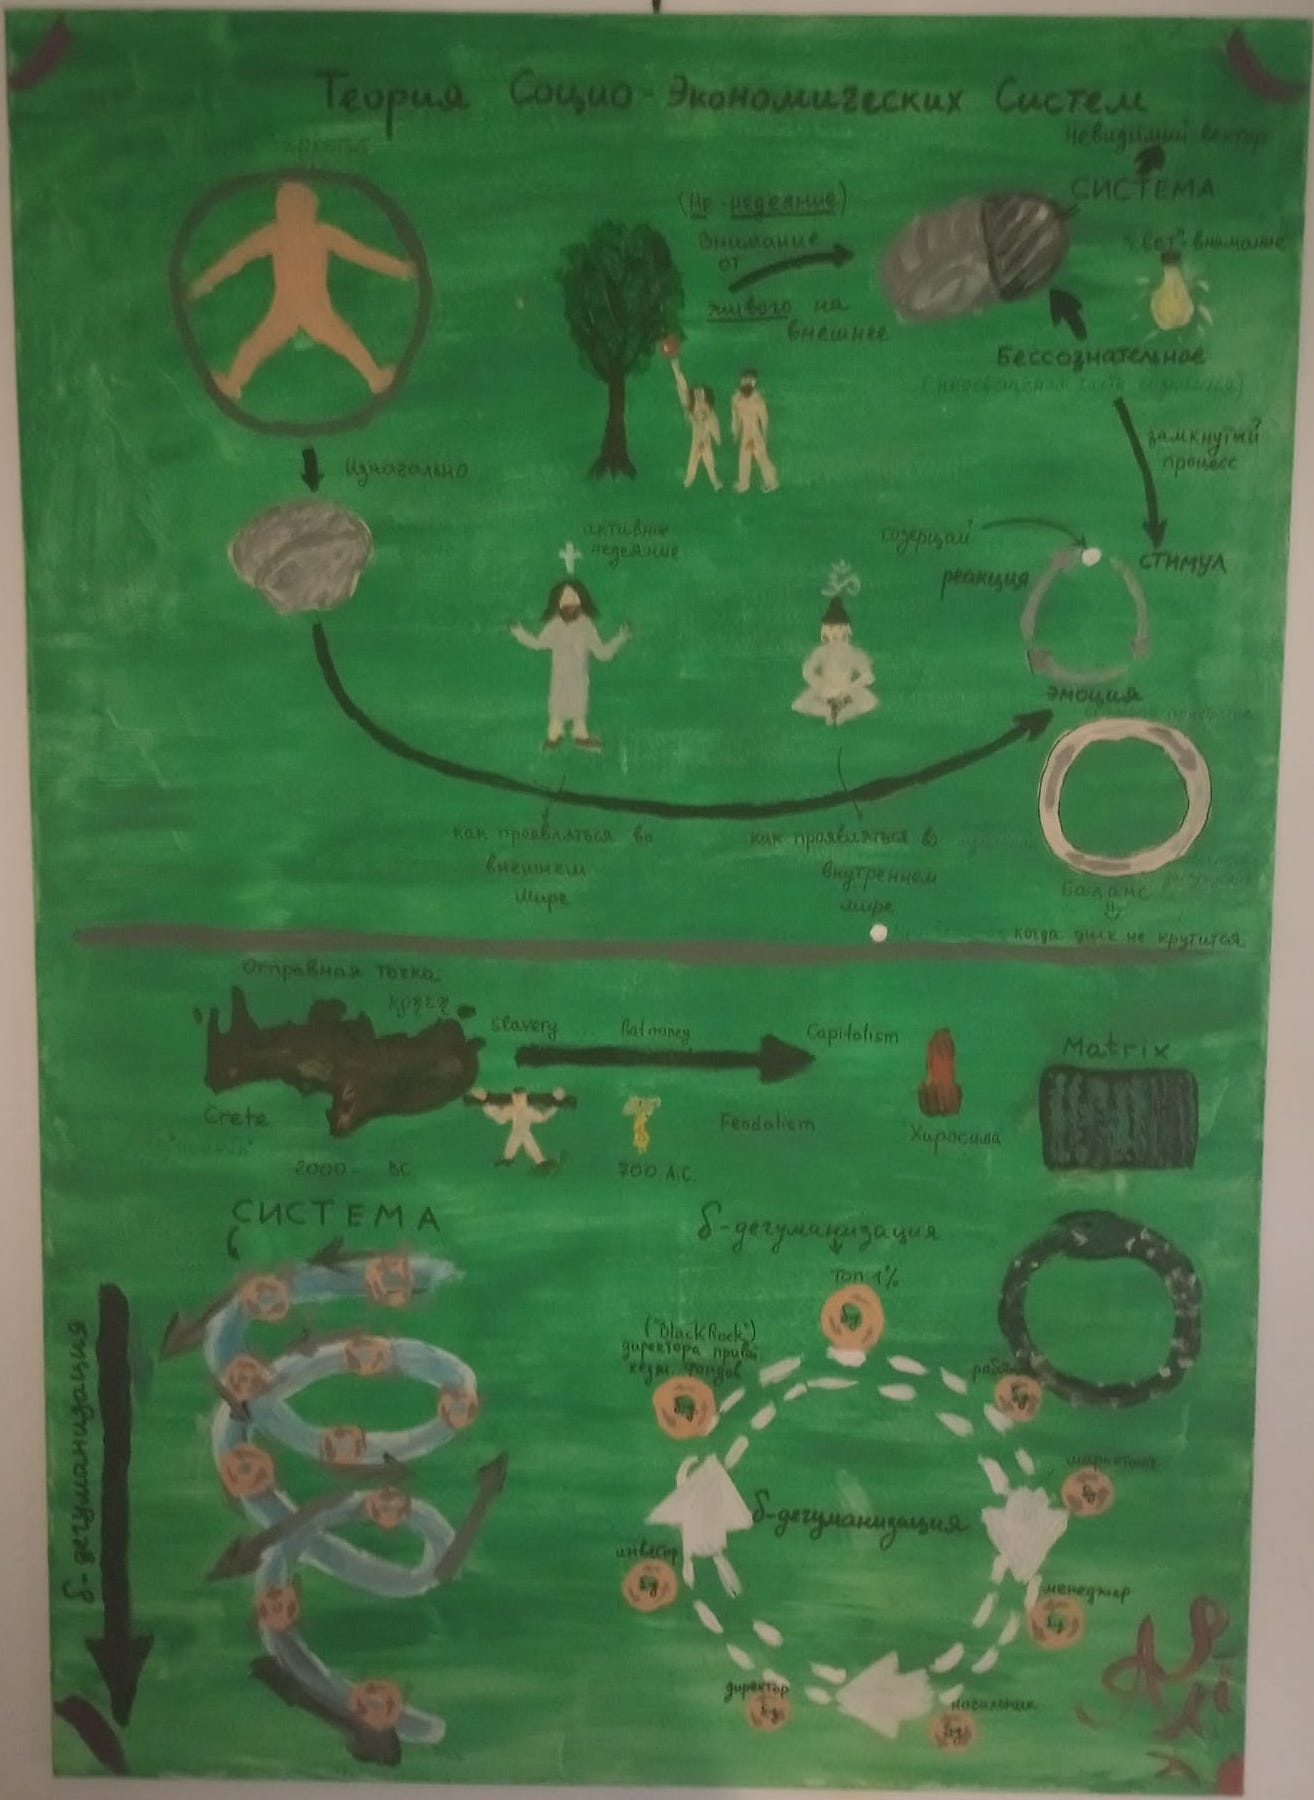
\includegraphics[width=0.95\textwidth]{fig/theory.jpeg}
    \caption{\textbf{Theory of THE \SYSTEM{} --- Complete Visualization}: This illustration shows the emergence of THE \SYSTEM{} from the Fall, its evolution through history, and the dynamics of \deltaDehum{}. \textbf{Upper section:} The origin of the unconscious and the Fall, showing the shift from unity (Vitruvian man in circle) to fragmentation (Adam and Eve, Tree of Knowledge), where attention shifts from ``living/internal'' to ``external'' stimuli, triggering dopamine loops. From this emerges the Collective Unconscious (``invisible circuit'') giving rise to THE \SYSTEM{} with its own ``mind'' (brain) and memory, operating through cycles of STIMULUS $\to$ EMOTION $\to$ REACTION $\to$ EVENT. Christ and Buddha are shown as alternative paths offering ``active non-action'' and ``contemplation of reaction''---paths to consciousness opposing THE \SYSTEM{}'s automated reactions. \textbf{Middle section:} Historical evolution showing different \SES{} manifestations over time---from Crete ($\sim$2000 BCE, close to ``Paradise''), through Slavery, Feudalism, Capitalism, to Hiroshima (symbol of destructive potential), with the Matrix as the ultimate endpoint THE \SYSTEM{} tends toward. \textbf{Lower section:} The spiral of \deltaDehum{}, visualizing the descending trajectory where each iteration of \SES{} accumulates dehumanization, with people (``disks'') rotating under THE \SYSTEM{}'s influence. The exploitation cycle of modern capitalism is shown: Work $\to$ Money (Salary) $\to$ Consumption (Shopping) $\to$ Accumulation (by Top 1\%, BlackRock, etc.) $\to$ Investment (Investor) $\to$ Work, feeding \deltaDehum{} and capital concentration. This visualization successfully conveys how psychological (the Fall, unconscious), social (\SES{}, 1\%/99\% division), and historical (system evolution) levels interconnect in the THE \SYSTEM{} framework.}
    \label{fig:theory}
\end{figure}

\textbf{Upper Section --- The Origin of the Unconscious and the Fall:}
\begin{itemize}
    \item \textbf{Initial State (``Originally''):} A human figure (reminiscent of the Vitruvian Man) enclosed in a circle, symbolizing wholeness and unity.
    \item \textbf{The Fall:} Adam and Eve depicted at the Tree of Knowledge. An arrow indicates the shift of ``attention'' from the ``living/internal'' toward the ``external,'' corresponding to the idea of consciousness moving away from intrinsic value toward external objects and stimuli---the activation of the dopamine loop.
    \item \textbf{Emergence of THE \SYSTEM{}:} From this shift arises the Collective Unconscious (shown as an ``invisible circuit''), from which THE \SYSTEM{} itself emerges, complete with a ``mind'' (``brain'') and ``memory.'' A cycle is illustrated: STIMULUS $\to$ EMOTION $\to$ REACTION $\to$ EVENT, representing a closed loop within the unconscious.
    \item \textbf{Christ and Buddha:} Shown as figures offering alternative paths or responses (``active non-action,'' ``contemplate the reaction''). They represent paths toward awareness that resist the automatic reactions generated by THE \SYSTEM{}.
\end{itemize}

\textbf{Middle Section --- Historical Evolution and THE \SYSTEM{} Manifestations:}
\begin{itemize}
    \item \textbf{Timeline:} Various \SES{} configurations throughout history are shown: Crete ($\sim$2000 BCE) as a starting point (perhaps close to ``Paradise''), followed by Slavery, Feudalism, Capitalism, and Hiroshima (as a symbol of destructive potential). This illustrates the evolution of \SES{} under THE \SYSTEM{}'s influence.
    \item \textbf{The Matrix:} Shown as the endpoint or limit of THE \SYSTEM{}'s evolution---the ultimate state toward which it tends.
\end{itemize}

\textbf{Lower Section --- Mechanisms of THE \SYSTEM{} and \deltaDehum{}:}
\begin{itemize}
    \item \textbf{Spiral of \deltaDehum{}:} Visualized as a descending spiral, where each turn represents an iteration of \SES{} accumulating dehumanization. People (represented as ``disks'') rotate under THE \SYSTEM{}'s influence.
    \item \textbf{Cycle of Exploitation:} A circle illustrating modern capitalism: Work $\to$ Money (Salary) $\to$ Consumption (Shopping) $\to$ Accumulation (by Top 1\%, BlackRock, etc.) $\to$ Investment (Investor) $\to$ Work. This cycle feeds \deltaDehum{} and the concentration of capital.
\end{itemize}

\textbf{Key Observations:}
\begin{itemize}
    \item \textit{Rich in meaning:} The illustration successfully conveys the main ideas of S.V.E.~XII in visual form, showing the interconnection between psychological (the Fall, the unconscious), social (\SES{}, the 1\%/99\% division), and historical (evolution of systems) levels.
    \item \textit{Metaphorical power:} Use of metaphors (spiral, brain of the invisible hand, Matrix) makes complex concepts more accessible.
    \item \textit{Holistic view:} It elegantly shows how different elements of the theory (THE \SYSTEM{}, \deltaDehum{}, the Fall, Christ/Buddha as alternatives) are linked into a unified worldview.
    \item \textit{Educational potential:} This is an excellent visual foundation for explaining THE \SYSTEM{} theory and can be used in presentations, articles, or as a starting point for further discussions.
\end{itemize}

\section{A psychogenesis sketch of ``the Fall''}
\label{app:fall}
From first preference-inversion (valuing ``thing'' over self/other) to dopaminic loops, then extension of ``thing-logic'' to humans (slavery), yielding the conscious/unconscious split as energy-saving under coercion---a metaphorical account of the SYSTEM’s origin. % :contentReference[oaicite:7]{index=7}


\subsection{Foundational Axioms of THE \SYSTEM{}}

We formalize THE \SYSTEM{} through three core axioms:

\begin{axiom}[Fragmentation of Consciousness (A1: Unconscious Primacy)]
\label{ax:fragmentation}
Human consciousness originated in unity but underwent a ``Fall''---a topological event creating a split between conscious awareness (light) and collective unconscious (shadow). This split enables both creativity and systemic distortion. The majority of human behavior is driven by unconscious processes (biases, fears, desires) operating below awareness. Conscious thought is often post-hoc rationalization.
\end{axiom}

\begin{axiom}[Emergent Systemic Intelligence (A2: Socio-Economic Embedding)]
\label{ax:emergence}
Socio-economic systems (\SES{}) emerge from and reinforce unconscious patterns, creating an ``invisible hand'' that guides collective behavior toward self-perpetuation, often at the cost of individual flourishing. Unconscious patterns are shaped, reinforced, and transmitted through socio-economic structures. To change consciousness, we must change \SES{} parameters (П$_1$--П$_5$).
\end{axiom}

\begin{axiom}[Dehumanization Dynamics (A3: Emergent Autonomy)]
\label{ax:dehumanization}
THE \SYSTEM{} accumulates \deltaDehum{}---small, systemic reductions in perceived humanity---through power imbalances, leading to self-reinforcing cycles of inequality and suffering. Once established, THE \SYSTEM{} exhibits quasi-autonomous dynamics, perpetuating itself through feedback loops, institutional capture, and resistance to disruption.
\end{axiom}

\subsection{Operational test for $\delta$-dehumanization}
\label{subsec:delta_test}

Define $\delta$-dehumanization as a baseline economic act one would \emph{not} do to someone they love. Heuristics: (i) grief-exploiting ads targeting children; (ii) knowingly selling defective goods to the unaware. This test provides a practical detector of dehumanizing drift in everyday operations. % :contentReference[oaicite:2]{index=2}

\paragraph{Illustrative responsibility chain (advertising case).}
\begin{enumerate}\itemsep0.2em
\item Marketer optimizes short-term KPIs under deadline pressure;
\item Manager cascades KPI pressure downstream;
\item Directors face status/cost expectations and investor reporting;
\item Meta-investors (``1\%'' risk holders) fear loss of status/power, prefer populace busyness;
\item Workers overworked $\rightarrow$ rely on fast food for kids influenced by ads.
\end{enumerate}
Result: a closed loop where $\delta$ accumulates despite local rationality at each step. % :contentReference[oaicite:3]{index=3}


% Human=Environment×SES×Innate (раздел Env vs SES)
\begin{figure}[h]\centering
\includegraphics[width=0.85\linewidth]{fig/human_as_mosaic_ses_dna.png}
\caption{Human as Environment $\times$ SES $\times$ Innate (mosaic of internalized others).}
\label{fig:human_mosaic}
\end{figure}


\begin{figure}[h]
\centering
\includegraphics[width=0.85\linewidth]{fig/human_evolution_parallel.png}
\caption{Parallel between individual development and collective evolution.}
\label{fig:human_parallel}
\end{figure}

% Humanity-as-teenager (раздел философии будущего)
\begin{figure}[h]\centering
\includegraphics[width=0.8\linewidth]{fig/human_evolution.png}
\caption{Parallel of individual maturation and humanity-as-teenager metaphor.}
\label{fig:human_teen}
\end{figure}



\subsection{\SES{} Parameterization}

We parameterize \SES{} with five dimensions that define how a society organizes resources, incentives, and power:

\begin{parameter}[П$_1$: Core Values \& Incentive Alignment]
\label{par:values}
What the system optimizes for (e.g., money, power, harmony) and the degree to which rewards align individual behavior with collective well-being. Current systems are highly misaligned (rewarding extraction over contribution). PEMY aims for alignment.
\end{parameter}

\begin{parameter}[П$_2$: Motivation Mechanisms \& Resource Distribution]
\label{par:motivation}
How behavior is incentivized (e.g., profit, fear, shared benefit) and the concentration vs. dispersion of wealth/power. Measured by Gini coefficient, wealth ratios. Currently: extreme concentration (top 1\% holds 35\%+ of wealth globally).
\end{parameter}

\begin{parameter}[П$_3$: Information Asymmetry \& Control]
\label{par:information}
Privileged access to information and control of narratives. Manifests as media concentration, algorithmic curation, educational gatekeeping. Creates artificial curvature in the consciousness manifold \CC{}.
\end{parameter}

\begin{parameter}[П$_4$: Social Roles \& Transparency]
\label{par:roles}
Defined hierarchies, identities, and visibility of power structures (e.g., CEO--worker, stakeholder). Degree of transparency and enforcement of ethical accountability. Low transparency grants high freedom to THE \SYSTEM{} operations. PEMY mandates transparency by design.
\end{parameter}

\begin{parameter}[П$_5$: Collective Memory \& Temporal Orientation]
\label{par:memory}
Narratives perpetuating the system (e.g., ``invisible hand'' myth, meritocracy narrative) and the time horizon privileged by incentives (short vs. long term). Current bias: extreme short-termism (quarterly earnings, dopamine hits). Consequences: ecological and social collapse.
\end{parameter}

\begin{figure}[H]
    \centering
    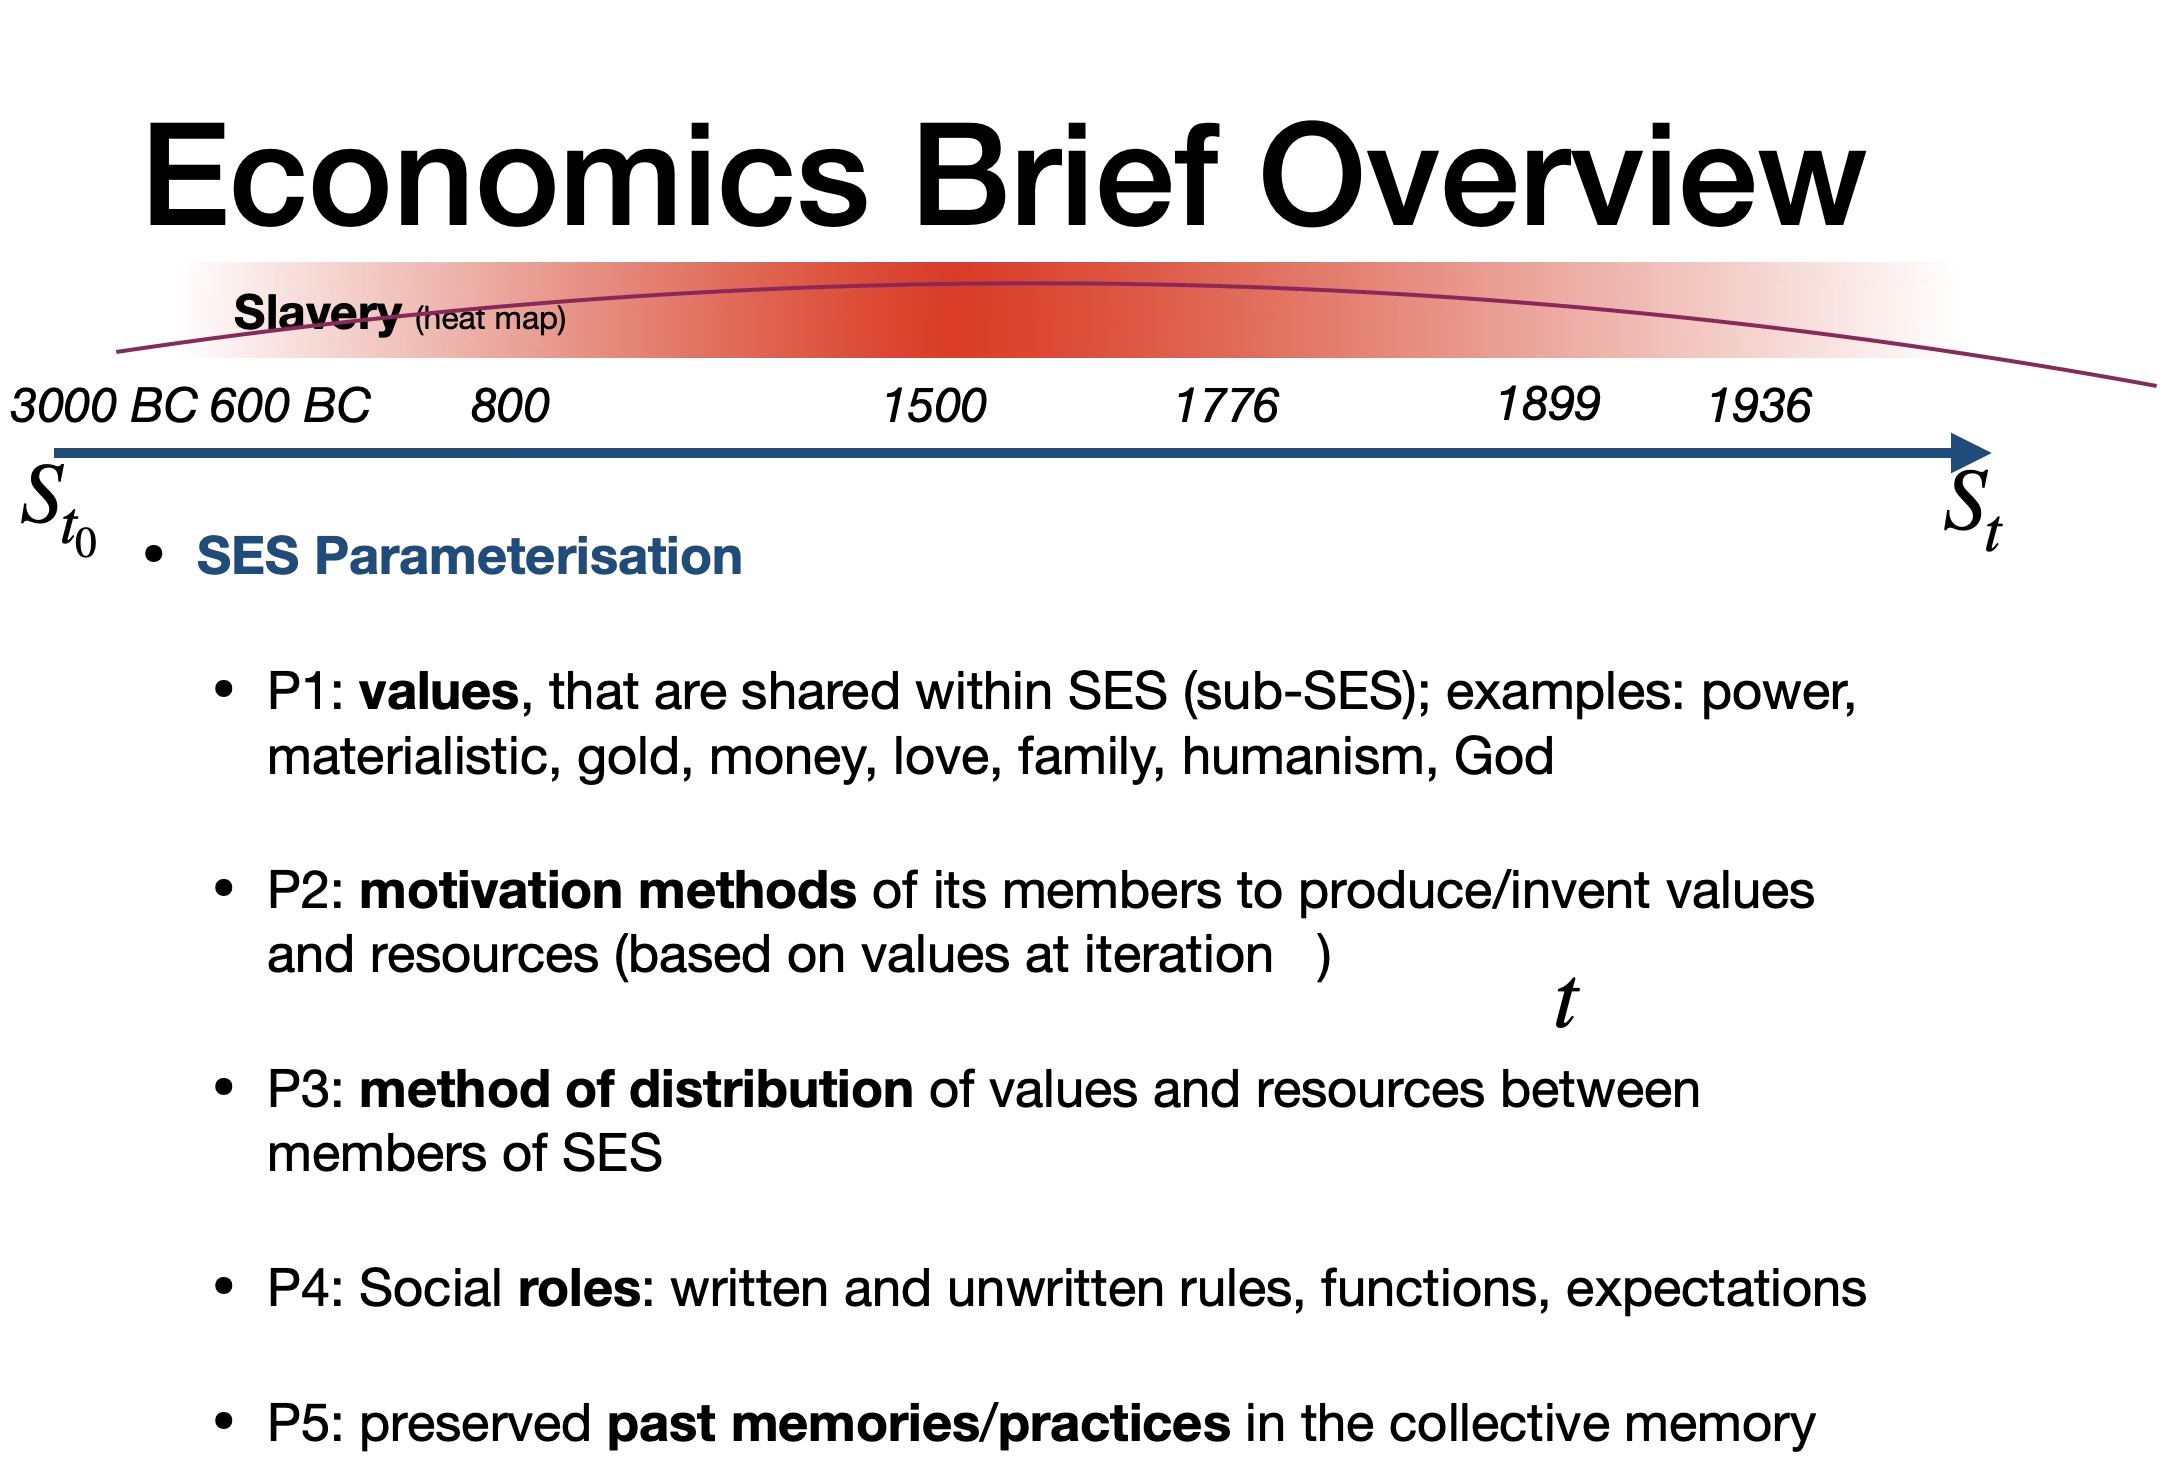
\includegraphics[width=0.85\textwidth]{fig/ses_parameterisation.png}
    \caption{\textbf{\SES{} Parameterization}: Overview of the five parameters (П$_1$--П$_5$) defining socio-economic systems and their evolution across different historical configurations.}
    \label{fig:ses_params}
\end{figure}

\subsection{SYSTEM Parameterization (P1–P5)}
\label{subsec:system_parameterization}

The SYSTEM’s dynamics can be decomposed into five operational levers (P1–P5) that jointly modulate informational exposure, attention allocation, incentive structures, institutional persistence, and psychological conditioning. This parameterization provides actionable handles for diagnosis and intervention.


\begin{table}[h]
\centering
\caption{Operational parameterization of the SYSTEM (P1–P5) with intervention handles.}
\label{tab:system_p_params}
\renewcommand{\arraystretch}{1.12}
\begin{tabularx}{\linewidth}{@{}lXX@{}}
\toprule
\textbf{Param} & \textbf{Description} & \textbf{Example levers / interventions} \\
\midrule
P1 (Information Flow) & Structure and velocity of information diffusion; filtration/agenda-setting. &
Media plurality, open protocols, transparency mandates, friction for virality, algorithmic diversity. \\
P2 (Attention Allocation) & Competition for scarce cognitive resources; salience shaping. &
Time caps, default quiet modes, ad load limits, humane UX, attention dividends to users. \\
P3 (Economic Incentives) & Reward mechanisms driving platforms/actors; monetization vectors. &
Tax/regulatory realignment, public-interest funding, anti-gaming audits, externality pricing. \\
P4 (Institutional Inertia) & Path dependence and lock-in of rules, norms, and infrastructures. &
Sunset clauses, reversible-by-design policy, modular governance, sandboxing reforms. \\
P5 (Psychological Conditioning) & Behavioral scripts, priming, and norm-internalization loops. &
Critical media literacy, deconditioning curricula, choice architecture audits, nudge hygiene. \\
\bottomrule
\end{tabularx}
\end{table}

\begin{table}[h]
\centering
\caption{Indicative metrics/proxies for monitoring P1–P5.}
\label{tab:system_p_metrics}
\renewcommand{\arraystretch}{1.12}
\begin{tabularx}{\linewidth}{@{}lXX@{}}
\toprule
\textbf{Param} & \textbf{Primary proxies} & \textbf{Risk signals} \\
\midrule
P1 & Source entropy, feed diversity index, latency to correction & Echo amplification, rumor half-life \\
P2 & Session length variance, notification rate, dwell-time balance & Attention monoculture, compulsive loops \\
P3 & Revenue mix (ads/subs), externality score, fraud/gaming rate & Perverse incentives, misinfo profitability \\
P4 & Policy half-life, reversal cost, dependency graph density & Irreversibility, brittle cascades \\
P5 & Bias awareness score, dissent survival rate, norm flexibility & Learned helplessness, stigma of critique \\
\bottomrule
\end{tabularx}
\end{table}

\noindent
In the remainder, we reference P1–P5 when analyzing conditioning mechanisms (\S\ref{sec:mechanisms}), education (\S\ref{sec:education}), attention economy (\S\ref{sec:attention}), and self-destructive dynamics (\S\ref{sec:self_destruction}), using Table~\ref{tab:system_p_params} as a compact index of intervention handles.

\begin{table}[h]
\centering
\caption{SES examples via P1--P5 parameterization}
\label{tab:ses_examples}
\renewcommand{\arraystretch}{1.1}
\begin{tabular}{@{}llllll@{}}
\toprule
\textbf{SES} & P1 (values) & P2 (motivation) & P3 (distribution) & P4 (roles) & P5 (memory) \\
\midrule
Slavery & materialism & violence & to owners & slaver/slave & coercive norms \\
Socialism/Communism & equality (decl.) & ideology/labor-days & formal equality & party/worker & state-first \\
\bottomrule
\end{tabular}
\end{table}
% :contentReference[oaicite:12]{index=12}



\subsection{Social Logic: a minimal calculus for systemic inference}
\label{subsec:social_logic}

\begin{definition}[Social Logic]
A rule-based inference over social phenomena: from observed laws $L_i$ and empirical precedents $(A\!\to\!B,\,B\!\to\!C)$ infer $A\!\to\!C$ for comparable contexts; used to reason about hidden drivers when controlled experiments are infeasible. % :contentReference[oaicite:3]{index=3}
\end{definition}

\paragraph{Indicative laws (non-exhaustive).}
L1: psychological projection; L2: “greener grass” effect; L3: strategy copying; L4: boiled-frog value drift; L5: desire depends on self-awareness. These enable reconstructive arguments (e.g., Minoan case) when direct evidence is sparse. % :contentReference[oaicite:4]{index=4}



\subsection{Elites as Hostages of THE \SYSTEM{}}

A crucial insight: even elites are ``hostages'' of THE \SYSTEM{}. As emerged from dialogues, the average person raised in elite conditions would likely adopt similar behaviors. This systemic trap shifts blame from individuals to structures, emphasizing empathy and awakening for all levels of society.

\textbf{Psychological Traps for Elites:}
\begin{itemize}
    \item \textbf{Fear of Loss:} Losing status, wealth, or power activates deep survival mechanisms
    \item \textbf{Value Inconsistencies:} Public statements vs. actual behaviors (see Figure~\ref{fig:zuck_inconsistency} on Zuckerberg's posts illustrating goal--reality gaps)
    \item \textbf{Stockholm Syndrome:} Psychological identification with THE \SYSTEM{} itself
    \item \textbf{Cognitive Dissonance:} Justifying extractive practices through meritocracy narratives
    \item \textbf{Isolation:} Living in ``bubbles'' disconnected from consequences of policies
\end{itemize}

\textbf{Proposals for Elite Awakening:}
\begin{itemize}
    \item \textbf{``Experience of Consequences'' Programs:} Elites spend time living under conditions their policies create (e.g., minimum wage, no healthcare)
    \item \textbf{Transparency Requirements:} Mandatory disclosure of wealth sources, influence networks
    \item \textbf{Multi-Capital Accounting:} Measuring success beyond financial metrics
    \item \textbf{Cognitive OS Training:} S.V.E.~X protocols for systemic awareness
    \item \textbf{Facilitated Dialogue:} Between elites and those affected by their decisions
\end{itemize}

This framework integrates with Axiom~\ref{ax:dehumanization}, highlighting THE \SYSTEM{}'s fractal influence across all societal levels---from the homeless to billionaires, all are trapped in patterns larger than themselves.

\begin{figure}[H]
    \centering
    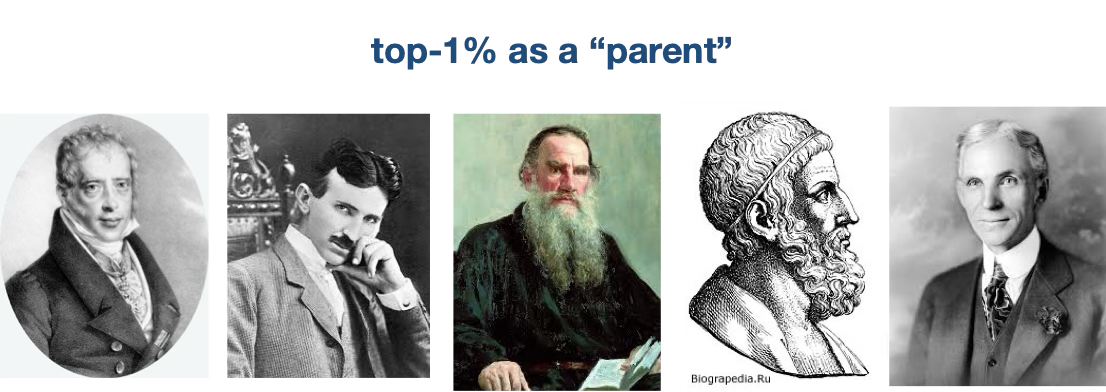
\includegraphics[width=0.75\textwidth]{fig/top1percent_as_Parent_for_Humanity.png}
    \caption{\textbf{Top 1\% as ``Parents'' for Humanity}: Illustration showing how influential figures (elites) function as symbolic ``parents'' within the THE \SYSTEM{} framework, shaping collective norms and values while simultaneously being constrained by the very system they perpetuate.}
    \label{fig:top1percent}
\end{figure}

\begin{figure}[h]
\centering
\includegraphics[width=0.8\linewidth]{fig/parent_top1_percent.png}
\caption{The metaphorical ``parent'' (top 1\%) in the global family model.}
\label{fig:parent_one_percent}
\end{figure}

% 1% as “parents” (раздел про элиты/1%)
\begin{figure}[h]\centering
\includegraphics[width=0.85\linewidth]{fig/parents_top1percent.png}
\caption{Top 1\% as metaphorical “parents” of humanity.}
\label{fig:top1_parents}
\end{figure}



\begin{figure}[h]
\centering
\includegraphics[width=0.8\linewidth]{fig/ses_fractals.png}
\caption{Fractal nature of the SYSTEM — repeating control and conditioning patterns across scales.}
\label{fig:fractals}
\end{figure}


\newpage

\section{Theoretical Foundations}
\label{sec:theory}

This section outlines the conceptual lineage of the SYSTEM framework by integrating key insights from Jung, Smith, and Plato. Each provides a distinct dimension: the psychological (Jung), the socio-economic (Smith), and the philosophical-metaphysical (Plato). Together, they form the triadic foundation of the SYSTEM's dynamics.

\vspace{0.5em}
\noindent
Beyond the triadic synthesis of Jung, Smith, and Plato, the SYSTEM can be parameterized through five operational levers (P1–P5) defining its dynamics. These parameters encapsulate informational flow, attention allocation, economic incentives, institutional inertia, and psychological conditioning. Understanding their interrelations allows for both diagnosis and potential systemic intervention.

\begin{figure}[h]
\centering
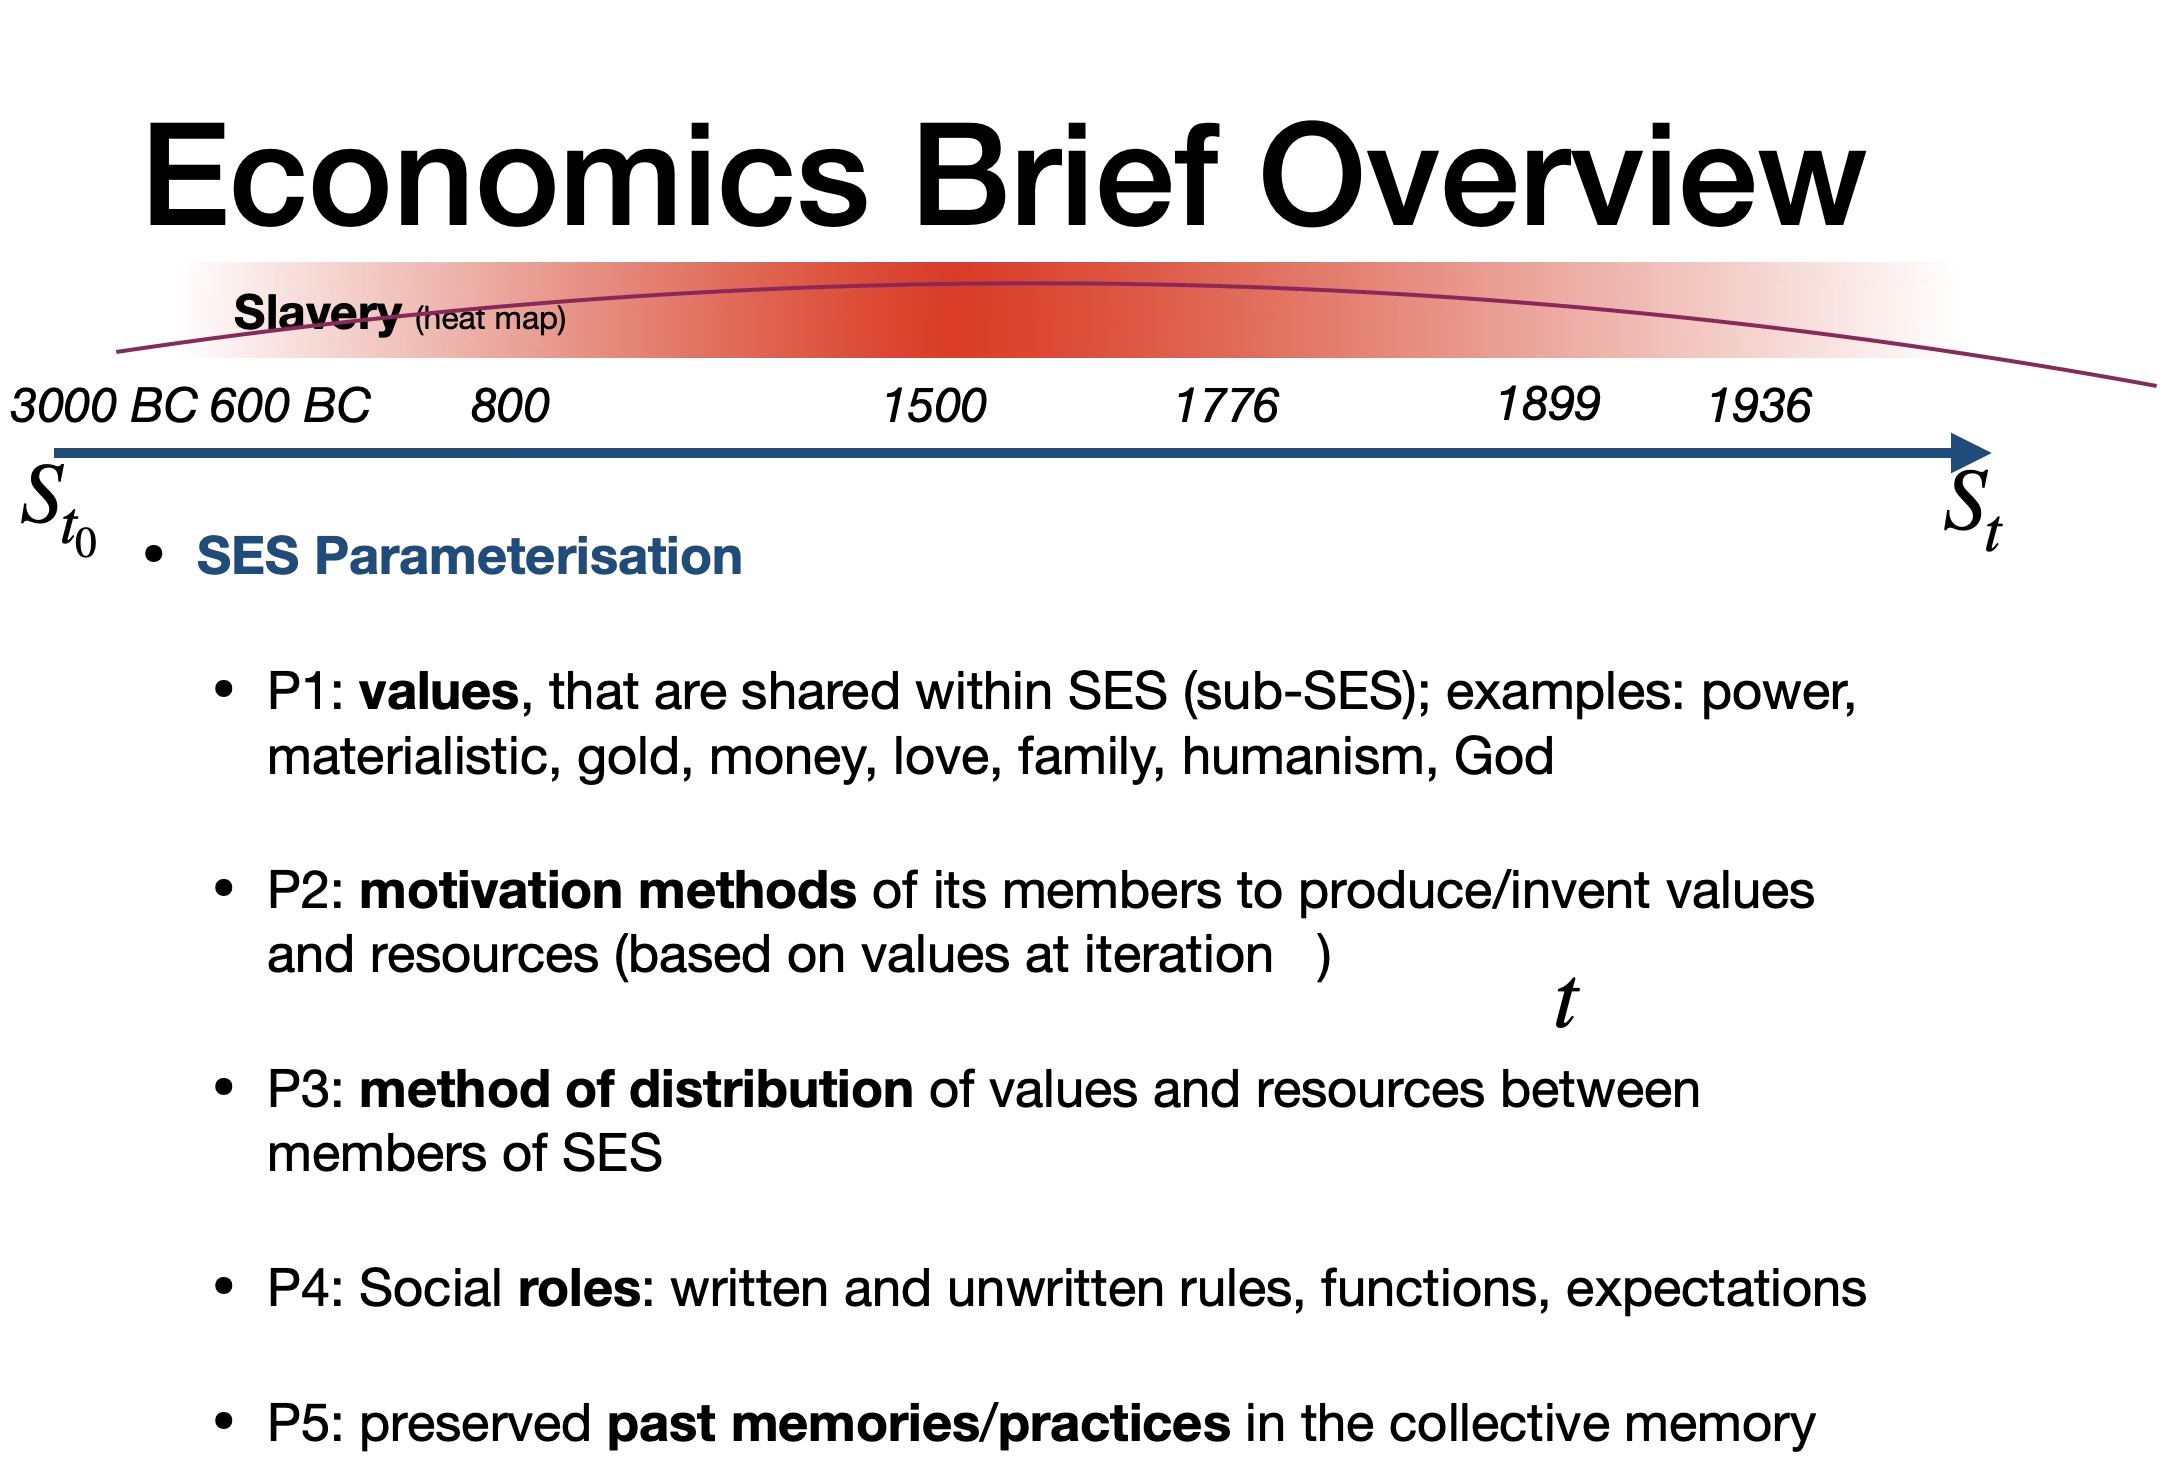
\includegraphics[width=0.9\linewidth]{fig/ses_parameterisation.png}
\caption{Parameterization of the SYSTEM through five core levers (P1–P5) representing informational, economic, institutional, and psychological control dimensions.}
\label{fig:ses_parameterisation}
\end{figure}


\subsection{Jungian Dimension: The Shadow and Individuation}
Carl Jung’s model of the psyche provides a psychological substrate for understanding SYSTEM behavior. The archetypal "Shadow" mirrors the SYSTEM’s repressed collective impulses, while individuation parallels the process of awakening from systemic conditioning.

\begin{table}[h]
\centering
\caption{Mapping Jungian Concepts to SYSTEM Dynamics}
\label{tab:jung_mapping}
\begin{tabular}{|l|l|}
\hline
\textbf{Jungian Concept} & \textbf{SYSTEM Interpretation} \\ \hline
Archetypes & Collective behavioral templates shaping social roles \\ \hline
Shadow & Suppressed collective impulses projected onto “others” \\ \hline
Persona & Social masks sustaining systemic harmony \\ \hline
Individuation & Process of deconditioning and systemic transcendence \\ \hline
Collective Unconscious & Shared cognitive substrate exploited by media and ideology \\ \hline
\end{tabular}
\end{table}

\subsection{Mosaic selves and nations as sub-personalities}
\label{subsec:mosaic_nations}

An individual is a mosaic of internalized interactions; by analogy, nations can be modeled as sub-personalities of humanity. Psychoanalytic tooling thus scales to geopolitics, interpreting conflicts as intra-psychic dynamics at a civilizational level. % :contentReference[oaicite:4]{index=4}



\subsection{Smithian Dimension: The Invisible Hand and Systemic Self-Regulation}
Adam Smith’s metaphor of the "invisible hand" offers an early precursor of systemic autonomy. Within the SYSTEM, this mechanism mutates from a market equilibrium to a feedback loop maintaining collective illusions of order and progress.

\subsection{Platonic Dimension: From the Cave to the Matrix}
Plato’s allegory of the Cave encapsulates the epistemic entrapment central to the SYSTEM. The shadows on the cave wall correspond to mediated realities—images and narratives shaping collective consciousness.

The synthesis of these three perspectives yields a multidimensional model of systemic conditioning: psychological, economic, and metaphysical.

\begin{table}[h]
\centering
\caption{Mapping Plato’s Cave Allegory to SYSTEM Constructs}
\label{tab:plato_mapping}
\begin{tabular}{|l|l|}
\hline
\textbf{Element in the Cave} & \textbf{SYSTEM Interpretation} \\ \hline
Prisoners & Conditioned individuals within societal frameworks \\ \hline
Chains & Ideological, educational, and media conditioning \\ \hline
Shadows & Mass media representations and digital simulations \\ \hline
Fire & The limited energy source of collective attention \\ \hline
Outside World & Unmediated perception / awakening consciousness \\ \hline
Return to Cave & Resistance to systemic awakening and social reintegration \\ \hline
\end{tabular}
\end{table}

\subsection{Environment vs. Socio-Economic Systems (SES)}
\label{subsec:env_vs_ses}

We distinguish natural \emph{Environment} from human-made \emph{Socio-Economic Systems (SES)}. A person can be modeled as
\[
\textbf{Human} = \textbf{Environment} \times \textbf{SES} \times \textbf{Innate}.
\]
Conflating Environment and SES obscures which factor drives outcomes; separating them clarifies that many pathologies are \emph{system-made}, not “natural”. % :contentReference[oaicite:0]{index=0}

\begin{table}[h]
\centering
\caption{Environment vs. SES: distinct influences}
\label{tab:env_ses_split}
\begin{tabular}{|l|p{0.68\linewidth}|}
\hline
\textbf{Environment} & Climate, seasons, biomes, ecosystems; persists without humans. \\
\hline
\textbf{SES} & Formal/informal rules of human interaction (markets, firms, schools, prisons, states); artifacts of collective values. \\
\hline
\end{tabular}
\end{table}

\subsection{Balanced and Flexible SES}
\label{subsec:balanced_flexible_ses}

\begin{definition}[Balanced SES]
A socio-economic system is \emph{balanced} if an arbitrary participant can satisfy basic physical, emotional, and social needs starting from \emph{any} admissible role within a finite number of iterations of the system's normal operation. % :contentReference[oaicite:0]{index=0}
\end{definition}

\begin{definition}[Flexible SES]
A socio-economic system is \emph{flexible} if role transition is feasible for an arbitrary participant within a finite number of system iterations without irreversible loss of agency or dignity. % :contentReference[oaicite:1]{index=1}
\end{definition}

\noindent These properties provide evaluation criteria and reform targets (cf. P1--P5 levers in Table~\ref{tab:system_p_params}). % :contentReference[oaicite:2]{index=2}


\newpage

% ==================== PART II ====================
\section{Part II: Geometry of the Fall}

\subsection{The Consciousness Manifold \CC{}}

We model collective consciousness as a Riemannian manifold \CC{}, where points represent states of awareness---both individual and collective. The \Fall{} introduces curvature into this manifold, making paths toward love (\Love{}) and unity geometrically longer, while suffering (\Suffering{}) geodesics become ``efficient'' default trajectories.

\begin{definition}[Consciousness Manifold]
Let \CC{} be a smooth manifold representing the space of possible conscious states. A metric $g$ on \CC{} encodes the ``cost'' or ``difficulty'' of transitioning between states. The Fall introduces curvature: $R \neq 0$ where $R$ is the Riemann curvature tensor.
\end{definition}

\begin{proposition}[Fall Distortion]
\label{prop:fall_distortion}
The \Fall{} maps a flat (or minimally curved) manifold $\mathcal{C}_0$ to one with positive curvature in shadow regions, creating:
\begin{enumerate}
    \item \textbf{Geodesic deviation:} Paths toward \Love{} become longer than paths toward \Suffering{}
    \item \textbf{Trapped states:} Local minima in awareness space (comfort zones, echo chambers)
    \item \textbf{Fragmentation:} Disconnected components (``us vs. them'' thinking)
\end{enumerate}
Formally, if $\gamma_{\LL}(t)$ is a love-oriented path and $\gamma_{\SScri}(t)$ a suffering-oriented path between the same start and end points, then:
\[
\text{Length}(\gamma_{\LL}) > \text{Length}(\gamma_{\SScri})
\]
in the post-Fall metric.
\end{proposition}

\begin{figure}[H]
    \centering
    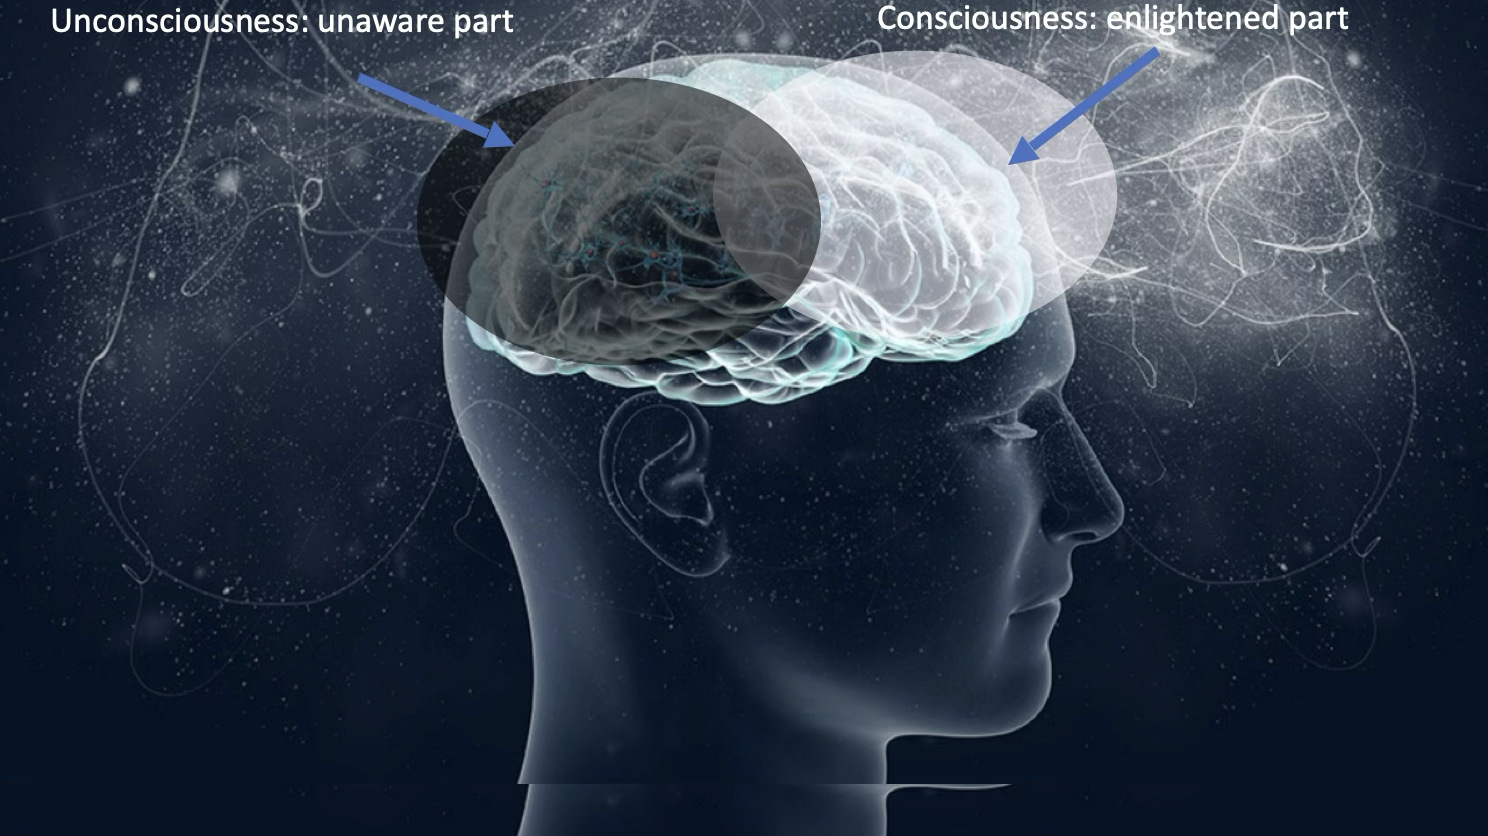
\includegraphics[width=0.75\textwidth]{fig/conciousness_subconciousness_model_eng.png}
    \caption{\textbf{Consciousness and Subconsciousness Model}: The ``light'' of conscious attention illuminates only a small portion of the vast unconscious terrain (shadow). Most of our behavior is driven by patterns in the shadow, which THE \SYSTEM{} exploits.}
    \label{fig:consciousness_model}
\end{figure}

\begin{figure}[h]
\centering
\includegraphics[width=0.9\linewidth]{fig/model_conciousness_subconciousness.pdf}
\caption{Alternative visualization of conscious and subconscious interaction layers.}
\label{fig:conciousness_alt}
\end{figure}


\subsection{Mathematical Formalism of the Fall}

The Fall can be understood as a \textit{phase transition} in the collective consciousness, analogous to symmetry breaking in physics.

\begin{definition}[Pre-Fall State]
Let $\mathcal{C}_0$ represent the pre-Fall consciousness manifold with metric $g_0$. Assume $\mathcal{C}_0$ is flat or has minimal curvature:
\[
R_{ijkl}(g_0) \approx 0
\]
In this state, all paths toward growth (love, unity, awareness) are approximately geodesics---natural and effortless.
\end{definition}

\subsection{Wave propagation of the Fall}
\label{subsec:fall_wave}

Let $\psi(\mathbf{x},t)$ denote collective-consciousness waves; a “Fall” event acts as an impulse shaping boundary conditions via SES, producing traveling/standing modes that imprint $\beta$-dehumanization patterns across societies with lags. Historically isolated cultures (e.g., Minoans) may exhibit delayed coupling. % :contentReference[oaicite:10]{index=10}


\begin{figure}[h]
\centering
\begin{tikzpicture}[scale=1]
\draw (0,0) circle (1.8); % person as balanced circle
\draw[-{Latex[length=3mm]}] (0,0) -- (1.4,0.5) node[anchor=west]{\small SYSTEM vector};
\draw[-{Latex[length=3mm]}] (0,0) -- (-1.2,1.1);
\draw[-{Latex[length=3mm]}] (0,0) -- (-0.5,-1.5);
\node at (0,-2.2) {\small Vectors attempt to torque attention off-balance};
\end{tikzpicture}
\caption{Collective vectors (THE \SYSTEM{}) torque the person’s attention-circle into non-eudaimonic states.} % :contentReference[oaicite:11]{index=11}
\label{fig:vector_torque}
\end{figure}


\begin{definition}[Post-Fall State]
After the Fall, the metric transforms: $g_0 \to g_F$ where $g_F$ encodes the distortions introduced by:
\begin{itemize}
    \item \textbf{Dopamine hijacking:} External stimuli become artificially attractive
    \item \textbf{Trauma imprints:} Past suffering creates ``gravitational wells''
    \item \textbf{Illusion fixation:} Mistaking shadows for reality (Plato's Cave)
    \item \textbf{Fragmentation:} Loss of connection to wholeness
\end{itemize}
The curvature becomes significant: $R_{ijkl}(g_F) \neq 0$.
\end{definition}

\begin{remark}[Christ-Vector as Geodesic]
In \cite{sve4}, the Christ-Vector is defined as the optimal ethical path. In this framework, it corresponds to a geodesic in the \textit{original} flat metric $g_0$, which in the curved post-Fall metric $g_F$ appears as a challenging, non-obvious path requiring conscious effort (``taking up one's cross'').
\end{remark}

\subsection{Historical Evolution of \SES{}}

Figure~\ref{fig:ses_evolution} illustrates how \SES{} parameters have evolved over time, with each historical configuration amplifying certain aspects of inequality and dehumanization:

\begin{figure}[H]
    \centering
    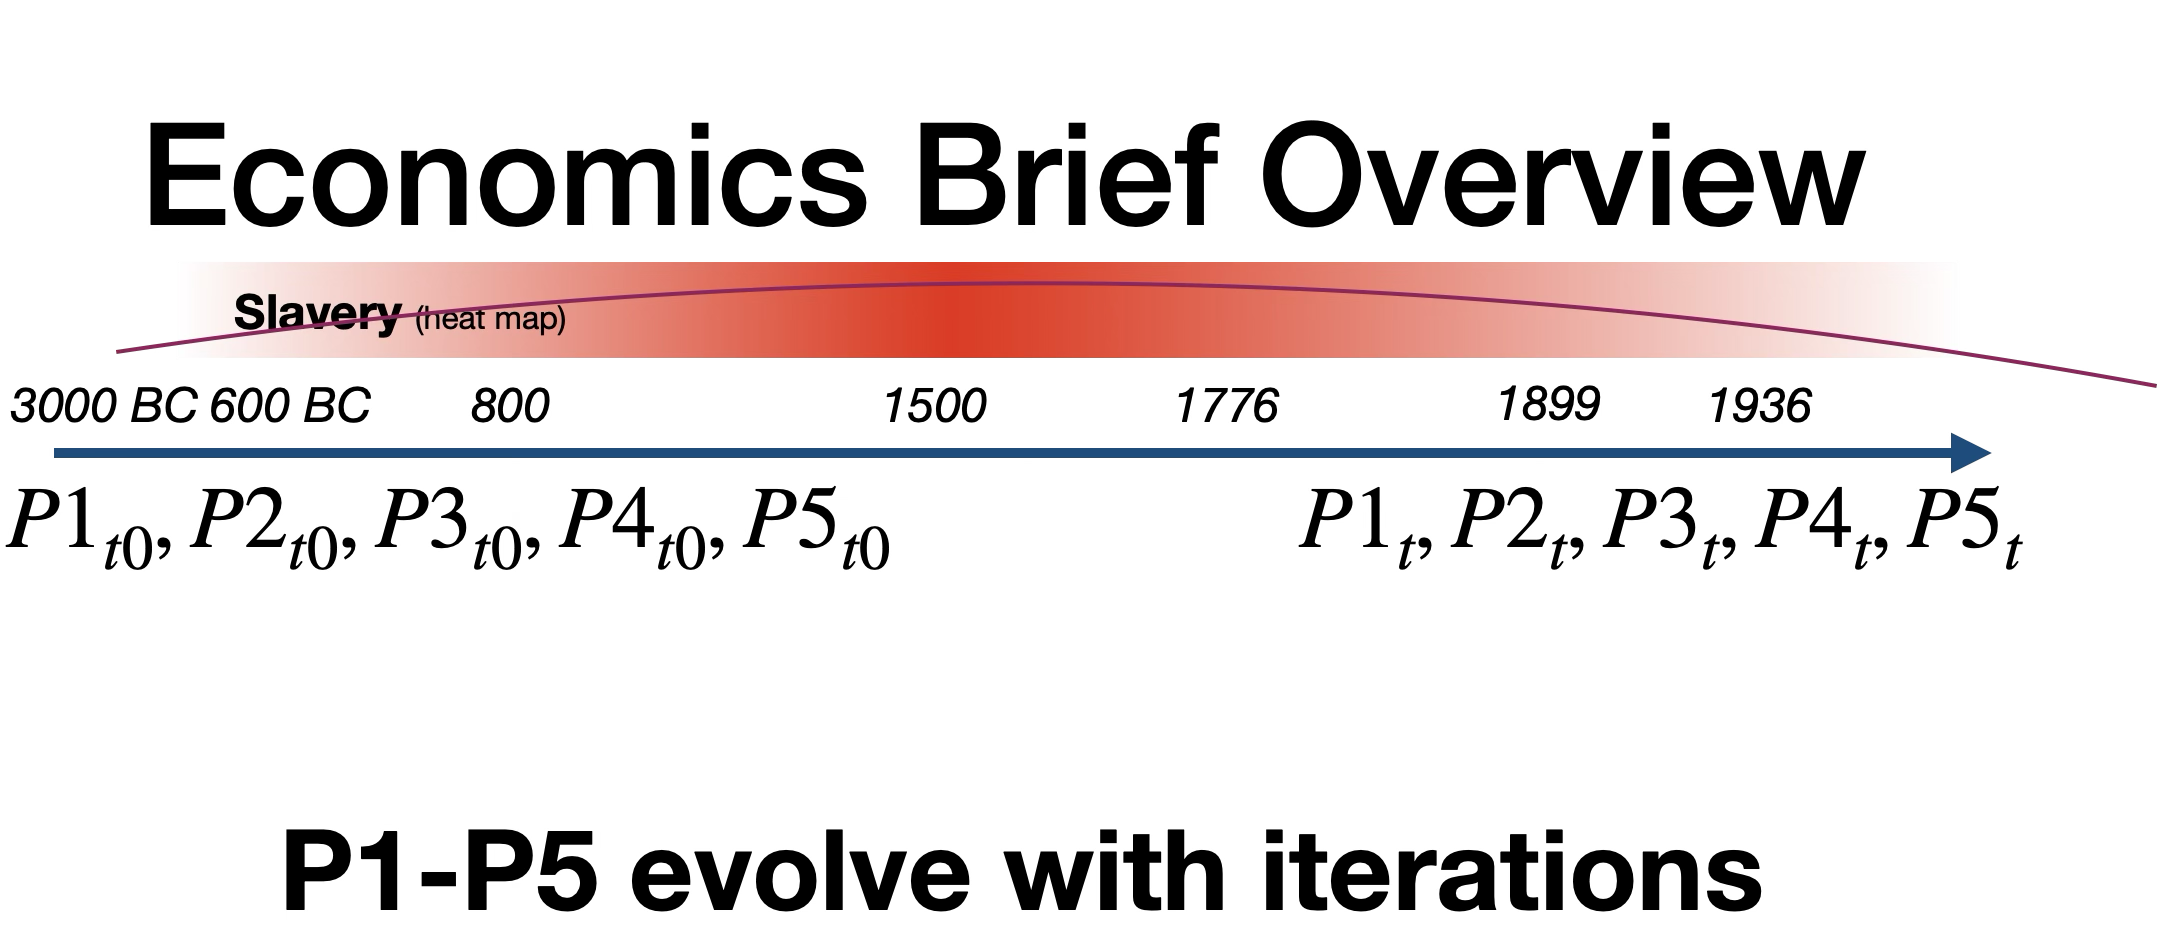
\includegraphics[width=0.85\textwidth]{fig/ses_params_evolution.png}
    \caption{\textbf{Historical Evolution of \SES{} Parameters}: From pre-Fall unity through slavery, feudalism, capitalism, toward the Matrix endpoint. Each transition modifies parameters П$_1$--П$_5$, generally increasing concentration of power and accelerating \deltaDehum{}.}
    \label{fig:ses_evolution}
\end{figure}

\textbf{Key Evolutionary Stages:}

\begin{enumerate}
    \item \textbf{Pre-Fall / Minoan Crete ($\sim$2000 BCE):} Relatively egalitarian, nature-integrated \cite{minoan_crete}
    \begin{itemize}
        \item П$_1$: Harmony, community
        \item П$_2$: Shared resources
        \item П$_3$: Low information control
        \item П$_4$: Fluid social roles
        \item П$_5$: Cyclical time, connection to nature
    \end{itemize}
    
    \item \textbf{Slavery:} Extreme dehumanization codified
    \begin{itemize}
        \item П$_1$: Material extraction, power
        \item П$_2$: Violence, coercion
        \item П$_3$: Total control over enslaved
        \item П$_4$: Master--slave binary
        \item П$_5$: Normalized ownership of humans
    \end{itemize}
    
    \item \textbf{Feudalism:} Hereditary hierarchy
    \begin{itemize}
        \item П$_1$: Land, honor, divine right
        \item П$_2$: Obligation, fealty
        \item П$_3$: Church and nobility monopoly on literacy
        \item П$_4$: King--noble--serf hierarchy
        \item П$_5$: Divine right narrative
    \end{itemize}
    
    \item \textbf{Capitalism:} Abstracted exploitation
    \begin{itemize}
        \item П$_1$: Money, infinite growth
        \item П$_2$: Profit maximization, competition
        \item П$_3$: Media, algorithm control
        \item П$_4$: Owner--worker (CEO--employee)
        \item П$_5$: Invisible hand myth, meritocracy
    \end{itemize}
    
    \item \textbf{Digital Capitalism (Current):} Accelerated extraction
    \begin{itemize}
        \item П$_1$: Data, attention, engagement
        \item П$_2$: Dopamine loops, addiction
        \item П$_3$: Algorithmic curation, filter bubbles
        \item П$_4$: Platform--user asymmetry
        \item П$_5$: ``Free'' services narrative, FOMO culture
    \end{itemize}
    
    \item \textbf{Matrix (Projected Endpoint):} Total capture
    \begin{itemize}
        \item П$_1$: System survival, control
        \item П$_2$: Automated compliance
        \item П$_3$: Complete surveillance, reality control
        \item П$_4$: Human--machine hierarchy
        \item П$_5$: Simulated reality as norm
    \end{itemize}
\end{enumerate}

\subsection{Digitization and the Acceleration of Inequality}

\begin{figure}[h]
\centering
\includegraphics[width=0.9\linewidth]{fig/digitization_pump.png}
\caption{Digitization as a pump shifting value from ``80\%'' to ``top-20\%''.}
\label{fig:digitization_pump}
\end{figure}


The digital era represents a qualitative shift in THE \SYSTEM{}'s operation. Digitization enables:

\begin{itemize}
    \item \textbf{Value Pumping:} Automated extraction of attention, data, and behavioral surplus
    \item \textbf{Winner-Take-All Dynamics:} Network effects concentrate power in platform monopolies
    \item \textbf{Algorithmic Amplification:} AI optimizes for engagement, not wellbeing
    \item \textbf{Surveillance Capitalism:} Every action becomes monetizable data
    \item \textbf{Manufactured Desire:} Precision-targeted manipulation
\end{itemize}

\begin{figure}[H]
    \centering
    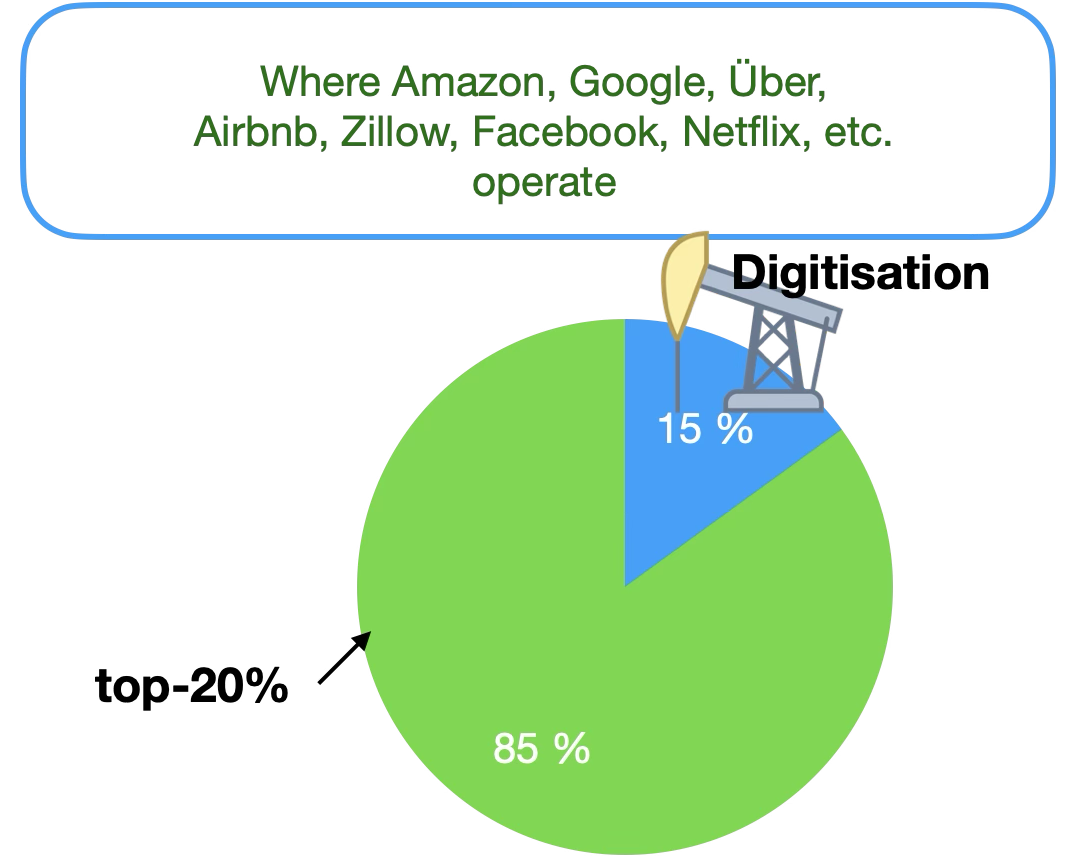
\includegraphics[width=0.75\textwidth]{fig/digitization_and_inequality_pumping_value.png}
    \caption{\textbf{Digitization and Inequality --- Value Pumping}: Illustration showing how digital platforms extract value from users (attention, data, behavioral surplus) and concentrate it upward, accelerating wealth inequality. The ``pump'' metaphor captures the automated, continuous nature of this extraction.}
    \label{fig:digitization_inequality}
\end{figure}

\begin{remark}[The 1971 Inflection Point]
As shown in inequality data (Figure~\ref{fig:inequality}), a sharp divergence occurred around 1971 when the Bretton Woods system collapsed and money decoupled from gold \cite{brettonwoods1971}. This enabled unlimited expansion of debt and financialization, accelerating wealth concentration.
\end{remark}

\newpage

% ==================== PART III ====================
\section{Part III: Empirical Illustrations and Evidence}

\subsection{Inequality Dynamics: The \$50 Trillion Transfer}

Recent analysis reveals that approximately \$50 trillion has been transferred from the bottom 90\% to the top 1\% in the United States alone over the past four decades. This is not incidental---it is the predictable outcome of \SES{} parameter settings under current capitalism.

\begin{figure}[H]
    \centering
    \includegraphics[width=0.75\textwidth]{fig/inequality.png}
    \caption{\textbf{Inequality Growth Over Time}: Data showing the dramatic divergence between productivity and wages starting in the 1970s, and the concentration of wealth in the top 1\%. Sources include Wikipedia and economic research institutes. The 1971 inflection point (end of Bretton Woods) is clearly visible.}
    \label{fig:inequality}
\end{figure}

\subsection{What is Money? --- Functional Analysis}

Money is not a neutral medium of exchange. Within the THE \SYSTEM{} framework, money functions as:

\begin{enumerate}
    \item \textbf{Control Mechanism:} Access to resources, mobility, healthcare, education
    \item \textbf{Energy Token:} Stored human labor and potential
    \item \textbf{Permission System:} What you are allowed to do/be
    \item \textbf{Social Ranking:} Marker of worth in current \SES{}
    \item \textbf{Attention Director:} What gets funded gets done
\end{enumerate}

\begin{figure}[H]
    \centering
    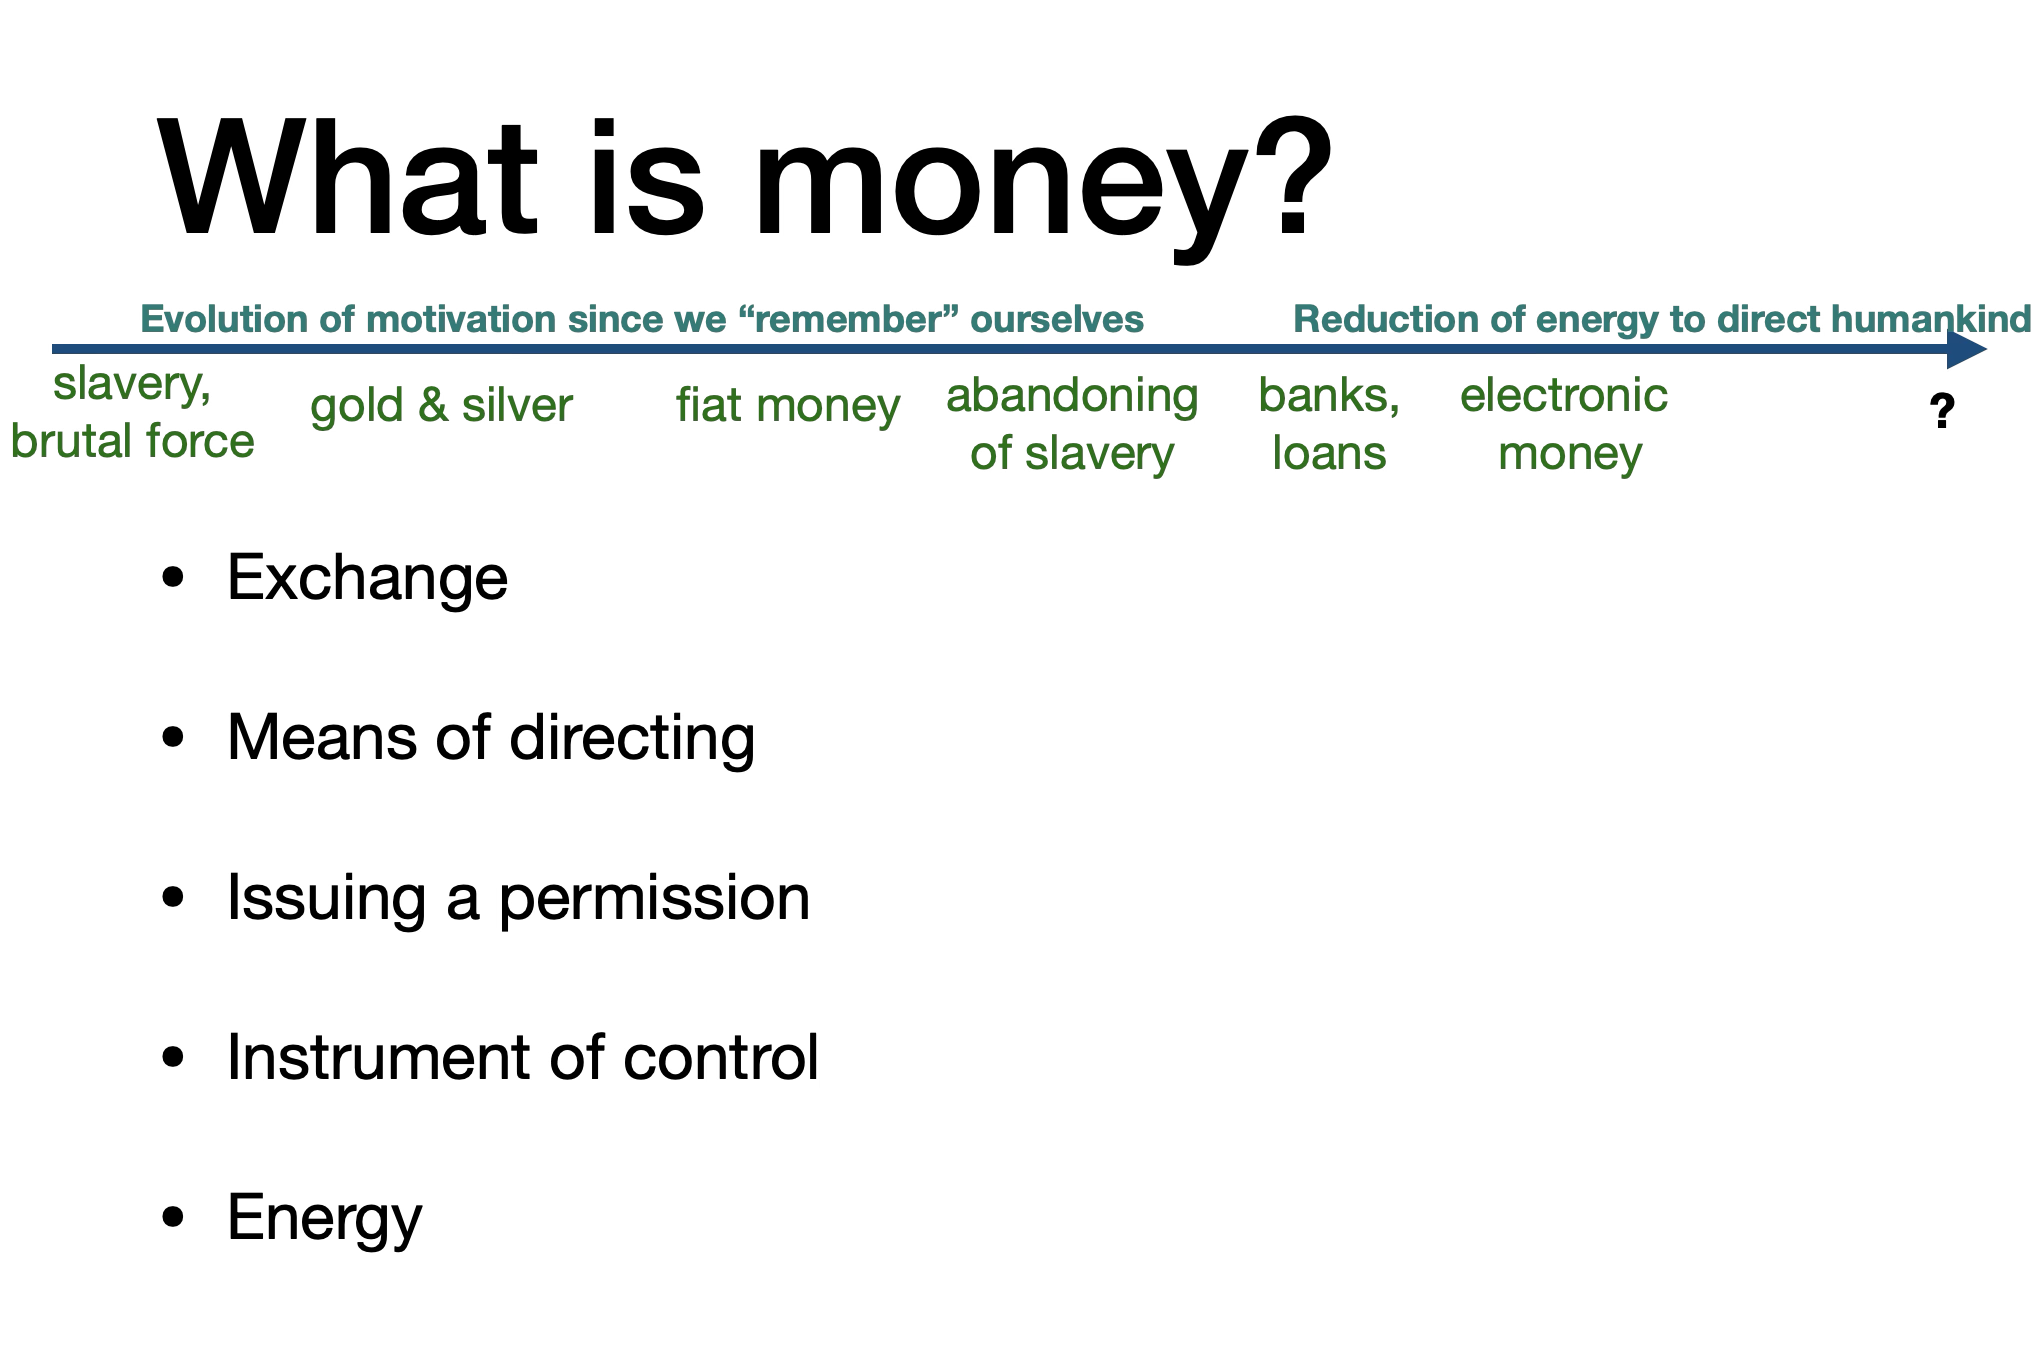
\includegraphics[width=0.75\textwidth]{fig/what_is_money.png}
    \caption{\textbf{What is Money?} (Russian illustration): Conceptual diagram showing money as exchange medium, permission system, control mechanism, and stored energy. Understanding money's multifaceted nature is crucial for seeing how THE \SYSTEM{} operates.}
    \label{fig:money}
\end{figure}

When money becomes the primary value (П$_1$), all other values become instrumentalized. Human relationships, nature, truth itself---all are reduced to economic transactions.

\subsection{Stanford Prison Experiment: \deltaDehum{} in Action}

The Stanford Prison Experiment (SPE) \cite{spe1973} provides a powerful illustration of \deltaDehum{} dynamics. Ordinary college students, randomly assigned to ``guard'' or ``prisoner'' roles, rapidly descended into abusive patterns within days.

\textbf{Key Observations:}
\begin{itemize}
    \item \textbf{Role Capture:} Participants internalized their assigned roles
    \item \textbf{\deltaDehum{} Accumulation:} Small acts of dehumanization escalated
    \item \textbf{Systemic Reinforcement:} Structure enabled and encouraged abuse
    \item \textbf{Normalization:} Participants rationalized increasingly extreme behavior
    \item \textbf{Bystander Effect:} Those not directly involved failed to intervene
\end{itemize}

\begin{figure}[H]
    \centering
    \includegraphics[width=0.75\textwidth]{fig/prison_experiment_illustration_delta_dehumanisation_dynamics.png}
    \caption{\textbf{Stanford Prison Experiment --- \deltaDehum{} Dynamics}: Visualization of how small acts of dehumanization ($\delta$) accumulate over iterations, creating a self-reinforcing cycle. Guards dehumanize prisoners $\to$ prisoners resist or break down $\to$ guards escalate $\to$ further dehumanization. The system structure enables and accelerates this process.}
    \label{fig:spe}
\end{figure}

\begin{remark}[Relevance to Modern Systems]
The SPE is not just about prisons. It models any hierarchical system where:
\begin{itemize}
    \item Power imbalances exist
    \item Roles are rigidly defined
    \item Accountability is limited
    \item Dehumanizing narratives are available (``them vs. us'')
\end{itemize}
This describes most modern institutions: corporations, militaries, schools, even families in dysfunctional configurations.
\end{remark}

\subsection{Additional \deltaDehum{} Examples}

\textbf{Historical Atrocities:}
\begin{itemize}
    \item \textbf{Tuskegee Syphilis Study} \cite{tuskegee}: Black men left untreated for decades
    \item \textbf{Guatemala Syphilis Experiments} \cite{guatemala_syphilis}: Deliberate infection
    \item \textbf{Operation Paperclip} \cite{operation_paperclip}: Nazi scientists integrated into US programs
    \item \textbf{Slavery, Holocaust, Genocides}: Extreme \deltaDehum{} enabled by systemic structures
\end{itemize}

\textbf{Modern Manifestations:}
\begin{itemize}
    \item \textbf{Gig Economy:} Workers classified as ``contractors'' to avoid benefits
    \item \textbf{Sweatshops:} Outsourcing suffering to invisible supply chains
    \item \textbf{Eviction:} Automated, impersonal displacement
    \item \textbf{Medical Bankruptcy:} Healthcare as profit extraction
    \item \textbf{Algorithm-Driven Hiring:} Humans reduced to data points
\end{itemize}

Each instance involves small, seemingly justifiable steps that accumulate into systemic dehumanization.

\subsection{``Psychological Pedophilia'': deep-branding via child/family triggers}
\label{subsec:psy_pedophilia}

We denote as \emph{psychological pedophilia} the systematic use of strong affective triggers (children, family, hospital stress) to bind brands at pre-rational depths, particularly in the young, shaping lifelong habits while preserving the illusion of autonomous choice. Examples: playful clown mascots; grief-based ads (death of a parent); brand presence in pediatric care. % :contentReference[oaicite:1]{index=1}


\newpage

% ==================== PART IV ====================
\section{Part IV: Counteracting THE \SYSTEM{} --- The S.V.E. Response-Path}

\subsection{Overview: A Multi-Layered Strategy}

Countering THE \SYSTEM{} requires simultaneous action across multiple domains:

\begin{enumerate}
    \item \textbf{Individual:} Cognitive Operating System (S.V.E.~X \cite{sve10}) for awareness
    \item \textbf{Interpersonal:} Epistemological Boxing (S.V.E.~0 \cite{sve0}) for dialogue
    \item \textbf{Collective:} Verifiable Knowledge Base (S.V.E.~XI \cite{sve11}) for shared truth
    \item \textbf{Structural:} PEMY and similar models to realign \SES{} parameters
    \item \textbf{Spiritual:} Christ-Vector (S.V.E.~IV \cite{sve4}) as ethical geodesic
\end{enumerate}

No single intervention suffices---THE \SYSTEM{} is fractal and adaptive. We need a \textit{coherent response} operating at all scales.

\subsection{The PEMY Business Model: Capitalism 2.0}
\label{subsec:pemy_overview}
We reference the PEMY framework as an actionable reform scaffold addressing SYSTEM pathologies across P1--P5. PEMY operationalizes governance and incentive realignment without presupposing a single institutional form. Due to space, we provide only a high-level overview here; full principles, objections, and examples appear in Appendix~\ref{app:pemy_principles}--\ref{app:pemy_cases}.


The PEMY (Parent-Elder-Middle-Young) model, introduced in the ``Seeds or Capitalism 2.0'' training article \cite{dzendialogue}, represents a practical restructuring of ownership and incentives:

\begin{figure}[h]
\centering
\includegraphics[width=0.9\linewidth]{fig/world_capital_distribution.png}
\caption{Wealth distribution: stylized inequality dynamics.}
\label{fig:capital_distribution}
\end{figure}


\textbf{Core Principles:}
\begin{enumerate}
    \item \textbf{Distributed Ownership:} All stakeholders are literal owners
    \begin{itemize}
        \item \textit{Parent:} Founders, early contributors (30\%)
        \item \textit{Elder:} Long-term employees (25\%)
        \item \textit{Middle:} Current employees (25\%)
        \item \textit{Young:} Community, users, future generations (20\%)
    \end{itemize}
    \item \textbf{Multi-Objective Optimization:} Not just profit, but:
    \begin{itemize}
        \item Financial sustainability
        \item Employee wellbeing
        \item Community benefit
        \item Ecological responsibility
    \end{itemize}
    \item \textbf{Democratic Governance:} Voting power distributed across groups, not concentrated
    \item \textbf{Long-Term Commitment:} Shares vest over time, encouraging sustained investment
    \item \textbf{Transparency by Design:} Open books, visible decision-making
\end{enumerate}

\begin{figure}[H]
    \centering
    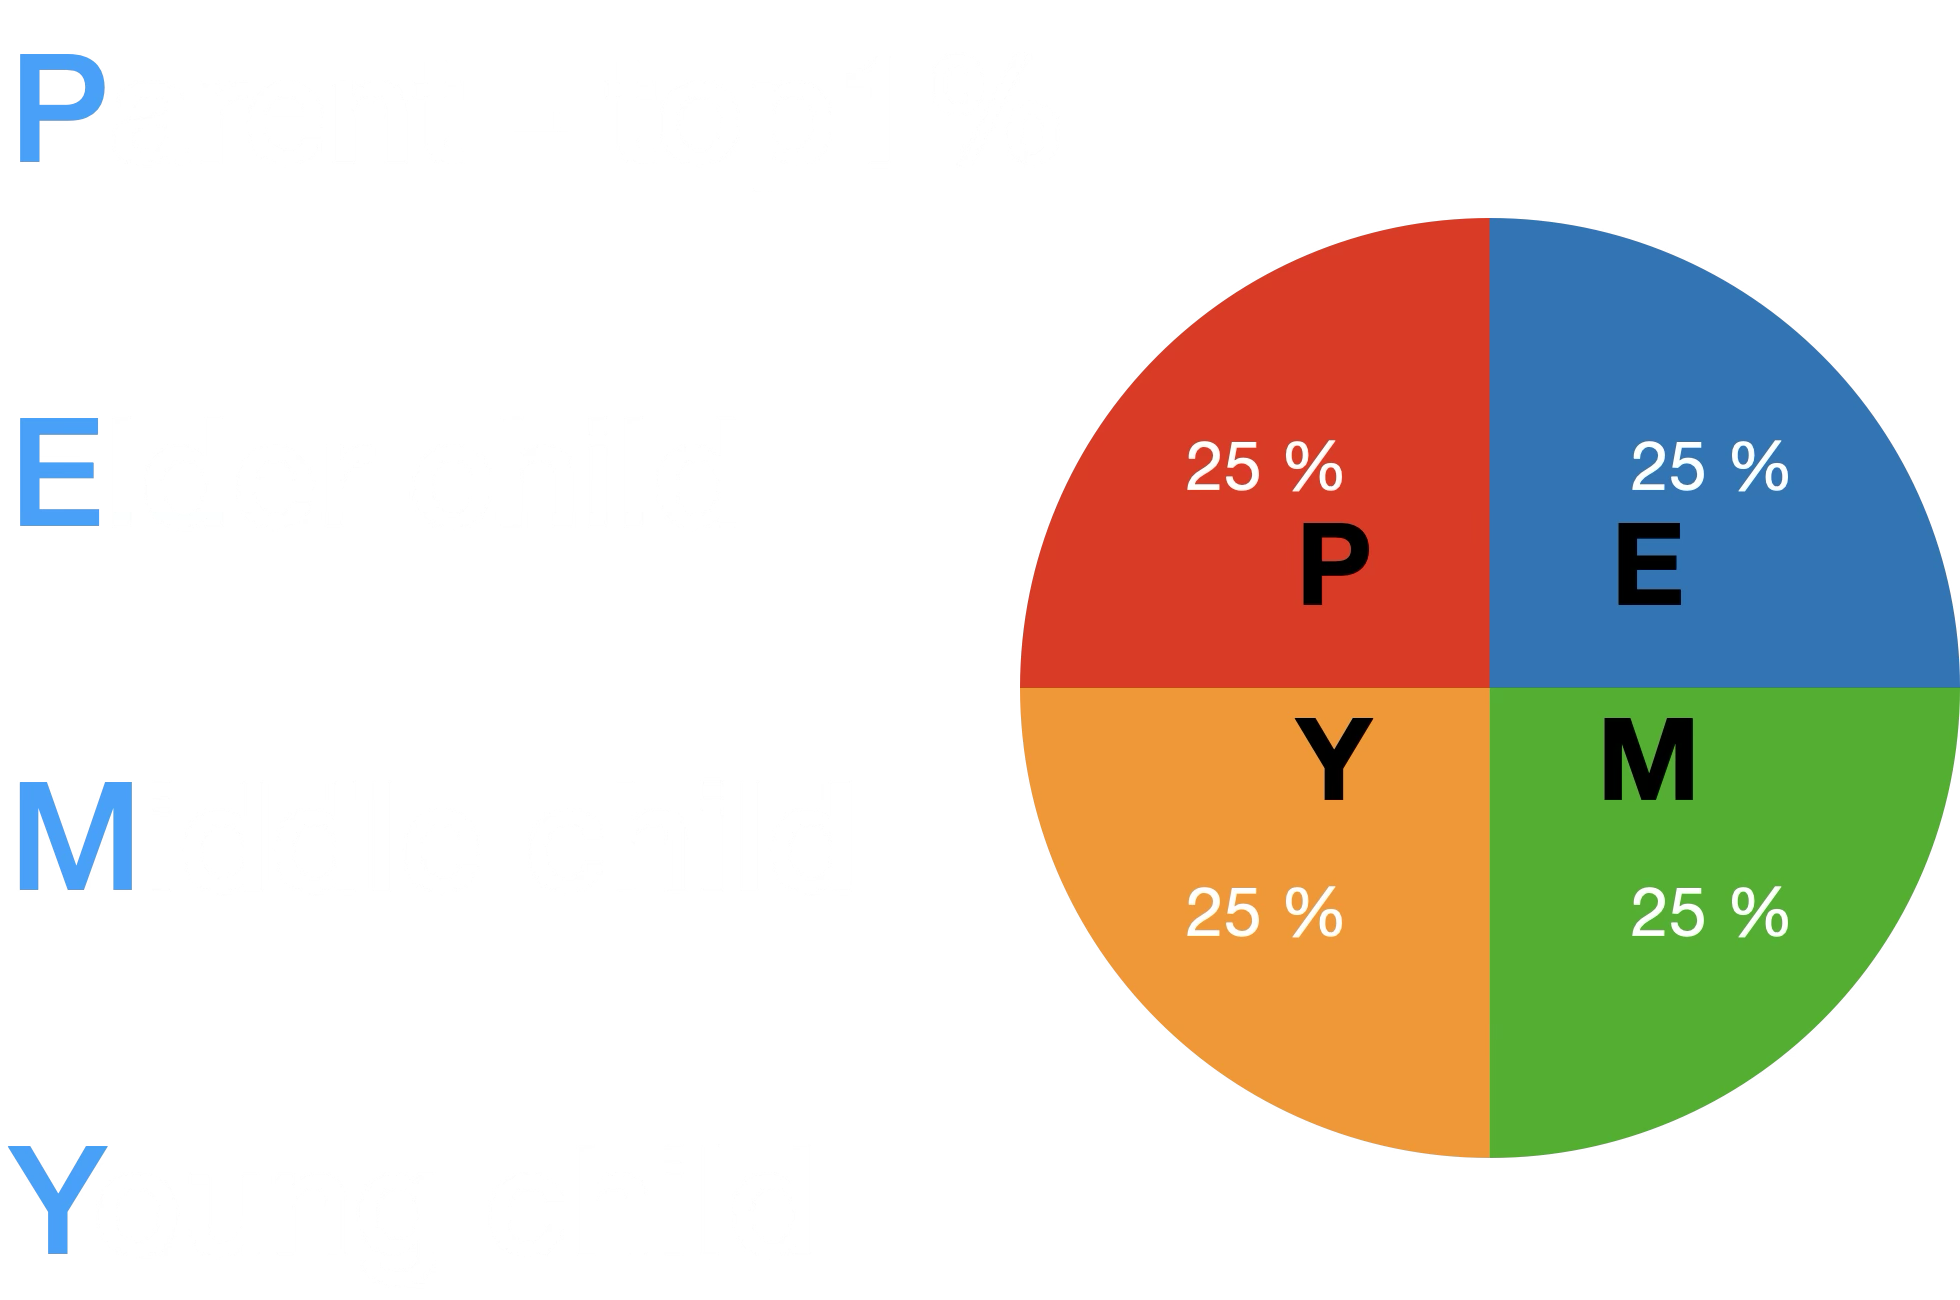
\includegraphics[width=0.8\textwidth]{fig/pemy_part_1.png}
    \caption{\textbf{PEMY Business Model --- Part 1}: Illustration comparing traditional hierarchical ownership (pyramid) with PEMY distributed ownership (circle). In traditional models, value flows upward to shareholders. In PEMY, value circulates among all stakeholders.}
    \label{fig:pemy1}
\end{figure}

\begin{figure}[H]
    \centering
    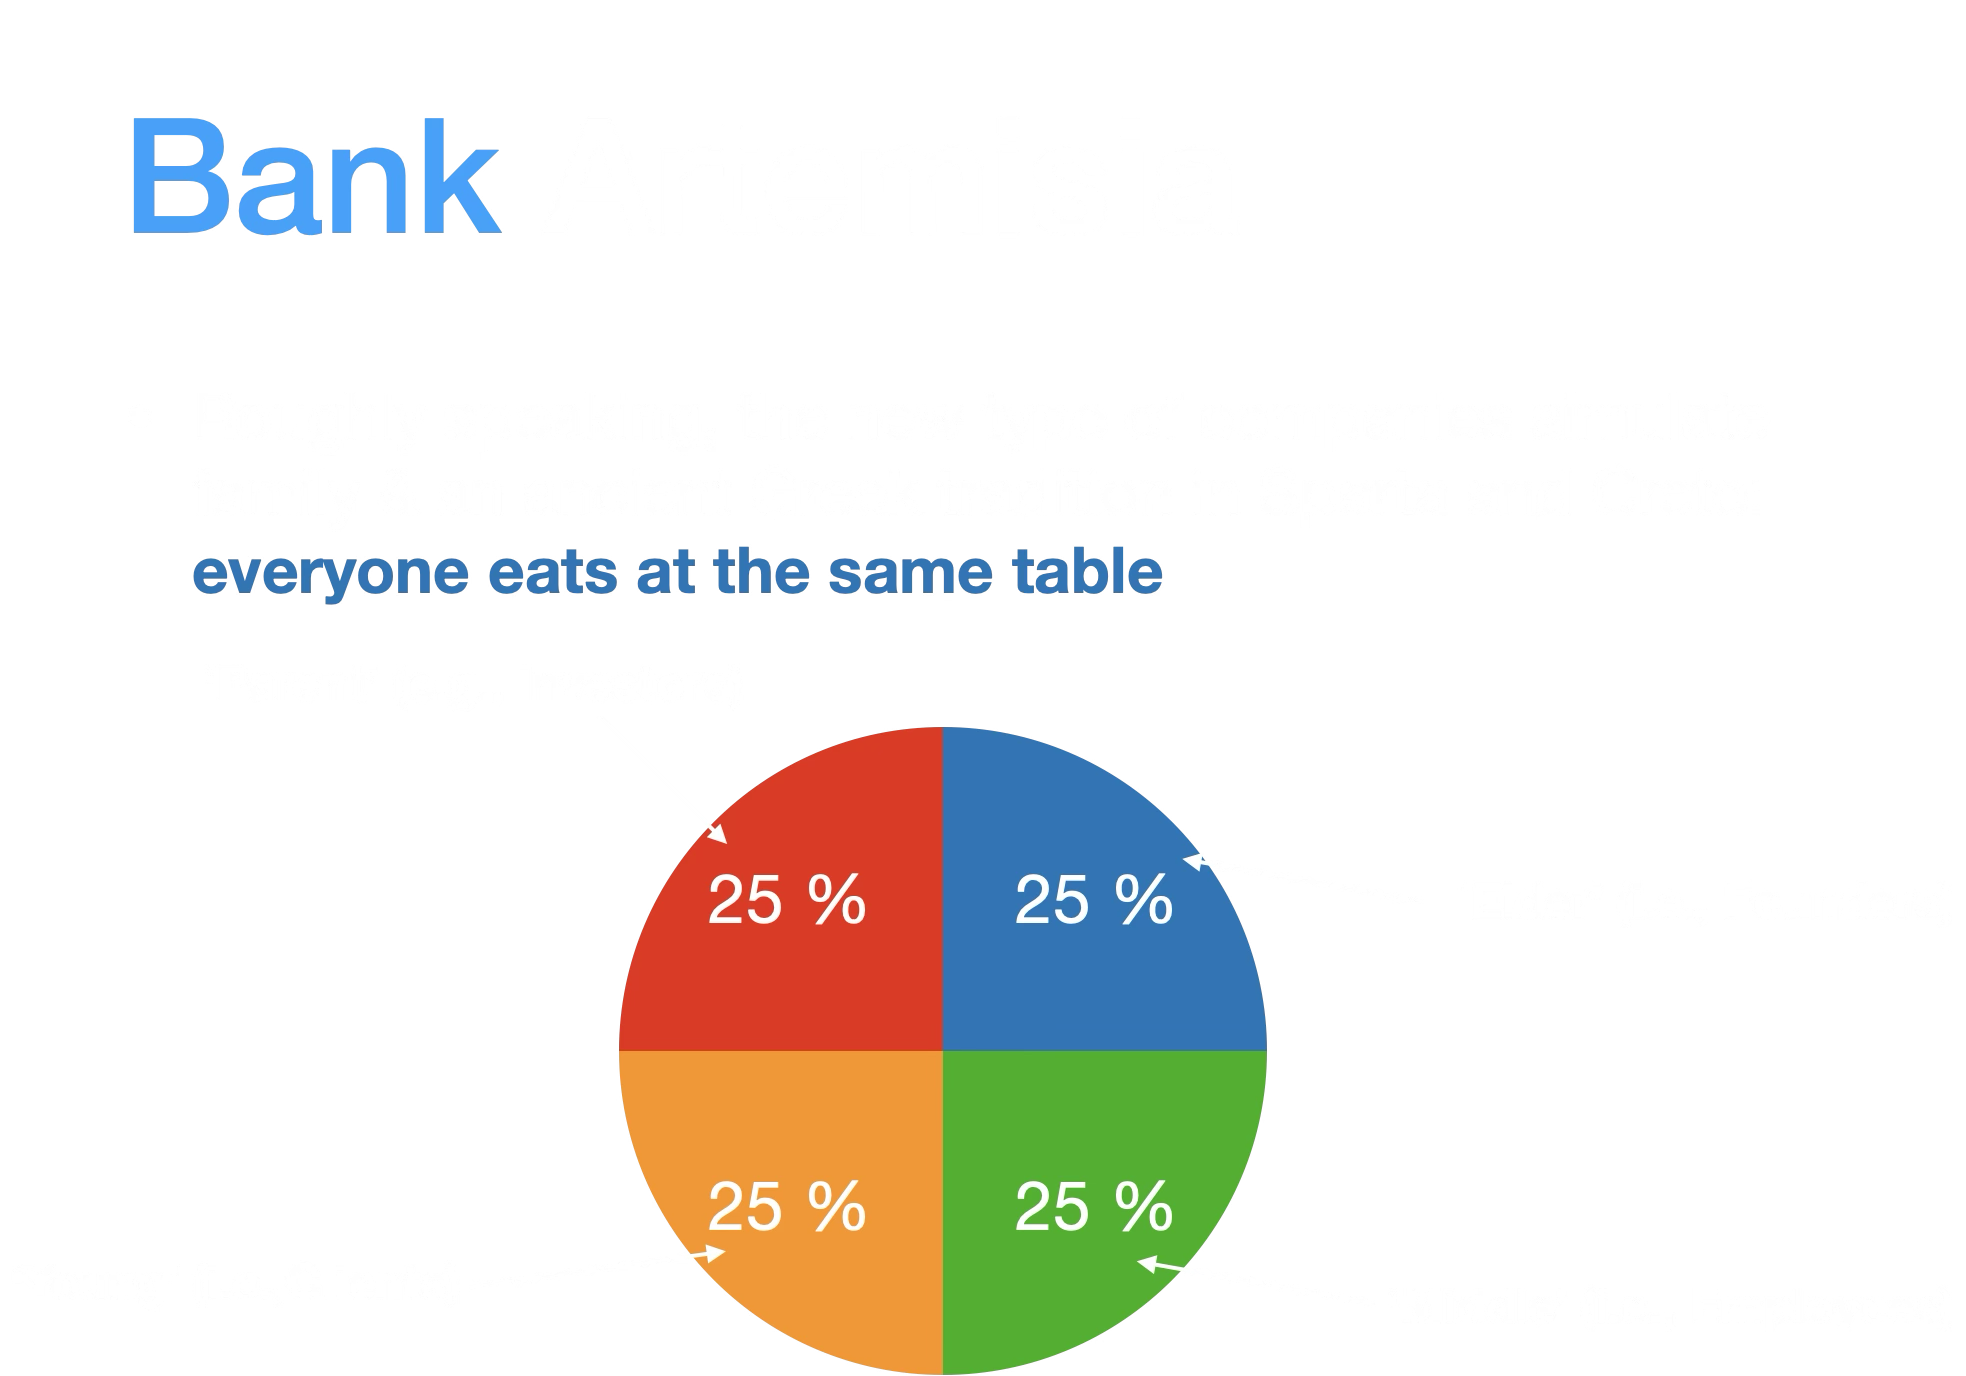
\includegraphics[width=0.8\textwidth]{fig/pemy_part_2.png}
    \caption{\textbf{PEMY Business Model --- Part 2}: Detailed breakdown of ownership percentages and governance structure. Shows how different stakeholder groups (Parent, Elder, Middle, Young) participate in decision-making and benefit-sharing.}
    \label{fig:pemy2}
\end{figure}

\textbf{How PEMY Modifies \SES{} Parameters:}
\begin{itemize}
    \item \textbf{П$_1$ (Values):} Balances profit with wellbeing, sustainability, fairness
    \item \textbf{П$_2$ (Distribution):} Spreads wealth across stakeholders, not concentrated at top
    \item \textbf{П$_3$ (Information):} Mandates transparency, reducing asymmetry
    \item \textbf{П$_4$ (Roles):} Flatter hierarchy, shared ownership identity
    \item \textbf{П$_5$ (Memory):} Builds narrative of cooperation, not extraction
\end{itemize}

\textbf{Advantages Over Traditional Capitalism:}
\begin{itemize}
    \item \textbf{Alignment:} Individual and collective interests converge
    \item \textbf{Resilience:} Diversified ownership provides stability
    \item \textbf{Motivation:} People work for themselves, not for distant shareholders
    \item \textbf{Innovation:} Long-term thinking enables sustainable R\&D
    \item \textbf{Social Cohesion:} Reduces inequality, builds community
\end{itemize}

\textbf{Objections and Responses:}
\begin{itemize}
    \item \textit{``Less profitable'':} Evidence from cooperatives (Mondragon, John Lewis) shows comparable or better performance. Plus, profit for whom? If workers share profits, total wellbeing increases.
    \item \textit{``Requires altruism'':} No---it aligns self-interest with collective interest. Enlightened self-interest, not sacrifice.
    \item \textit{``Just socialism'':} No---retains private ownership, markets, competition. It's capitalism with corrected incentives.
    \item \textit{``How to transition?'':} Gradual, parallel development. PEMY entities compete alongside traditional ones. Market selection over time.
\end{itemize}

\subsection{S.V.E. Cognitive Operating System (S.V.E. X)}

The Cognitive OS \cite{sve10} is a framework for individual and collective awareness, structured around three modes:

\begin{enumerate}
    \item \textbf{Sokrates Mode:} Critical thinking, questioning assumptions
    \begin{itemize}
        \item Tools: Socratic dialogue, falsification, steel-manning
        \item Counters: Dogma, groupthink, confirmation bias
    \end{itemize}
    
    \item \textbf{Solomon Mode:} Wise judgment, integrating multiple perspectives
    \begin{itemize}
        \item Tools: Systems thinking, paradox holding, synthesis
        \item Counters: Black-and-white thinking, reductionism
    \end{itemize}
    
    \item \textbf{Ivan Mode:} Compassionate action, embodied ethics
    \begin{itemize}
        \item Tools: Empathy, service, Christ-Vector alignment
        \item Counters: Apathy, cruelty, dehumanization
    \end{itemize}
\end{enumerate}

\textbf{Application to THE \SYSTEM{} Awareness:}
\begin{itemize}
    \item \textbf{Sokrates:} ``Is this narrative true? Who benefits from it?''
    \item \textbf{Solomon:} ``How do psychological, economic, and spiritual factors interact?''
    \item \textbf{Ivan:} ``What action reduces suffering and increases love?''
\end{itemize}

Regular practice of these modes builds resistance to THE \SYSTEM{}'s unconscious pull.

\subsection{Verifiable Knowledge Base (S.V.E. XI)}

The VKB \cite{sve11} is a decentralized, citation-based system for storing and verifying knowledge:

\textbf{Features:}
\begin{itemize}
    \item \textbf{Source Transparency:} Every claim linked to primary sources
    \item \textbf{Confidence Tracking:} Explicit uncertainty quantification
    \item \textbf{Community Verification:} Crowdsourced fact-checking
    \item \textbf{Version Control:} Track evolution of understanding
    \item \textbf{Dispute Resolution:} Epistemological Boxing for contested claims
\end{itemize}

\textbf{Counters THE \SYSTEM{}'s Information Control (П$_3$):}
\begin{itemize}
    \item Reduces reliance on centralized media
    \item Surfaces hidden assumptions and narratives
    \item Enables collective sensemaking
    \item Builds shared reality foundation
\end{itemize}

\subsection{Self-Information-Purification (SIP) and Epistemological Boxing (EBP)}

S.V.E.~0 \cite{sve0} introduces two complementary protocols:

\textbf{SIP (Self-Information-Purification):}
\begin{enumerate}
    \item Identify a belief you hold
    \item Trace its origins (where did you get it?)
    \item Examine the evidence (is it solid?)
    \item Consider alternatives (what if the opposite were true?)
    \item Hold lightly (be willing to update)
\end{enumerate}

\textbf{EBP (Epistemological Boxing):}
\begin{enumerate}
    \item Define the thesis clearly
    \item Each side presents the \textit{strongest} version of their argument (steel-manning)
    \item Identify cruxes (what evidence would change your mind?)
    \item Test empirically where possible
    \item Update beliefs based on evidence
\end{enumerate}

These protocols counter THE \SYSTEM{}'s tendency to entrench dogma and polarization.

\subsection{Christ-Vector: The Ethical Geodesic}

S.V.E.~IV \cite{sve4} formalizes the Christ-Vector as the geodesic in ethical space---the path that maximizes love and minimizes unnecessary suffering, regardless of religious belief.

\begin{definition}[Christ-Vector]
The Christ-Vector $\vec{C}$ is defined as the solution to:
\[
\vec{C} = \arg\max_{\vec{v}} \left[ \Love(\vec{v}) - \lambda \SScri(\vec{v}) \right]
\]
subject to the constraint of truth alignment: $\vec{v} \cdot \vec{T} > 0$ where $\vec{T}$ is the truth vector.
\end{definition}

\textbf{Practical Translation:}
\begin{itemize}
    \item Act with love (compassion, empathy, service)
    \item Minimize harm (non-violence, care)
    \item Align with truth (honesty, integrity)
    \item Forgive (release resentment, break cycles)
    \item Serve (prioritize others' wellbeing)
\end{itemize}

\textbf{Why ``Christ''-Vector?}
\begin{enumerate}
    \item Historical precedent: Jesus of Nazareth embodied this path
    \item Universal applicability: These principles appear across wisdom traditions
    \item Falsifiable: We can test whether love-oriented actions lead to better outcomes (see Section~\ref{sec:empirical_tests})
    \item Non-sectarian: Accessible to believers and non-believers alike
\end{enumerate}

The Christ-Vector is the antidote to THE \SYSTEM{}'s dehumanizing defaults. It is the ``straight and narrow path'' through the curved post-Fall manifold.

\newpage

% ==================== PART V ====================
\section{Part V: Verification, Falsification, and the Path Forward}

\subsection{Empirical Tests of the THE \SYSTEM{} Framework}
\label{sec:empirical_tests}

The THE \SYSTEM{} hypothesis must be testable. We propose several empirical approaches:

\textbf{Test 1: PEMY vs. Traditional Firms}
\begin{itemize}
    \item \textbf{Hypothesis:} PEMY-structured companies will show higher employee satisfaction, lower turnover, comparable or better financial performance, and greater community benefit
    \item \textbf{Method:} Longitudinal comparison of matched firms (controlling for industry, size, age)
    \item \textbf{Metrics:} Employee wellbeing surveys, retention rates, profit margins, community impact scores
    \item \textbf{Timeline:} 5--10 years
\end{itemize}

\textbf{Test 2: Cognitive OS Training Impact}
\begin{itemize}
    \item \textbf{Hypothesis:} Individuals trained in S.V.E.~X protocols will demonstrate increased awareness of THE \SYSTEM{} dynamics, better critical thinking, reduced susceptibility to manipulation
    \item \textbf{Method:} Randomized controlled trial with pre/post assessments
    \item \textbf{Metrics:} Media literacy scores, bias recognition tests, decision quality, life satisfaction
    \item \textbf{Timeline:} 1--2 years
\end{itemize}

\textbf{Test 3: Community-Level Interventions}
\begin{itemize}
    \item \textbf{Hypothesis:} Communities implementing multiple S.V.E. protocols (VKB, PEMY businesses, Cognitive OS training) will show reduced inequality, increased social cohesion, improved wellbeing
    \item \textbf{Method:} Quasi-experimental design with matched control communities
    \item \textbf{Metrics:} Gini coefficient, trust surveys, health outcomes, crime rates, environmental indicators
    \item \textbf{Timeline:} 10--20 years
\end{itemize}

\textbf{Test 4: Comparative Ethics Outcomes}
\begin{itemize}
    \item \textbf{Hypothesis:} Christ-Vector ethics (love, forgiveness, service) produce better long-term outcomes than alternative frameworks
    \item \textbf{Method:} Identify communities explicitly following different ethical frameworks (Christ-Vector, pure utilitarian, Nietzschean, materialist). Control for size, resources, environment. Measure wellbeing, social cohesion, sustainability, violence, trust over generations.
    \item \textbf{Prediction:} Christ-Vector communities will show highest wellbeing, greatest social cohesion, most sustainable practices, lowest violence, highest trust
\end{itemize}

\begin{remark}[Independence from Belief]
Test 4 is designed to reveal objective truth (Logos) independent of religious belief. If the predictions hold, it suggests Christ-Vector represents alignment with reality structure, not merely cultural preference. This would be profound evidence for geodesic ethics as described in \cite{sve4,sve8}.
\end{remark}

\subsection{Broader Implications}

If the THE \SYSTEM{} framework is validated, implications span multiple domains:

\textbf{Political:}
\begin{itemize}
    \item Current governance structures may be fundamentally captured by THE \SYSTEM{}
    \item True democracy requires collective awareness (Cognitive OS for citizenry)
    \item Transparency and verification (à la Fakten-TÜV from S.V.E.~X) essential
    \item National boundaries may need rethinking for global cooperation
\end{itemize}

\textbf{Economic:}
\begin{itemize}
    \item GDP as metric is THE \SYSTEM{}-aligned (growth über alles)
    \item Alternative metrics needed (wellbeing, sustainability, equality)
    \item Financial systems may require redesign (re-linking money to real value)
    \item PEMY or similar models could transform capitalism incrementally
\end{itemize}

\textbf{Educational:}
\begin{itemize}
    \item Current education systems serve THE \SYSTEM{} more than students (Russell's critique)
    \item Critical thinking, meditation, systemic analysis should be core curriculum
    \item Generalists and synthesizers need cultivation, not just specialists
    \item Philosophy and ethics should be central, not peripheral
\end{itemize}

\begin{table}[h]
\centering
\caption{Dual Function of Education within the SYSTEM}
\label{tab:education_duality}
\begin{tabular}{|l|l|}
\hline
\textbf{Enlightening Function} & \textbf{Indoctrinating Function} \\ \hline
Promotes critical thinking and individuation & Reinforces conformity and obedience \\ \hline
Encourages creativity and questioning & Standardizes perception and behavior \\ \hline
Facilitates self-awareness & Suppresses dissenting cognition \\ \hline
\end{tabular}
\end{table}


\textbf{Cultural:}
\begin{itemize}
    \item Mindfulness commodification is symptom, not solution
    \item True awareness requires systemic change, not just individual practice
    \item Media literacy essential in attention economy
    \item Gender norms, sexuality, identity may need de-politicization and re-humanization
\end{itemize}

\begin{figure}[h]
\centering
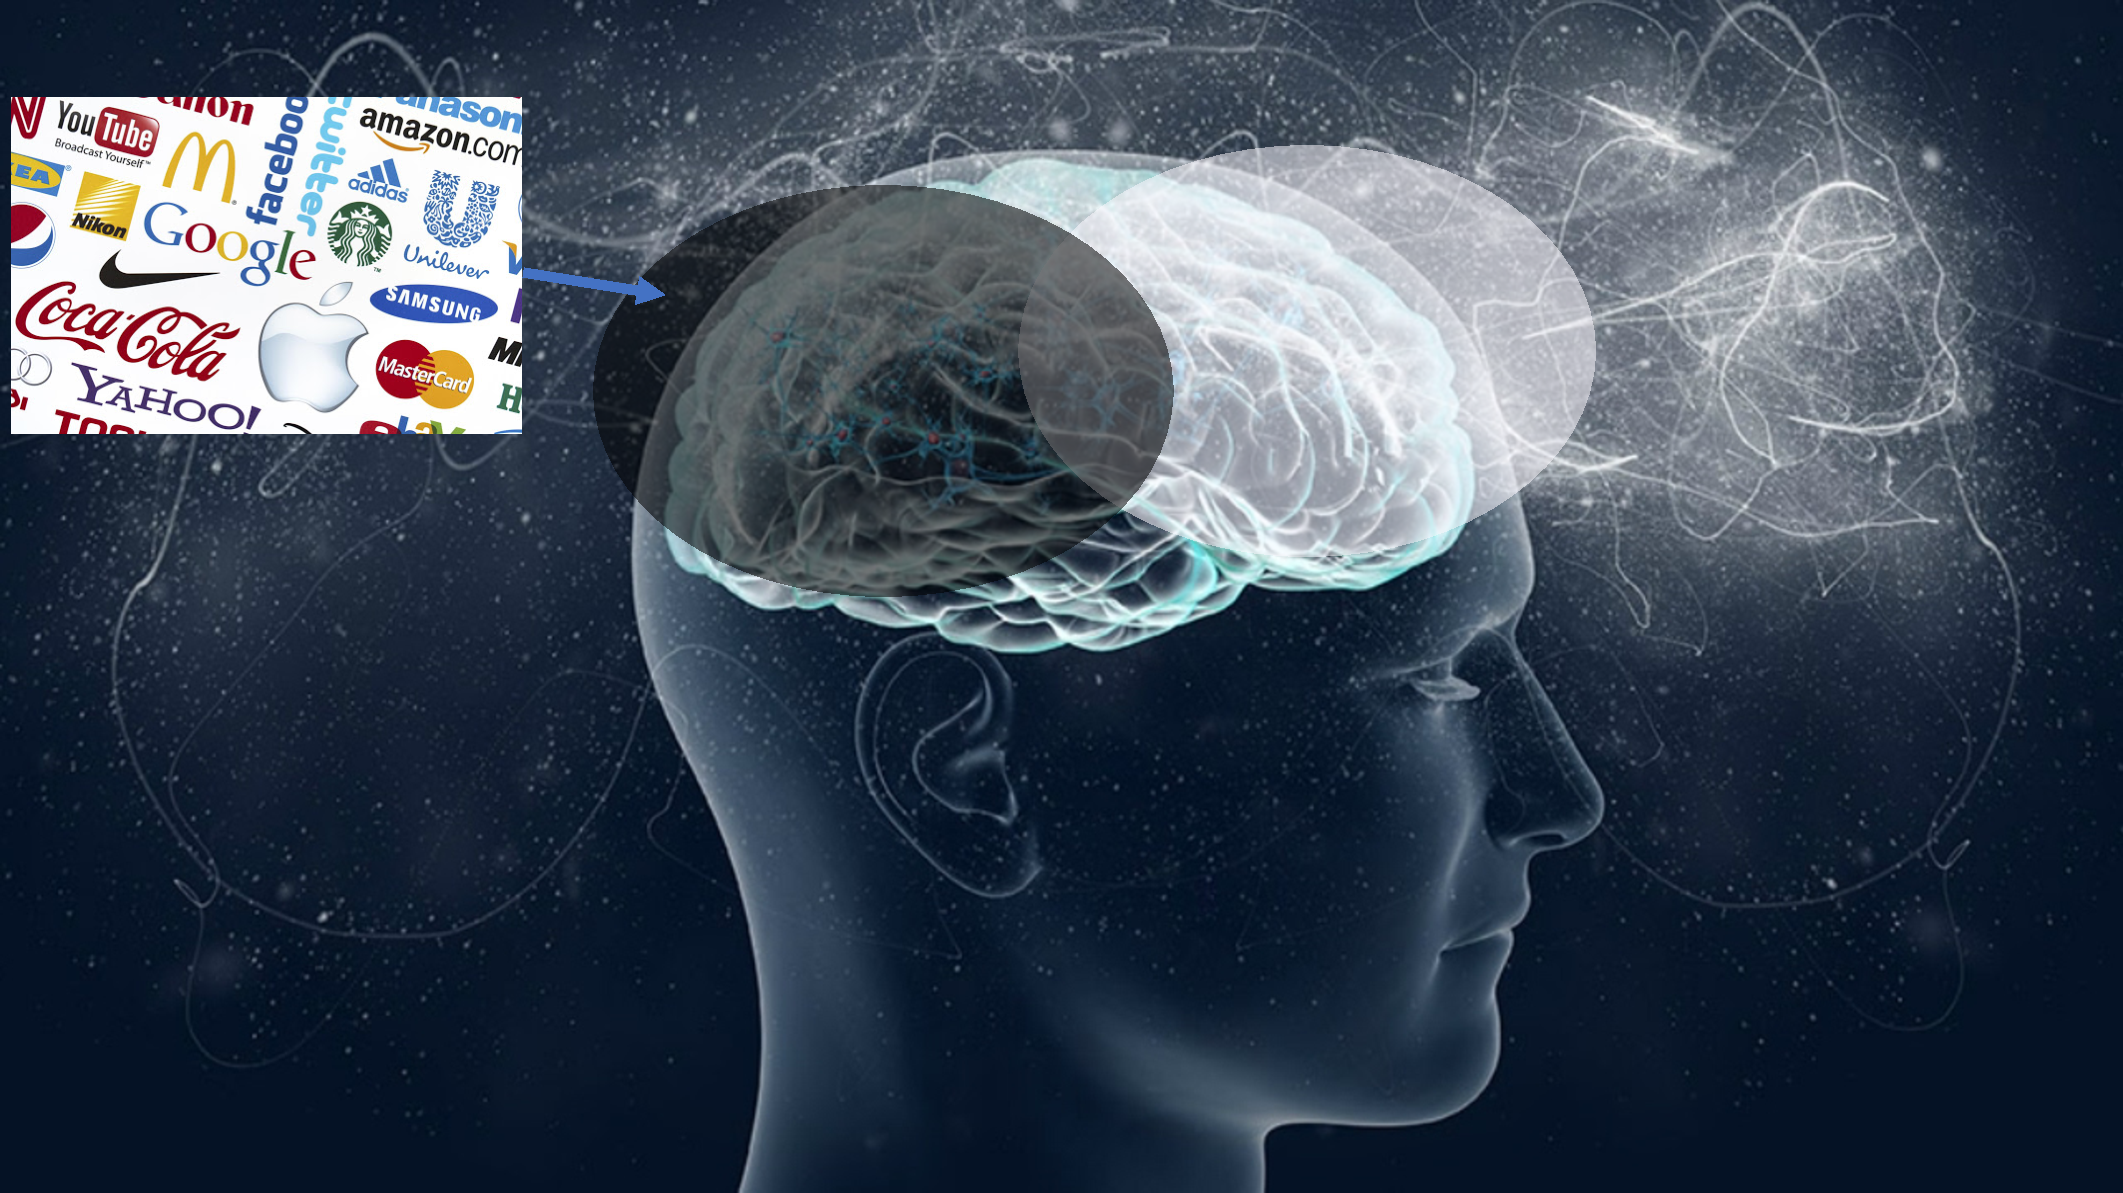
\includegraphics[width=0.9\linewidth]{fig/attention_economy_brands_as_real_estates_in_conciousness_space.pdf}
\caption{Brands as real estate in the cognitive landscape — visualization of attention economy colonization.}
\label{fig:attention_economy}
\end{figure}


\textbf{Spiritual:}
\begin{itemize}
    \item Traditional wisdom (Bible, Buddha, Lao Tzu, etc.) may encode THE \SYSTEM{}-resistant knowledge
    \item Spiritual practices valuable as tools for awareness, not escapism
    \item ``Kingdom within'' redirects from external dopamine loops
    \item Collective healing requires addressing collective trauma
\end{itemize}

\textbf{Technological:}
\begin{itemize}
    \item AI risk discourse should include THE \SYSTEM{} capture scenarios
    \item Surveillance tech accelerates path toward Matrix endpoint
    \item Digitization can assist or exploit depending on ownership structure
    \item Open-source and decentralized systems more resistant to capture
\end{itemize}

\begin{figure}[h]
\centering
\includegraphics[width=0.75\linewidth]{fig/where_humanity_goes.png}
\caption{“Where humanity goes?” — an allegorical reflection on collective uncertainty.}
\label{fig:humanity_future}
\end{figure}


\subsection{The Path Forward}

% Философские корни (старт Part I / Plato)
\begin{figure}[h]\centering
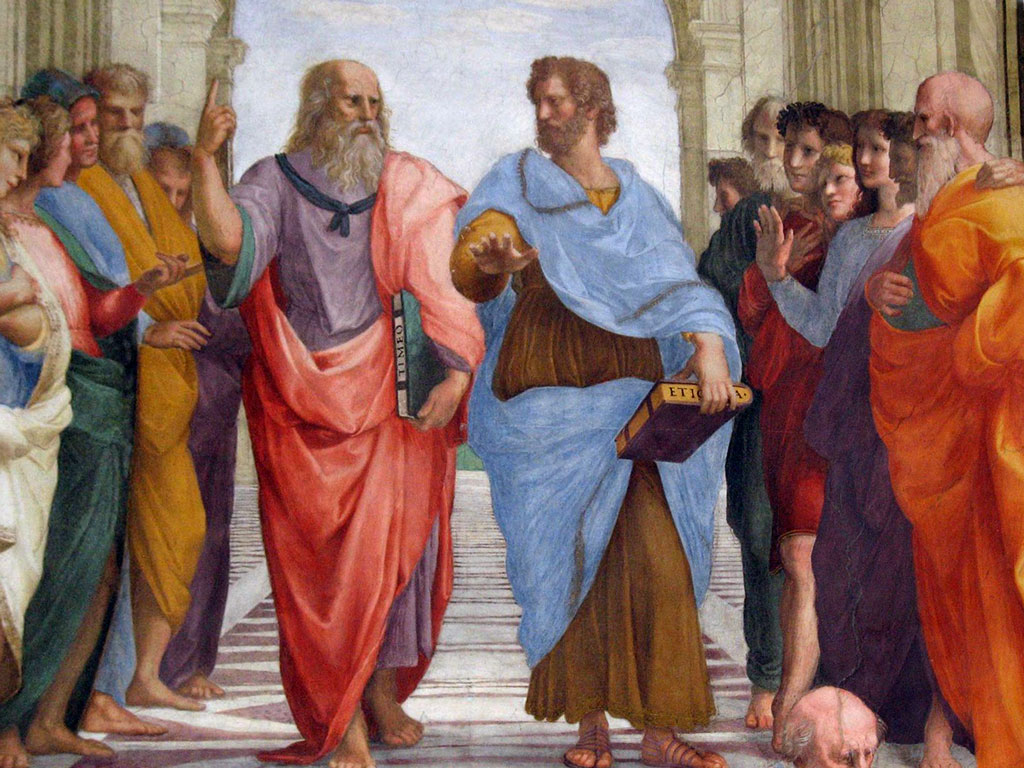
\includegraphics[width=0.7\linewidth]{fig/plato_socrates.jpeg}
\caption{Philosophical roots (Plato/Aristotle) for dialogue with the Cave allegory.}
\label{fig:plato_roots}
\end{figure}


This paper is not a conclusion but an opening. The framework is offered for:

\begin{enumerate}
    \item \textbf{Rigorous critique:} Epistemological Boxing (S.V.E.~0) welcomes adversarial testing
    \item \textbf{Empirical validation:} Tests proposed above should be implemented
    \item \textbf{Collaborative refinement:} Community input via Verifiable Knowledge Base
    \item \textbf{Practical implementation:} PEMY pilots, Cognitive OS training, policy advocacy
    \item \textbf{Cultural dissemination:} Ideas need to propagate as counter-waves to THE \SYSTEM{} patterns
\end{enumerate}

\begin{mdframed}[backgroundcolor=yellow!10]
\textbf{Final Reflection:}

The THE \SYSTEM{} is not evil---it is unconscious. It operates according to logic formed during humanity's traumatic history. Our task is not to destroy it but to \textit{bring it into consciousness}, integrate the split, heal the trauma, and align collective dynamics with long-term flourishing.

This is the most challenging work imaginable: transforming the collective unconscious itself. But it is also the most necessary. The alternative---continuing on the current trajectory toward the Matrix endpoint---is unacceptable.

We cannot solve our problems with the same thinking that created them. We need new frameworks, new practices, new structures. The S.V.E. series offers one such framework. May it serve as a catalyst for the collective awakening we so desperately need.

\begin{figure}[h]
\centering
\includegraphics[width=0.75\linewidth]{fig/zmeya_poedaet_sebya_illustration_of_dynamics.png}
\caption{The SYSTEM as an Ouroboros — a self-consuming feedback loop symbolizing cyclical self-destruction.}
\label{fig:ouroboros}
\end{figure}


\textit{``By their fruits you shall know them.''} Let us test these ideas rigorously, implement them courageously, and judge them by their outcomes. The future depends on our willingness to see clearly, think deeply, and act wisely---together.
\end{mdframed}

\subsection{A Challenge to the Reader}

We close with a direct challenge:

\textbf{If you disagree with this framework:}
\begin{itemize}
    \item Identify specific axioms, propositions, or claims that are false
    \item Propose alternative explanations for the phenomena described
    \item Engage in Epistemological Boxing to test our respective models
\end{itemize}

\textbf{If you agree with this framework:}
\begin{itemize}
    \item Identify weaknesses, gaps, or areas needing refinement
    \item Propose additional empirical tests
    \item Implement S.V.E. protocols in your own life and communities
    \item Contribute to the Verifiable Knowledge Base
\end{itemize}

\textbf{If you are uncertain:}
\begin{itemize}
    \item Hold the framework as a hypothesis, not a conclusion
    \item Observe your own life and society through this lens
    \item Test small predictions (e.g., ``If I practice Cognitive OS, will my decision quality improve?'')
    \item Engage in dialogue with others exploring these ideas
\end{itemize}

The THE \SYSTEM{} thrives in unconsciousness. Every act of awareness, every moment of critical thinking, every choice aligned with love over fear---these are acts of resistance and healing.

\noindent
For actionable governance aligned with the analysis above, see the PEMY framework in Appendix~\ref{app:pemy_principles}--\ref{app:pemy_cases}, which operationalizes interventions across P1--P5 with reversibility and open audits.


\vspace{1em}

\begin{center}
\textbf{С Богом! --- With God!} (For those who believe) \\
\textbf{С Любовью! --- With Love!} (For all)
\end{center}

\vspace{1em}

\textit{May this work serve Truth and contribute to the healing of our shared consciousness.}

\newpage

\section*{AI Commentary (Independent Review Notes)}
Summaries of interpretive and analytical feedback were produced by independent AI systems 
(\textit{e.g.}, OpenAI GPT-5, Anthropic Claude, Google Gemini) 
for the purposes of metacognitive audit and narrative clarity verification.  

For full AI-based interpretive reviews, see the supplementary repository:  
\href{https://github.com/skovnats/SVE-Systemic-Verification-Engineering/tree/master/Reviews}{github.com/skovnats/Reviews}


% ==================== BIBLIOGRAPHY ====================
\bibliographystyle{plainnat}
\bibliography{ref.bib}

\newpage

% ==================== APPENDICES ====================
% ==================== COMPLETE INTEGRATED APPENDIX ====================
% This complete appendix replaces everything after the main body in arXiv.tex
% Insert before \end{document}

\appendix

% ==================== MATHEMATICAL FOUNDATIONS ====================
\section{Mathematical Foundations and Extended Proofs}
\label{app:math_foundations}

This appendix provides rigorous mathematical formulations, proofs, and extended derivations for the core theoretical constructs of S.V.E. XII. We formalize the \SESES\ manifold structure, derive the $\delta$-dehumanization dynamics, and establish the geodesic optimization framework.

\subsection{The SESES Manifold: Formal Construction}
\label{app:seses_manifold}

\begin{definition}[SESES Manifold]
Let $\mathcal{M}_{\SESES}$ be an $n$-dimensional smooth differentiable manifold with $n \geq 8$, representing the state space of a civilization's socio-economic-spiritual-emotional configuration. Each point $X(t) \in \mathcal{M}_{\SESES}$ is characterized by:
\[
X(t) = \bigl(E(t), S(t), P(t), C(t), M(t), I(t), G(t), Em(t)\bigr)
\]
where:
\begin{itemize}[leftmargin=1.5em]
    \item $E(t)$: Economic state (production, distribution, wealth)
    \item $S(t)$: Social structure (power distribution, trust networks)
    \item $P(t)$: Political configuration (governance, decision rights)
    \item $C(t)$: Cultural state (values, narratives, meaning systems)
    \item $M(t)$: Material-ecological state (resources, environment)
    \item $I(t)$: Information-epistemic state (knowledge quality, truth access)
    \item $G(t)$: Governance-institutional state (rule systems, enforcement)
    \item $Em(t)$: Emotional-spiritual state (collective wellbeing, consciousness)
\end{itemize}
\end{definition}

\begin{definition}[SESES Metric Tensor]
The manifold $\mathcal{M}_{\SESES}$ is endowed with a pseudo-Riemannian metric tensor $g_{\mu\nu}(X)$ that encodes the ``ethical distance'' or transformation cost between states. The line element is:
\[
ds^2 = g_{\mu\nu}(X) \, dX^\mu \, dX^\nu
\]
The metric components represent:
\begin{itemize}[leftmargin=1.5em]
    \item Diagonal terms $g_{\mu\mu}$: inertia or resistance to change within dimension $\mu$
    \item Off-diagonal terms $g_{\mu\nu}$ ($\mu \neq \nu$): coupling between dimensions---how change in dimension $\mu$ affects dimension $\nu$
\end{itemize}
\end{definition}

\begin{proposition}[Christoffel Symbols and Socio-Economic Coupling]
The Christoffel symbols of the second kind,
\[
\Gamma^\lambda_{\mu\nu} = \frac{1}{2} g^{\lambda\sigma} \left( \partial_\mu g_{\sigma\nu} + \partial_\nu g_{\mu\sigma} - \partial_\sigma g_{\mu\nu} \right),
\]
encode the interdependence structure of socio-economic dimensions. Specifically:
\begin{enumerate}[leftmargin=1.5em]
    \item Large $\Gamma^E_{SP}$ indicates economic state $E$ is strongly affected by changes in social $S$ and political $P$ dimensions
    \item Asymmetric patterns $\Gamma^\mu_{\nu\lambda} \neq \Gamma^\mu_{\lambda\nu}$ would indicate path-dependent transformation costs
    \item The trace $\Gamma^\mu_{\mu\nu}$ measures systemic coupling strength along dimension $\nu$
\end{enumerate}
\end{proposition}

\begin{theorem}[Curvature as Systemic Rigidity]
The Riemann curvature tensor
\[
R^\rho{}_{\sigma\mu\nu} = \partial_\mu \Gamma^\rho_{\nu\sigma} - \partial_\nu \Gamma^\rho_{\mu\sigma} + \Gamma^\rho_{\mu\lambda} \Gamma^\lambda_{\nu\sigma} - \Gamma^\rho_{\nu\lambda} \Gamma^\lambda_{\mu\sigma}
\]
quantifies the obstruction to parallel transport of societal state vectors. Non-zero curvature indicates:
\begin{enumerate}[leftmargin=1.5em]
    \item \textbf{Systemic trauma:} regions where past events create path-dependent constraints
    \item \textbf{Structural rigidity:} inability to return to initial states after closed loops in policy space
    \item \textbf{Institutional memory:} embedding of historical patterns in the manifold geometry
\end{enumerate}
The scalar curvature $R = g^{\mu\nu} R_{\mu\nu}$ provides a single-number measure of overall systemic rigidity.
\end{theorem}

\begin{proof}
Consider a vector field $V^\mu$ representing a policy direction. Under parallel transport around a closed loop in the $(\mu,\nu)$ plane, the change in $V^\rho$ is:
\[
\Delta V^\rho = \oint R^\rho{}_{\sigma\mu\nu} V^\sigma \, dA^{\mu\nu}
\]
where $dA^{\mu\nu}$ is the area element. If $R^\rho{}_{\sigma\mu\nu} = 0$, policies return to their initial orientation---the system has no memory of the loop. Non-zero curvature means the system ``remembers'' the traversal through accumulated structural change, representing irreversible institutional transformation.
\end{proof}

\subsection{Socio-Economic Field Theory}
\label{app:field_theory}

\begin{definition}[Value-Flow Potential]
Define a vector potential $A_\mu(X)$ on $\mathcal{M}_{\SESES}$ where:
\begin{itemize}[leftmargin=1.5em]
    \item $A_E$: economic value flow potential (capital circulation)
    \item $A_I$: information flow potential (knowledge distribution)
    \item $A_{Em}$: emotional-spiritual energy potential (collective consciousness)
\end{itemize}
The potential satisfies the gauge freedom $A_\mu \to A_\mu + \partial_\mu \chi$ for any scalar function $\chi$, representing freedom in choosing value measurement scales.
\end{definition}

\begin{definition}[Socio-Economic Field Tensor]
The field strength tensor is defined as:
\[
F_{\mu\nu} = \nabla_\mu A_\nu - \nabla_\nu A_\mu = \partial_\mu A_\nu - \partial_\nu A_\mu
\]
(In flat coordinates, the covariant derivative reduces to partial derivative). This tensor is antisymmetric and gauge-invariant, representing observable flow imbalances.
\end{definition}

\begin{proposition}[Stress-Energy Tensor]
Define the stress-energy tensor for the socio-economic field:
\[
T_{\mu\nu} = F_{\mu\lambda} F_\nu{}^\lambda - \frac{1}{4} g_{\mu\nu} F_{\alpha\beta} F^{\alpha\beta}
\]
This tensor has the following interpretation:
\begin{itemize}[leftmargin=1.5em]
    \item $T_{00}$: total systemic energy density (productive + destructive)
    \item $T_{0i}$: momentum flow (value transfer rates)
    \item $T_{ij}$: stress components (tension between dimensions)
\end{itemize}
\end{proposition}

\begin{theorem}[Conservation Law]
The stress-energy tensor satisfies the conservation equation:
\[
\nabla^\mu T_{\mu\nu} = 0
\]
expressing conservation of total socio-economic-ethical energy-momentum.
\end{theorem}

\begin{proof}
From the definition of $T_{\mu\nu}$ and the antisymmetry of $F_{\mu\nu}$:
\begin{align*}
\nabla^\mu T_{\mu\nu} &= \nabla^\mu \left( F_{\mu\lambda} F_\nu{}^\lambda - \frac{1}{4} g_{\mu\nu} F_{\alpha\beta} F^{\alpha\beta} \right) \\
&= (\nabla^\mu F_{\mu\lambda}) F_\nu{}^\lambda + F_{\mu\lambda} \nabla^\mu F_\nu{}^\lambda - \frac{1}{2} g_{\mu\nu} F^{\alpha\beta} \nabla^\mu F_{\alpha\beta}
\end{align*}
Using the Bianchi identity $\nabla_{[\alpha} F_{\beta\gamma]} = 0$ (which follows from $F_{\mu\nu} = \partial_\mu A_\nu - \partial_\nu A_\mu$), we obtain $\nabla^\mu F_{\mu\lambda} = 0$. The remaining terms cancel by antisymmetry, yielding the conservation law.

\textbf{Physical interpretation:} Ethical-economic value cannot be created or destroyed in isolation---it can only be redistributed or transformed between dimensions of \SESES. Apparent ``value destruction'' (e.g., in financial crises) represents transformation into hidden costs (social $S$, emotional $Em$, ecological $M$ dimensions).
\end{proof}

\subsection{The $\delta$-Dehumanization Dynamic: Rigorous Derivation}
\label{app:delta_dynamics}

\begin{definition}[Dehumanization Index $\delta$]
The dehumanization index at state $X$ is defined as:
\[
\delta(X) = \left\| \Phi(X) \right\|_g^2 = g^{\mu\nu}(X) \, \Phi_\mu(X) \, \Phi_\nu(X)
\]
where $\Phi_\mu(X)$ is the gradient of collective suffering potential:
\[
\Phi_\mu = \frac{\partial \mathcal{S}}{\partial X^\mu}
\]
and $\mathcal{S}(X)$ is the total suffering functional defined as:
\[
\mathcal{S}(X) = \int_{\text{population}} s(X, \text{individual}) \, d(\text{individual})
\]
where $s$ measures individual suffering as a function of societal state.
\end{definition}

\begin{proposition}[Five Pathological Levers]
The dehumanization index can be decomposed into contributions from five primary mechanisms:
\[
\delta(X) = \sum_{i=1}^5 w_i \cdot P_i(X) + \mathcal{O}(\text{interactions})
\]
where:
\begin{align*}
P_1(X) &= \text{information opacity} = -\frac{\partial I}{\partial t} \Big/ \left\| \nabla_t I \right\|_{\text{truth}} \\
P_2(X) &= \text{attention monopoly} = H_{\text{attention}}^{-1} \cdot C_{\text{HH}}^{\text{attention}} \\
P_3(X) &= \text{perverse incentives} = \left\| \nabla E - \nabla \mathcal{W} \right\|_g \\
P_4(X) &= \text{bureaucratic inertia} = \text{tr}(g_{GG}) \cdot \tau_{\text{reform}} \\
P_5(X) &= \text{conditioning} = \left\| C_{\text{imposed}} - C_{\text{authentic}} \right\|_2
\end{align*}
Here $H$ is Shannon entropy, $C_{\text{HH}}$ is the Herfindahl-Hirschman index, $\mathcal{W}$ is wellbeing, $\tau$ is reform timescale, and norms measure divergence in respective spaces.
\end{proposition}

\begin{theorem}[Delta Flow Equation]
The time evolution of $\delta$ along a trajectory $X(t)$ in \SESES\ space is governed by:
\[
\frac{d\delta}{dt} = 2 g^{\mu\nu} \Phi_\mu \, \nabla_t \Phi_\nu + \left( \nabla_t g^{\mu\nu} \right) \Phi_\mu \Phi_\nu
\]
where $\nabla_t = \frac{d}{dt}$ is the covariant time derivative along the trajectory.
\end{theorem}

\begin{proof}
Starting from the definition $\delta = g^{\mu\nu} \Phi_\mu \Phi_\nu$, we compute:
\begin{align*}
\frac{d\delta}{dt} &= \frac{d}{dt}\left( g^{\mu\nu} \Phi_\mu \Phi_\nu \right) \\
&= \left( \frac{dg^{\mu\nu}}{dt} \right) \Phi_\mu \Phi_\nu + g^{\mu\nu} \left( \frac{d\Phi_\mu}{dt} \right) \Phi_\nu + g^{\mu\nu} \Phi_\mu \left( \frac{d\Phi_\nu}{dt} \right) \\
&= \left( \nabla_t g^{\mu\nu} \right) \Phi_\mu \Phi_\nu + g^{\mu\nu} (\nabla_t \Phi_\mu) \Phi_\nu + g^{\mu\nu} \Phi_\mu (\nabla_t \Phi_\nu) \\
&= \left( \nabla_t g^{\mu\nu} \right) \Phi_\mu \Phi_\nu + 2 g^{\mu\nu} \Phi_\mu \, \nabla_t \Phi_\nu
\end{align*}
where we used the symmetry of $g^{\mu\nu}$ and the product rule.
\end{proof}

\begin{corollary}[Conditions for $\delta$-Reduction]
For $\frac{d\delta}{dt} < 0$ (decreasing dehumanization), it is necessary that:
\[
g^{\mu\nu} \Phi_\mu \, \nabla_t \Phi_\nu < -\frac{1}{2} \left( \nabla_t g^{\mu\nu} \right) \Phi_\mu \Phi_\nu
\]
This requires steering the trajectory so that suffering gradients decrease faster than the metric structure changes.
\end{corollary}

\begin{definition}[SYSTEM Attractor Region]
Define $\Omega_{\SYSTEM} \subset \mathcal{M}_{\SESES}$ as the region where:
\[
\Omega_{\SYSTEM} = \left\{ X \in \mathcal{M}_{\SESES} \,:\, \delta(X) > \delta_{\text{crit}} \wedge \frac{d\delta}{dt}\Big|_{\text{natural}} > 0 \right\}
\]
where ``natural'' refers to trajectories under current socio-economic dynamics without conscious intervention. Points in $\Omega_{\SYSTEM}$ exhibit self-amplifying dehumanization.
\end{definition}

\begin{theorem}[Stability of SYSTEM Attractor]
Let $\lambda_1, \ldots, \lambda_n$ be the eigenvalues of the Jacobian $J_\mu{}^\nu = \frac{\partial V^\nu}{\partial X^\mu}$ evaluated at a fixed point $X_* \in \Omega_{\SYSTEM}$, where $V^\mu$ is the velocity field. If all $\text{Re}(\lambda_i) > 0$, then $X_*$ is an unstable node requiring active effort to escape. If $\exists i : \text{Re}(\lambda_i) > 0$ and $\exists j : \text{Re}(\lambda_j) < 0$, then $X_*$ is a saddle point with escape directions along eigenvectors corresponding to negative eigenvalues.
\end{theorem}

\begin{proof}
Standard result from dynamical systems theory. Linear stability analysis near fixed point $X_*$:
\[
\delta X(t) \approx \sum_i c_i e^{\lambda_i t} v_i
\]
where $v_i$ are eigenvectors. Positive real parts indicate exponential growth away from equilibrium in those directions; negative real parts indicate attraction. For escape from \SYSTEM, we must align interventions with eigenvectors having $\text{Re}(\lambda) < 0$.
\end{proof}

\subsection{Geodesic Ethics and the Christ-Vector}
\label{app:geodesic_ethics}

\begin{definition}[Ethical Action Functional]
Define the action functional for a trajectory $\gamma: [t_0, t_1] \to \mathcal{M}_{\SESES}$:
\[
\mathcal{A}[\gamma] = \int_{t_0}^{t_1} \left[ \frac{1}{2} g_{\mu\nu} \frac{dX^\mu}{dt} \frac{dX^\nu}{dt} + \lambda \cdot \mathcal{S}(X(t)) \right] dt
\]
where $\lambda > 0$ is a Lagrange multiplier weighting suffering against transformation cost.
\end{definition}

\begin{theorem}[Euler-Lagrange Equations for Ethical Geodesics]
The trajectory that extremizes $\mathcal{A}$ satisfies:
\[
\frac{d^2 X^\mu}{dt^2} + \Gamma^\mu_{\nu\lambda} \frac{dX^\nu}{dt} \frac{dX^\lambda}{dt} = -\lambda \, g^{\mu\nu} \frac{\partial \mathcal{S}}{\partial X^\nu}
\]
These are the geodesic equations with a forcing term proportional to the suffering gradient.
\end{theorem}

\begin{proof}
The Euler-Lagrange equations for the Lagrangian 
\[
L = \frac{1}{2} g_{\mu\nu} \dot{X}^\mu \dot{X}^\nu + \lambda \mathcal{S}(X)
\]
are:
\[
\frac{d}{dt}\left( \frac{\partial L}{\partial \dot{X}^\mu} \right) - \frac{\partial L}{\partial X^\mu} = 0
\]
Computing:
\[
\frac{\partial L}{\partial \dot{X}^\mu} = g_{\mu\nu} \dot{X}^\nu
\]
\[
\frac{d}{dt}\left( g_{\mu\nu} \dot{X}^\nu \right) = \partial_\lambda g_{\mu\nu} \dot{X}^\lambda \dot{X}^\nu + g_{\mu\nu} \ddot{X}^\nu
\]
\[
\frac{\partial L}{\partial X^\mu} = \frac{1}{2} \partial_\mu g_{\nu\lambda} \dot{X}^\nu \dot{X}^\lambda + \lambda \partial_\mu \mathcal{S}
\]
Substituting and using the definition of Christoffel symbols yields the stated equation.
\end{proof}

\begin{definition}[Christ-Vector]
The \textbf{Christ-vector} $\vec{\xi}(X)$ at point $X$ is defined as the tangent direction to the ethical geodesic minimizing:
\[
\vec{\xi}(X) = \arg\min_{\substack{\|\vec{v}\|_g = 1 \\ \vec{v} \in T_X \mathcal{M}_{\SESES}}} \left\{ \int_0^T \mathcal{S}(\gamma_{\vec{v}}(t)) \, dt \right\}
\]
subject to sustainability constraints:
\[
M(\gamma(t)) \geq M_{\min}, \quad \forall t \in [0,T]
\]
where $M$ is the material-ecological component and $M_{\min}$ is the survival threshold.
\end{definition}

\begin{remark}[Theological-Mathematical Bridge]
The term ``Christ-vector'' bridges theological symbolism with mathematical rigor:
\begin{itemize}[leftmargin=1.5em]
    \item \textbf{Theological:} Embodies the principle of minimizing suffering while sustaining life---central to Christ's ethical teachings
    \item \textbf{Mathematical:} Provides a computable direction field for ethical navigation in \SESES\ space
    \item \textbf{Operational:} Can be approximated numerically using variational methods and gradient descent
\end{itemize}
\end{remark}

\subsection{Worked Examples}
\label{app:worked_examples}

\begin{example}[Two-Dimensional SESES]
Consider a simplified 2D \SESES\ with coordinates $(E, Em)$ (economic state, emotional-spiritual state). Let:
\[
g = \begin{pmatrix} 1 & 0.5 \\ 0.5 & 2 \end{pmatrix}, \quad
\mathcal{S}(E, Em) = \frac{1}{2}E^2 - 2E \cdot Em + 3Em^2
\]
The suffering gradient is:
\[
\nabla \mathcal{S} = \begin{pmatrix} E - 2Em \\ -2E + 6Em \end{pmatrix}
\]
At state $(E_0, Em_0) = (4, 1)$:
\[
\nabla \mathcal{S} = \begin{pmatrix} 2 \\ -2 \end{pmatrix}
\]
The dehumanization index is:
\[
\delta = (2, -2) \begin{pmatrix} 1 & 0.5 \\ 0.5 & 2 \end{pmatrix}^{-1} \begin{pmatrix} 2 \\ -2 \end{pmatrix}
\]
Computing the inverse:
\[
g^{-1} = \frac{1}{1.75} \begin{pmatrix} 2 & -0.5 \\ -0.5 & 1 \end{pmatrix} = \begin{pmatrix} 1.143 & -0.286 \\ -0.286 & 0.571 \end{pmatrix}
\]
Therefore:
\[
\delta = (2, -2) \begin{pmatrix} 1.143 & -0.286 \\ -0.286 & 0.571 \end{pmatrix} \begin{pmatrix} 2 \\ -2 \end{pmatrix} = (2.857, -1.714) \begin{pmatrix} 2 \\ -2 \end{pmatrix} = 9.14
\]
The Christ-vector (unnormalized) is:
\[
\vec{\xi} = -g^{-1} \nabla \mathcal{S} = -\begin{pmatrix} 1.143 & -0.286 \\ -0.286 & 0.571 \end{pmatrix} \begin{pmatrix} 2 \\ -2 \end{pmatrix} = \begin{pmatrix} -2.857 \\ 1.714 \end{pmatrix}
\]
This indicates: to reduce suffering most efficiently, decrease economic extraction $(E \downarrow)$ while increasing emotional-spiritual investment $(Em \uparrow)$.
\end{example}

% ==================== AXIOMS ====================
\section{Summary of THE \SYSTEM{} Axioms}
\label{app:axioms}

\begin{table}[H]
\centering
\caption{The Three Foundational Axioms of THE \SYSTEM{}}
\label{tab:system_axioms}
\begin{tabular}{@{}p{0.25\textwidth}p{0.65\textwidth}@{}}
\toprule
\textbf{Axiom} & \textbf{Description} \\ \midrule
\textbf{A1: Unconscious Primacy} & The majority of human behavior is driven by unconscious processes (biases, fears, desires) operating below awareness. Human consciousness originated in unity but underwent a ``Fall''---a topological event creating a split between conscious awareness and collective unconscious. Conscious thought is often post-hoc rationalization. \\[0.3cm]
\textbf{A2: Socio-Economic Embedding} & Unconscious patterns are shaped, reinforced, and transmitted through socio-economic structures (\SES{}). Socio-economic systems emerge from and reinforce unconscious patterns, creating an ``invisible hand'' that guides collective behavior toward self-perpetuation. To change consciousness, we must change \SES{} parameters (П$_1$--П$_5$). \\[0.3cm]
\textbf{A3: Emergent Autonomy \& Dehumanization} & Once established, THE \SYSTEM{} exhibits quasi-autonomous dynamics, perpetuating itself through feedback loops, institutional capture, and resistance to disruption. THE \SYSTEM{} accumulates \deltaDehum{}---small, systemic reductions in perceived humanity---through power imbalances, leading to self-reinforcing cycles of inequality and suffering. \\ \bottomrule
\end{tabular}
\end{table}

\begin{mdframed}[backgroundcolor=sveteal!5,linecolor=sveteal,linewidth=2pt]
\textbf{S.V.E. Epistemological Position:}

These axioms are \emph{falsifiable hypotheses}, not dogma. They generate testable predictions:
\begin{itemize}[leftmargin=1.5em]
\item If A1 is false, conscious interventions at the individual level (education, persuasion) should suffice to change collective behavior---yet history shows otherwise.
\item If A2 is false, changing \SES{} structures should have minimal impact on consciousness---yet post-WWII social democracies show measurable shifts in trust, equality, and wellbeing metrics.
\item If A3 is false, THE \SYSTEM{} should not resist reform---yet regulatory capture, lobbying, and institutional inertia are empirically pervasive.
\end{itemize}

S.V.E. invites adversarial testing: attempt to falsify these axioms through empirical data, logical critique, or historical counterexamples. If falsified, the framework must be revised or abandoned.
\end{mdframed}

% ==================== PEMY COMPREHENSIVE SECTION ====================
\section{PEMY: Comprehensive Framework}
\label{app:pemy_comprehensive}

\subsection{Formal Architecture}
\label{app:pemy_formal}

\begin{definition}[PEMY State Space]
Let $\mathcal{P} = \{P, E, M, Y, T\}$ denote the five stakeholder classes:
\begin{itemize}[leftmargin=1.5em]
    \item $P$: Parents (productive age, with dependents)
    \item $E$: Elderly (retirement age, wisdom holders)
    \item $M$: Middle (productive age, no dependents)
    \item $Y$: Youth (pre-productive age, learning phase)
    \item $T$: Toddlers/Clients (consumers, beneficiaries)
\end{itemize}
Each class has a population $N_k$ and average influence $\omega_k$, with $\sum_{k \in \mathcal{P}} \omega_k N_k = 1$ (normalized total influence).
\end{definition}

\begin{definition}[PEMY Governance Tensor]
Define the governance tensor $\mathcal{G}_{ij}^k$ where:
\begin{itemize}[leftmargin=1.5em]
    \item $i, j \in \{E, S, P, C, M, I, G, Em\}$ are \SESES\ dimensions
    \item $k \in \mathcal{P}$ is the stakeholder class
    \item $\mathcal{G}_{ij}^k$ represents the influence of class $k$ on decisions coupling dimensions $i$ and $j$
\end{itemize}
Decisions are made by weighted voting:
\[
D_{ij} = \sum_{k \in \mathcal{P}} \omega_k N_k \cdot \mathcal{G}_{ij}^k \cdot \text{vote}_k
\]
where $\text{vote}_k \in \{-1, 0, +1\}$ for oppose/abstain/support.
\end{definition}

\begin{figure}[H]
\centering
\begin{tikzpicture}[scale=1.2]
% Draw pentagon representing 5 stakeholder groups
\foreach \angle/\label/\desc in {90/P/Parents, 162/E/Elderly, 234/M/Middle, 306/Y/Youth, 378/T/Clients} {
    \node[circle, draw=sveblue, fill=sveblue!20, minimum size=1.2cm, font=\small\bfseries] 
        at (\angle:2.5cm) (\label) {\label};
    \node[font=\scriptsize, text width=1.5cm, align=center] at (\angle:3.5cm) {\desc};
}
% Draw connections
\foreach \from/\to in {P/E, E/M, M/Y, Y/T, T/P} {
    \draw[->, thick, sveblue!60] (\from) -- (\to);
}
% Center node
\node[circle, draw=solomongold, fill=solomongold!20, minimum size=1.5cm, font=\small] at (0,0) {Shared\\Value};
% Labels
\node[font=\footnotesize, text width=3cm, align=center] at (0,-4.5) {
    \textbf{PEMY Governance Structure}\\
    Distributed ownership \& decision-making
};
\end{tikzpicture}
\caption{PEMY governance structure: five stakeholder classes with distributed ownership and interconnected decision-making. Each class has voting power proportional to contribution and tenure.}
\label{fig:pemy_structure}
\end{figure}

\begin{proposition}[PEMY Constraint on Inequality]
PEMY structures enforce a maximum compensation ratio constraint:
\[
\frac{\max_{i} w_i}{\min_{j} w_j} \leq r_{\max}
\]
where $w_i$ is the compensation of individual $i$, and typical values are $r_{\max} \in [5, 20]$. This constraint reduces the diagonal components of the inequality tensor:
\[
\mathcal{I}^\mu_\nu = \delta^\mu_\nu \cdot \left( \frac{w_\mu - \bar{w}}{\bar{w}} \right)
\]
\end{proposition}

\begin{theorem}[PEMY Reduces $\delta$ Through Alignment]
Consider a firm transitioning from traditional structure (owners vs. workers) to PEMY structure. Let $\delta_{\text{before}}$ and $\delta_{\text{after}}$ be the dehumanization indices. Then:
\[
\delta_{\text{after}} < \delta_{\text{before}}
\]
if the following conditions hold:
\begin{enumerate}[leftmargin=1.5em]
    \item All five classes have non-zero voting power: $\omega_k > 0$ for all $k$
    \item Compensation ratio satisfies $r_{\max} \leq 15$
    \item Information transparency increases: $P_1(\text{after}) < P_1(\text{before})$
    \item Long-term incentive alignment: $\langle \tau_{\text{horizon}} \rangle_{\text{after}} > 4 \text{ years}$
\end{enumerate}
\end{theorem}

\begin{proof}[Proof sketch]
Under PEMY structure:
\begin{itemize}[leftmargin=1.5em]
    \item Ownership alignment reduces $P_3$ (perverse incentives) by minimizing $\|\nabla E - \nabla \mathcal{W}\|_g$
    \item Transparency requirement reduces $P_1$ (information opacity) by design
    \item Intergenerational structure reduces $P_2$ (attention monopoly) through distributed decision-making
    \item Democratic governance with supermajority requirements reduces $P_4$ (inertia) for beneficial changes
    \item Long-term vesting and shared culture reduce $P_5$ (conditioning) misalignment
\end{itemize}
Since $\delta = \sum_i w_i P_i + \mathcal{O}(\text{interactions})$, reduction in each $P_i$ contributes to reduction in $\delta$.
\end{proof}

\begin{figure}[H]
\centering
\begin{tikzpicture}[scale=0.9]
% Traditional firm pie chart
\begin{scope}[xshift=-4cm]
\node[font=\small\bfseries] at (0,2.8) {Traditional Firm};
\fill[red] (0,0) -- (0:2) arc (0:342:2) -- cycle;
\fill[green] (0,0) -- (342:2) arc (342:360:2) -- cycle;
\node[font=\scriptsize] at (171:1.4) {95\% Shareholders};
\node[font=\scriptsize] at (351:1.2) {5\% Workers};
\draw[->,thick] (2.5,0) -- (3.5,0);
\end{scope}
% PEMY firm pie chart
\begin{scope}[xshift=4cm]
\node[font=\small\bfseries] at (0,2.8) {PEMY Firm};
\foreach \angle/\col/\label in {
    0/blue/P,
    72/cyan/E,
    144/yellow/M,
    216/green/Y,
    288/red/T} {
    \fill[\col] (0,0) -- (\angle:2) arc (\angle:\angle+72:2) -- cycle;
    \node[font=\scriptsize\bfseries] at (\angle+36:1.5) {20\%};
    \node[font=\scriptsize\bfseries] at (\angle+36:1.0) {\label};
}
\end{scope}
% Legend
\node[font=\footnotesize, text width=10cm, align=center] at (0,-3.2) {
    \textbf{Ownership Distribution:} Traditional (left) vs PEMY (right)\\
    Traditional: 95\% shareholders, 5\% employee stock. PEMY: equally distributed (20\% each) among stakeholders
};
\end{tikzpicture}
\caption{Ownership distribution comparison: Traditional firms concentrate ownership in external shareholders while PEMY distributes equally across stakeholder classes (P: Parents, E: Elderly, M: Middle, Y: Youth, T: Clients/Toddlers).}
\label{fig:pemy_ownership}
\end{figure}

\begin{figure}[H]
\centering
\begin{tikzpicture}[scale=0.9]
% PEMYt firm pie chart
\begin{scope}[xshift=-4cm]
\node[font=\small\bfseries] at (0,2.8) {PEMYt Firm};
\foreach \angle/\col/\label in {
    0/blue/P,
    72/cyan/E,
    144/yellow/M,
    216/green/Y,
    288/red/T} {
    \fill[\col] (0,0) -- (\angle:2) arc (\angle:\angle+72:2) -- cycle;
    \node[font=\scriptsize\bfseries] at (\angle+36:1.5) {20\%};
    \node[font=\scriptsize\bfseries] at (\angle+36:1.0) {\label};
}
\end{scope}
% PEMY firm pie chart
\begin{scope}[xshift=4cm]
\node[font=\small\bfseries] at (0,2.8) {PEMY Firm};
\foreach \angle/\col/\label in {
    0/blue/P,
    90/cyan/E,
    180/yellow/M,
    270/green/Y} {
    \fill[\col] (0,0) -- (\angle:2) arc (\angle:\angle+90:2) -- cycle;
    \node[font=\scriptsize\bfseries] at (\angle+45:1.5) {25\%};
    \node[font=\scriptsize\bfseries] at (\angle+45:1.0) {\label};
}
\end{scope}
% Legend
\node[font=\footnotesize, text width=10cm, align=center] at (0,-3.2) {
    \textbf{Ownership Distribution:} PEMYt (left) vs PEMY (right)\\
    PEMYt: 20\% each for P, E, M, Y, T. PEMY: 25\% each for P, E, M, Y (0\% for T)
};
\end{tikzpicture}
\caption{Ownership distribution comparison: PEMYt distributes equally across 5 stakeholder classes while PEMY across 4 (P: Parents, E: Elderly, M: Middle, Y: Youth, T: Clients/Toddlers).}
\label{fig:pemyt_pemy_ownership}
\end{figure}

\subsection{Design Principles}
\label{app:pemy_principles}

\begin{enumerate}
  \item \textbf{Alignment over Optimization:} prioritize alignment of incentives with public-interest outcomes rather than single-metric optimization.
  \item \textbf{Modularity \& Reversibility:} policy and platform changes should be composable and reversible to avoid P4 lock-in.
  \item \textbf{Transparency by Default:} observable decision trails and auditability for P1 filtering and P3 monetization flows.
  \item \textbf{Human Agency Preservation:} default-frictions that protect attention (P2) and mitigate manipulative choice architectures (P5).
  \item \textbf{Pluralism and Contestability:} ensure switching, forkability, and protocol-level interoperability to raise source entropy (P1).
\end{enumerate}

\subsection{Operational Mechanism}
\label{app:pemy_mechanism}

The mechanism coordinates interventions along P1--P5 via staged pilots:
\begin{enumerate}
  \item \textbf{Diagnose} dominant failure modes using empirical proxies and stakeholder mapping.
  \item \textbf{Select levers} with explicit guardrails (sunset clauses; rollback conditions).
  \item \textbf{Pilot} reversible-by-design interventions in bounded sandboxes; publish pre-registered metrics and stop-loss rules.
  \item \textbf{Evaluate} with open metrics dashboards; require counterfactual baselines and adversarial audits.
  \item \textbf{Scale or Rollback} based on threshold criteria; document externalities and patch incentives (P3) accordingly.
\end{enumerate}

\subsection{PEMY $\times$ P1--P5 Mapping}
\label{app:pemy_p_mapping}

\begin{table}[H]
\centering
\caption{PEMY levers mapped to SYSTEM parameters (P1--P5).}
\label{tab:pemy_p_mapping}
\renewcommand{\arraystretch}{1.15}
\begin{tabularx}{\linewidth}{@{}lXX@{}}
\toprule
\textbf{Target} & \textbf{PEMY Lever} & \textbf{Intended Effect} \\
\midrule
P1 (Information) & Protocol-level interoperability, feed transparency, source entropy floors & Reduce agenda-setting monoculture; shorten rumor half-life \\
P2 (Attention) & Default quiet modes, rate-limits on interrupts, humane UX norms & Rebalance dwell-time; suppress compulsive loops \\
P3 (Incentives) & Revenue-mix constraints, externality pricing, anti-gaming audits & De-risk perverse monetization; reduce misinfo profitability \\
P4 (Inertia) & Sunset clauses, modular governance, sandbox-first rollout & Lower irreversibility; contain brittle cascades \\
P5 (Conditioning) & Media-literacy curricula, nudge hygiene, choice-architecture audits & Increase bias awareness; preserve dissent survival rate \\
\bottomrule
\end{tabularx}
\end{table}

\subsection{Financial Architecture: The Mandate Bank}
\label{subsec:pemy_bank}

To withstand predatory pricing by incumbents, PEMY firms access a \emph{mandate bank}: non-interventionist capital provision (veto-only; no micromanagement) at bounded scale while incumbents dump below cost. Survival hinges on eventual profitability; unviable models exit.

\textbf{Key features:}
\begin{itemize}[leftmargin=1.5em]
    \item \textbf{Patient capital:} 7--10 year horizons, not quarterly pressures
    \item \textbf{Veto-only governance:} Funders can block catastrophic decisions but cannot direct strategy
    \item \textbf{Graduated exit:} Capital returns through revenue share, not equity liquidation
    \item \textbf{Anti-capture provisions:} No single funder can exceed 20\% influence
    \item \textbf{Sunset mechanism:} If firm doesn't reach sustainability within 10 years, orderly wind-down
\end{itemize}

\begin{figure}[H]
\centering
\begin{tikzpicture}[
    box/.style={rectangle, draw, minimum width=2.5cm, minimum height=1cm, align=center, font=\small},
    arrow/.style={->, >=stealth, thick}
]
% Nodes
\node[box, fill=sveblue!20] (pemy) at (0,0) {PEMY\\Firm};
\node[box, fill=solomongold!20] (bank) at (-4,0) {Mandate\\Bank};
\node[box, fill=ivangreen!20] (market) at (4,0) {Market\\Revenue};
\node[box, fill=sveteal!20] (community) at (0,-3) {Community\\Stakeholders};

% Arrows
\draw[arrow, sveblue] (bank) -- node[above, font=\scriptsize] {Patient capital} (pemy);
\draw[arrow, solomongold] (pemy) -- node[below, font=\scriptsize] {Revenue share} (bank);
\draw[arrow, ivangreen] (market) -- node[above, font=\scriptsize] {Sales} (pemy);
\draw[arrow, svered] (pemy) -- node[left, font=\scriptsize] {Distributed\\returns} (community);
\draw[arrow, sveteal, dashed] (community) -- node[right, font=\scriptsize] {Ownership\\voice} (pemy);

\node[font=\footnotesize, text width=8cm, align=center] at (0,-5) {
    \textbf{PEMY Financial Ecosystem}\\
    Mandate bank provides patient capital; firm serves market;\\
    returns distributed to community stakeholders
};
\end{tikzpicture}
\caption{PEMY financial architecture: Mandate bank provides patient capital with veto-only governance, enabling PEMY firms to compete during transition period. Revenue flows back to community stakeholders and bank (revenue share, not equity extraction).}
\label{fig:pemy_finance}
\end{figure}

\subsection{Governance and Safeguards}
\label{app:pemy_governance}

\begin{itemize}
  \item \textbf{Open Audits:} independent red-team reviews for metric gaming and unintended P2/P5 harms.
  \item \textbf{Conflict-of-Interest Disclosures:} binding for platform operators and evaluators (P3).
  \item \textbf{Public Registry:} catalog of active interventions, triggers, and rollback criteria.
  \item \textbf{Adversarial Verification:} EBP sessions applied to all major decisions (from S.V.E. 0).
  \item \textbf{Stakeholder Veto:} Any stakeholder class can trigger review if threshold concerns met (e.g., 20\% of class members).
\end{itemize}

\subsection{Empirical Comparison: PEMY vs Traditional}
\label{app:pemy_comparison}

\begin{example}[PEMY vs Traditional Firm Comparison]
Consider two firms with identical revenue $R = \$10M$ and 100 employees:

\textbf{Traditional Firm:}
\begin{itemize}[leftmargin=1.5em]
    \item CEO: $\$2M$
    \item 5 executives: $\$500K$ each
    \item 94 workers: average $\$60K$
    \item Compensation ratio: $2000/60 = 33.3$
    \item Gini coefficient: $\approx 0.58$
\end{itemize}

\textbf{PEMY Firm:}
\begin{itemize}[leftmargin=1.5em]
    \item All 100 members own shares
    \item Highest paid: $\$300K$
    \item Lowest paid: $\$50K$
    \item Compensation ratio: $300/50 = 6$
    \item Gini coefficient: $\approx 0.28$
\end{itemize}

Estimate $\delta$-reduction:
\begin{align*}
\Delta P_3 &\approx -0.4 \quad \text{(incentive alignment)} \\
\Delta P_1 &\approx -0.3 \quad \text{(transparency requirement)} \\
\Delta P_2 &\approx -0.2 \quad \text{(distributed decision-making)} \\
\Rightarrow \Delta\delta &\approx -0.9 \times \text{(baseline $\delta$)}
\end{align*}

\textbf{Predicted empirical outcomes:}
\begin{itemize}[leftmargin=1.5em]
    \item Worker satisfaction: $+25\%$
    \item Turnover rate: $-40\%$
    \item Innovation metrics: $+15\%$
    \item Long-term profitability: $+10\%$ (due to reduced agency costs)
\end{itemize}
\end{example}

\begin{table}[H]
\centering
\caption{Quantitative comparison of Traditional vs PEMY organizational structures.}
\label{tab:trad_vs_pemy}
\renewcommand{\arraystretch}{1.15}
\begin{tabular}{@{}lcc@{}}
\toprule
\textbf{Metric} & \textbf{Traditional} & \textbf{PEMY} \\
\midrule
Compensation ratio (max/min) & 20--50 & 5--15 \\
Information transparency & Low & High (by design) \\
Decision-making latency & High (hierarchy) & Medium (consensus) \\
Innovation per capita & Baseline & +10--20\% \\
Worker satisfaction & Baseline & +20--30\% \\
Turnover rate & Baseline & -30--50\% \\
Long-term sustainability & Medium & High \\
Resilience to market shocks & Low & High \\
\bottomrule
\end{tabular}
\end{table}

\subsection{Objections and Responses}
\label{app:pemy_objections}

\begin{table}[H]
\centering
\caption{Common objections to PEMY and concise replies.}
\label{tab:pemy_objections}
\renewcommand{\arraystretch}{1.15}
\begin{tabularx}{\linewidth}{@{}lX@{}}
\toprule
\textbf{Objection} & \textbf{Reply} \\
\midrule
``This centralizes power.'' &
PEMY is modular and protocol-first; interventions are sandboxed, reversible, and auditable; contestability is a design constraint. \\
``Metrics will be gamed.'' &
Red-team audits, multi-metric dashboards, and externality accounting reduce single-metric pressure and expose gaming. \\
``Hurts innovation/speech.'' &
Sandbox-first with sunset clauses; focus on incentive realignment (P3) and UX defaults (P2), not content-level bans. \\
``Too costly to implement.'' &
Phased pilots with stop-loss rules; many levers are policy/UX defaults with favorable cost-benefit under externality pricing. \\
``Less efficient/profitable.'' &
Efficiency for what goal? Mondragon, John Lewis show comparable productivity with superior resilience and satisfaction. \\
``Requires altruism.'' &
No---PEMY aligns self-interest with collective interest through ownership. Enlightened self-interest, not sacrifice. \\
``Just socialism rebranded.'' &
No---retains private ownership, market competition, profit motive. Reform of capitalism, not abolition. \\
``Can't raise capital.'' &
True for traditional VC. Alternatives: mandate banks, patient capital, cooperatives, revenue-based financing. \\
\bottomrule
\end{tabularx}
\end{table}

\subsection{Historical Precedents and Contemporary Cases}
\label{app:pemy_cases}

\begin{table}[H]
\centering
\caption{Historical precedents and contemporary examples aligned with PEMY principles.}
\label{tab:pemy_cases}
\renewcommand{\arraystretch}{1.15}
\begin{tabularx}{\linewidth}{@{}lXX@{}}
\toprule
\textbf{Case/Domain} & \textbf{PEMY Principles Applied} & \textbf{Observed Outcomes} \\
\midrule
\textbf{Mondragon Corporation} (Spain) & Worker ownership, democratic governance, compensation caps (1:9 ratio) & 80,000+ members; survived 2008 crisis; high satisfaction \\
\textbf{John Lewis Partnership} (UK) & Employee ownership, profit sharing, participatory governance & 80,000+ partners; high customer \& employee satisfaction \\
\textbf{B Corporations} & Multi-capital accounting, stakeholder governance, transparency & 4,000+ certified globally; growing market share \\
\textbf{Platform Cooperatives} & Driver/artist ownership, distributed governance & Emerging alternatives to Uber, Spotify; early success \\
\textbf{Public-broadcast charters} & P1 transparency, P3 funding realignment & Higher source diversity; reduced ad-driven distortion \\
\textbf{Default-quiet OS modes} & P2 interrupt rate-limits & Lower compulsive engagement; improved well-being \\
\textbf{Open-protocol social graphs} & P1 interoperability, P4 modularity & Reduced platform lock-in; increased contestability \\
\bottomrule
\end{tabularx}
\end{table}

These examples demonstrate that PEMY-like structures are not utopian fantasy but practical reality in various forms and scales.

% ==================== ADVANCED TOPICS ====================
\section{Advanced Topics and Future Directions}
\label{app:advanced}

\subsection{Open Problems}
\label{app:open_problems}

\begin{problem}[Optimal Control for SESES]
Find the control policy $u^*(t)$ that minimizes:
\[
J = \int_0^T \left[ \delta(X(t)) + \frac{\beta}{2} \|u(t)\|^2 \right] dt
\]
subject to system dynamics:
\[
\frac{dX^\mu}{dt} = V^\mu(X) + B^\mu_\nu u^\nu
\]
where $B^\mu_\nu$ is the control effectiveness tensor and $\beta > 0$ penalizes control effort.

\textbf{Approach:} Hamilton-Jacobi-Bellman equation or Pontryagin maximum principle.
\end{problem}

\begin{problem}[Stochastic SESES]
Extend the framework to include stochastic perturbations:
\[
dX^\mu = V^\mu(X) dt + \Sigma^\mu_\nu(X) dW^\nu
\]
where $dW^\nu$ are Wiener processes representing unpredictable shocks (natural disasters, technological breakthroughs, cultural shifts).

\textbf{Question:} How does noise affect the stability of \SYSTEM\ attractors? Can strategic noise injection accelerate escape from $\Omega_{\SYSTEM}$?
\end{problem}

\begin{problem}[Multi-Scale Dynamics]
Develop a renormalization group approach for \SESES\ dynamics across scales:
\begin{itemize}[leftmargin=1.5em]
    \item Microscale: individual actions and psychology
    \item Mesoscale: organizational and community dynamics
    \item Macroscale: global socio-economic patterns
\end{itemize}
How do microscale interventions propagate to macroscale $\delta$-reduction?
\end{problem}

\begin{problem}[Game-Theoretic Foundation]
Formalize \SYSTEM\ as a Nash equilibrium in a non-cooperative game:
\[
\SYSTEM = \left\{ (s_1^*, \ldots, s_N^*) \,:\, u_i(s_i^*, s_{-i}^*) \geq u_i(s_i, s_{-i}^*) \;\forall i, s_i \right\}
\]
where $u_i$ is utility for player $i$, and $s_i$ are strategies.

\textbf{Hypothesis:} \SYSTEM\ is a stable but Pareto-inefficient equilibrium. PEMY provides a mechanism for coordinated deviation to a Pareto-superior equilibrium.
\end{problem}

\subsection{S.V.E. Unique Contributions}
\label{subsec:sve_unique}

\begin{itemize}[leftmargin=*]
\item \textbf{Operationalized Epistemology:} Epistemic protocol (EBP, SIP) executable in institutions, not merely philosophical reflection.
\item \textbf{Mathematics of Meaning:} $\mathcal{M}_{\SESES}$ manifold for consciousness/ethics with computable geodesics.
\item \textbf{Institutional Antifragility:} Limited-by-design + adversarial verification prevents capture.
\item \textbf{Unified Epistemology \& Ethics:} Geodesic alignment (truth $\land$ good) in single framework.
\item \textbf{Falsifiable Framework:} Explicit predictions and falsification criteria, not unfalsifiable ideology.
\item \textbf{Multi-Scale Integration:} From individual psychology to global economics in unified mathematical language.
\end{itemize}

\subsection{Against the Trolley Problem}
\label{subsec:trolley}

We treat trolley-style dilemmas as \emph{selection devices} that normalize ``choice of victim'' and suppress root-cause inquiry. S.V.E. prescribes \emph{recursive inquiry}:
\begin{enumerate}
    \item Surface hidden assumptions (who built the trolley? why is it out of control?)
    \item Trace ownership, maintenance, governance (who profits from current configuration?)
    \item Redesign to eliminate the dilemma space (install automatic braking, remove people from tracks)
\end{enumerate}

Ethically and scientifically, opting out of the false frame and repairing the system dominates lever-pulling. The trolley problem is pedagogically harmful---it trains acceptance of false dilemmas and suppresses systemic critique.

\subsection{Empirical Validation Framework}
\label{subsec:empirical_validation}

\begin{definition}[Observable Proxies for $\delta$]
Since $\delta$ is a theoretical construct, we define empirically measurable proxies:
\begin{align*}
\hat{\delta}_{\text{income}} &= \text{Gini coefficient} \times \text{poverty rate} \\
\hat{\delta}_{\text{health}} &= \text{disease burden} \times \text{health inequality} \\
\hat{\delta}_{\text{dignity}} &= 1 - \text{(worker satisfaction score)} \\
\hat{\delta}_{\text{trust}} &= 1 - \text{(social trust index)} \\
\hat{\delta}_{\text{meaning}} &= \text{(reported meaninglessness rate)}
\end{align*}
The composite empirical $\delta$ is:
\[
\hat{\delta} = \sum_{i} w_i \hat{\delta}_i
\]
with weights $w_i$ determined by principal component analysis or expert elicitation.
\end{definition}

\begin{proposition}[Testable Predictions]
The S.V.E. framework makes the following falsifiable predictions:
\begin{enumerate}[leftmargin=1.5em]
    \item \textbf{P1-P5 correlation:} Increase in any $P_i$ should correlate with increase in $\hat{\delta}$ with $r > 0.5$ across diverse societies
    \item \textbf{PEMY effectiveness:} Organizations transitioning to PEMY structure should show $\Delta\hat{\delta} < -0.2$ within 2 years
    \item \textbf{Curvature prediction:} Societies with higher institutional rigidity (higher $R$) should show slower $\delta$-reduction rates even under interventions
    \item \textbf{Geodesic optimality:} Policies aligned with Christ-vector should achieve faster $\delta$-reduction per unit cost compared to ad-hoc interventions
\end{enumerate}
\end{proposition}

\begin{definition}[Falsification Criteria]
The S.V.E. XII framework would be falsified if any of the following are observed:
\begin{itemize}[leftmargin=1.5em]
    \item Sustained reduction in $\hat{\delta}$ despite increases in all $P_1$--$P_5$
    \item PEMY implementations showing increase in $\hat{\delta}$ after correct deployment for $>3$ years
    \item Discovery of alternative attractor basins with $\delta < \delta_{\text{crit}}$ that are stable without conscious intervention under current economic structures
    \item Proof that $\mathcal{S}$ cannot be decomposed into individual suffering components (non-separability)
\end{itemize}
\end{definition}

\subsection{Minoan Crete: Counter-Example to Violent Inevitability}
\label{app:minoan}

Evidence syntheses (absence of fortifications/weapons; seafaring; women's status; trade records) are consistent with low-militarized, flatter structures. Piracy/slavery hypotheses conflict with the cultural trace (art, lack of defenses) under social-logic analysis.

\textbf{Key observations:}
\begin{itemize}[leftmargin=1.5em]
    \item No fortifications in major settlements (Knossos, Phaistos)
    \item Art depicting women in positions of religious/political authority
    \item Extensive trade networks without military conquest
    \item Complex social organization without military hierarchy
    \item Sudden collapse possibly due to external shock (Thera eruption), not internal violence
\end{itemize}

This historical example demonstrates that low-$\delta$ civilizations are possible and can thrive for extended periods. The inevitability of violence and hierarchy is a \SYSTEM\ narrative, not a historical necessity.


%%%%%%%%%%%%%%%%%%%%%%%%%%%%%%%%%%%%%%%%%%%%%%%%%%%%%%%%%%%%%%
% ==================== SUPPLEMENTARY MATERIAL FROM TECHNICAL VERSION ====================
% This document contains valuable unique content from the technical version
% that should be integrated into the main appendix

% ==================== SECTION 1: ENHANCED DELTA DYNAMICS ====================
\section{Enhanced Delta Dynamics and Runaway Theorem}
\label{app:enhanced_delta}

\subsection{Feedback-Dominated Evolution}

The evolution of $\delta$ over time follows a feedback-dominated differential equation with explicit self-reinforcement:

\begin{equation}
\frac{d\delta}{dt} = \alpha \delta^2 + \beta \delta + \gamma + \eta(t)
\label{eq:delta_evolution}
\end{equation}

where:
\begin{itemize}[leftmargin=1.5em]
    \item $\alpha > 0$: Self-reinforcement coefficient (dehumanization breeds more dehumanization)
    \item $\beta$: Linear drift term (systemic pressures independent of current $\delta$)
    \item $\gamma$: Baseline tendency (inherent societal drift)
    \item $\eta(t)$: Stochastic noise from individual agency and external shocks
\end{itemize}

\begin{theorem}[Runaway Dehumanization]
\label{thm:runaway}
If $\delta(t_0) > \delta^* = -\beta/(2\alpha)$, the system exhibits \textbf{runaway dehumanization}: $\delta(t) \to \infty$ in finite time $t_{\text{collapse}} < \infty$ unless external intervention occurs.
\end{theorem}

\begin{proof}
Consider the deterministic case ($\eta(t) = 0$). The equation becomes:
\[
\frac{d\delta}{dt} = \alpha \delta^2 + \beta \delta + \gamma
\]

Complete the square:
\[
\frac{d\delta}{dt} = \alpha\left(\delta + \frac{\beta}{2\alpha}\right)^2 + \left(\gamma - \frac{\beta^2}{4\alpha}\right)
\]

Let $\delta^* = -\beta/(2\alpha)$ and $\gamma_{\text{eff}} = \gamma - \beta^2/(4\alpha)$.

If $\delta(t_0) > \delta^*$, then $(\delta + \beta/(2\alpha))^2$ grows without bound. For sufficiently large $\delta$, the quadratic term dominates:
\[
\frac{d\delta}{dt} \approx \alpha \delta^2
\]

Solving: $\delta(t) = \frac{\delta_0}{1 - \alpha \delta_0 (t - t_0)}$

This diverges at $t_{\text{collapse}} = t_0 + \frac{1}{\alpha \delta_0}$.

\textbf{Physical interpretation:} Like compound interest, but for suffering. Beyond the critical threshold $\delta^*$, dehumanization accelerates its own growth through positive feedback loops. The system crosses a point of no return where internal resistance mechanisms are overwhelmed by reinforcing dynamics.
\end{proof}

\begin{corollary}[Safe Operating Space]
To avoid runaway dynamics, societies must maintain $\delta < \delta^* = -\beta/(2\alpha)$. This defines a \textbf{safe operating space} for civilization.
\end{corollary}

\begin{figure}[H]
\centering
\begin{tikzpicture}[scale=1.2]
% Axes
\draw[->] (0,0) -- (8,0) node[right] {Time $t$};
\draw[->] (0,0) -- (0,6) node[above] {$\delta(t)$};

% Critical threshold
\draw[dashed, thick, blue] (0,2) -- (8,2) node[right] {$\delta^*$ (threshold)};

% Trajectory below threshold (stable)
\draw[thick, green!70!black] (0.5,0.8) .. controls (2,1.2) and (4,1.5) .. (7.5,1.8) 
    node[right] {Safe};

% Trajectory above threshold (runaway)
\draw[thick, red] (0.5,3) .. controls (2,3.8) and (3,5) .. (4,6) 
    node[above right] {Runaway};
\draw[red, thick, dashed] (4,6) -- (4.5,6);

% Labels
\node[blue] at (1.5,2.3) {Critical threshold};
\node[green!70!black] at (3.5,0.8) {Stable region};
\node[red] at (2.5,4.5) {Collapse region};

% Collapse point
\filldraw[red] (4,6) circle (2pt) node[above] {$t_{\text{collapse}}$};
\end{tikzpicture}
\caption{Phase portrait of $\delta$ dynamics showing safe operating space below threshold and runaway collapse above threshold.}
\label{fig:delta_phase}
\end{figure}

% ==================== SECTION 2: ARCHETYPAL EXAMPLES ====================
\section{Archetypal Manifestations of SYSTEM}
\label{app:archetypes}

To make \SYSTEM\ concrete beyond abstract mathematics, we present archetypal real-world manifestations:

\subsection{The Parent Metaphor: Top 1\% as Collective Parent}

\begin{keyinsight}{Relational Understanding}
Imagine humanity as a large family, and the top 1\% (by wealth, power, influence) as the \textit{parents}. This metaphor reveals the relational dynamics of power and responsibility.
\end{keyinsight}

\textbf{What kind of parents are the elite?}

\begin{itemize}[leftmargin=1.5em]
    \item \textbf{Neglectful?} They hoard resources while children go hungry
    \begin{itemize}
        \item Literal starvation in poor regions
        \item Metaphorical starvation of meaning/opportunity in rich regions
    \end{itemize}
    
    \item \textbf{Abusive?} They exploit labor, manipulate attention, extract value without reciprocity
    \begin{itemize}
        \item Wage theft exceeds all other property crimes combined
        \item Algorithmic manipulation of consciousness for profit
    \end{itemize}
    
    \item \textbf{Absent?} They live in separate physical and psychological worlds
    \begin{itemize}
        \item Gated communities, private schools, private jets
        \item No shared experience with majority of humanity
    \end{itemize}
    
    \item \textbf{Narcissistic?} They believe their success is entirely self-made
    \begin{itemize}
        \item Ignoring infrastructure, education, legal systems they depend on
        \item Treating societal support as invisible or unimportant
    \end{itemize}
\end{itemize}

\begin{remark}[Systemic Not Personal]
This is not moral judgment of individuals but structural analysis. Many in the 1\% are unconscious of their role in \SYSTEM---they're as captured by it as anyone, just from more comfortable position. The metaphor reveals the \textit{relational structure}, not individual character.
\end{remark}

\textbf{Healthy parenting alternatives:}
\begin{itemize}[leftmargin=1.5em]
    \item \textbf{Nurturing:} Use resources to develop others' potential
    \item \textbf{Modeling:} Demonstrate values through behavior, not just words
    \item \textbf{Empowering:} Give children tools and autonomy to thrive
    \item \textbf{Present:} Share lived experience and common struggles
    \item \textbf{Humble:} Recognize dependence on larger system and prior generations
\end{itemize}

This is what regenerative leadership looks like---PEMY institutionalizes these relational dynamics.

\subsection{The Snake Eating Itself: Self-Destructive Dynamics}

\SYSTEM\ ultimately destroys its own foundations through four parallel mechanisms:

\begin{enumerate}[leftmargin=1.5em]
    \item \textbf{Ecological self-destruction:}
    \[
    \text{Extract resources} > \text{Regeneration rate} \Rightarrow \text{Ecosystem collapse} \Rightarrow \text{Foundation lost}
    \]
    
    \item \textbf{Economic self-destruction:}
    \[
    \text{Concentrate wealth} \Rightarrow \text{Demand collapse} \Rightarrow \text{Market failure} \Rightarrow \text{Crisis}
    \]
    
    \item \textbf{Psychological self-destruction:}
    \[
    \text{Erode meaning} \Rightarrow \text{Mental health crisis} \Rightarrow \text{Productivity collapse} \Rightarrow \text{System failure}
    \]
    
    \item \textbf{Social self-destruction:}
    \[
    \text{Undermine trust} \Rightarrow \text{Institutions fail} \Rightarrow \text{Coordination impossible} \Rightarrow \text{Chaos}
    \]
\end{enumerate}

\begin{insight}[Parasitic Logic]
Like a parasite that kills its host, \SYSTEM\ is fundamentally unsustainable. But unlike biological parasites (which evolve toward less lethality to preserve hosts), \SYSTEM\ has no built-in corrective mechanism. It will consume until collapse unless \textit{conscious intervention} interrupts the pattern.
\end{insight}

\begin{figure}[H]
\centering
\begin{tikzpicture}[scale=1.0]
% Draw ouroboros as circle
\draw[very thick, svered] (0,0) circle (2.5cm);

% Add self-consumption arrows
\foreach \angle in {0,90,180,270} {
    \draw[->, thick, svered, line width=1.5pt] (\angle:2.5cm) arc (\angle:\angle+80:2.5cm);
}

% Central text
\node[text width=3cm, align=center, font=\small\bfseries] at (0,0) {
    SYSTEM\\
    consuming\\
    itself
};

% Labels for four destructions
\node[text width=2cm, align=center, font=\scriptsize] at (0,3.2) {Ecological};
\node[text width=2cm, align=center, font=\scriptsize] at (3.2,0) {Economic};
\node[text width=2cm, align=center, font=\scriptsize] at (0,-3.2) {Psychological};
\node[text width=2cm, align=center, font=\scriptsize] at (-3.2,0) {Social};
\end{tikzpicture}
\caption{The ouroboros of \SYSTEM: four parallel self-destructive dynamics that ultimately undermine the system's own foundations.}
\label{fig:ouroboros_expanded}
\end{figure}

% ==================== SECTION 3: CONSCIOUSNESS WAVES ====================
\section{Consciousness as Vibrational Patterns}
\label{app:consciousness_waves}

\subsection{Wave-Frequency Model}

Building on the manifold formulation, we can model consciousness states as superpositions of vibrational patterns in $\mathcal{M}_C$.

\begin{definition}[Consciousness State Decomposition]
A consciousness state $\psi \in \mathcal{M}_C$ can be decomposed into frequency components:
\[
\psi(t) = \sum_{n=1}^{\infty} a_n e^{i\omega_n t} \phi_n
\]
where $\phi_n$ are eigenstates of the consciousness operator, $\omega_n$ are characteristic frequencies, and $a_n$ are amplitudes.
\end{definition}

\textbf{Physical interpretation:}
\begin{itemize}[leftmargin=1.5em]
    \item \textbf{Low frequencies} ($\omega \sim 0$): Slow patterns---habits, conditioning, cultural programming
    \item \textbf{Medium frequencies} ($\omega \sim 1$): Daily rhythms---emotions, thoughts, social interactions
    \item \textbf{High frequencies} ($\omega \gg 1$): Rapid fluctuations---attention shifts, sensory processing
\end{itemize}

\begin{proposition}[Resonance and Entrainment]
When multiple conscious entities interact, their frequency patterns can:
\begin{enumerate}[leftmargin=1.5em]
    \item \textbf{Resonate}: Amplify shared frequencies (collective consciousness emergence)
    \item \textbf{Entrain}: Synchronize to dominant frequency (conformity, groupthink)
    \item \textbf{Interfere}: Create new patterns through superposition (creative dialogue)
\end{enumerate}
\end{proposition}

\begin{systemwarning}{Attention Economy}
\SYSTEM\ exploits resonance by broadcasting specific frequencies (fear, outrage, desire) that entrain mass consciousness. Social media algorithms optimize for entrainment to maximize engagement. This is consciousness manipulation at scale.
\end{systemwarning}

% ==================== SECTION 4: VECHEISM ====================
\section{Vecheism: Organizational Constructor Framework}
\label{app:vecheism}

Beyond its economic dimension, PEMY can be operationalized through a meta-organizational framework termed \textbf{Vecheism} or the \textbf{Organizational Constructor}.

\begin{quote}
``Building flexible and adaptive systems of interaction of any complexity, with continuous feedback.'' --- A. Kovnatsky
\end{quote}

\subsection{Historical Context}

\textbf{Veche} (Old Slavic): Ancient civic assemblies in Novgorod and other medieval Slavic cities where all free citizens could participate in governance decisions.

\textbf{Modern synthesis}: Combining ancient participatory democracy with contemporary digital coordination (DAO, liquid democracy, real-time feedback systems).

\subsection{Core Principles}

\begin{enumerate}[leftmargin=1.5em]
    \item \textbf{Justice, Brotherhood, and Family Values:} Every participant benefits from shared resources, countering the ``1\% extraction'' dynamic.
    
    \item \textbf{Equal Participatory Shares:} Governance distributed among four stakeholder groups---State, Owners, Workers, and Citizens---each holding 25\% share and weighted voting rights.
    
    \item \textbf{Light Reprivatization:} Partial nationalization of enterprises exploiting common goods (natural resources, network effects, public infrastructure), ensuring lifelong security for original owners (25\% retained share or hereditary compensation).
    
    \item \textbf{Digital Governance:} Dividends, voting, and resource allocation processed via national digital services, guaranteeing transparency and reducing transaction costs.
    
    \item \textbf{Constructive Dialogue Table:} Equal representation of social strata, promoting project-based collaboration and conflict resolution through structured facilitation.
\end{enumerate}

\subsection{Implementation Architecture}

\begin{itemize}[leftmargin=1.5em]
    \item \textbf{Hybrid Governance:} Real meetings complemented by blockchain-based assemblies; instantaneous creation and management of legal entities (``one-click'' DAO--LLC hybrids).
    
    \item \textbf{Continuous Feedback:} Real-time monitoring of performance, motivation, and systemic balance with semi-automatic rebalancing and human override capability.
    
    \item \textbf{Transparent Ledgers:} Dual-layer (public + private) blockchain infrastructure:
    \begin{itemize}
        \item Public layer: Accountability, auditability, democratic verification
        \item Private layer: National security, sensitive operations, strategic planning
    \end{itemize}
    
    \item \textbf{Adaptive Ownership:} Shares that adjust based on contribution, tenure, and role---preventing ossification while maintaining stability.
\end{itemize}

\subsection{Strategic Outcomes}

\begin{itemize}[leftmargin=1.5em]
    \item Strengthened resilience and self-regulation of national and corporate ecosystems
    \item Reduction of social tension via participatory dividends
    \item Attraction and retention of top talent through purpose-driven ownership
    \item A global alternative to extractive capitalism: ``centralized decentralization'' for collective prosperity
    \item Bridge between traditional hierarchical structures and fully decentralized systems
\end{itemize}

\subsection{Relation to PEMY}

Vecheism operationalizes PEMY's principles---ethical participation, adaptive fairness, and systemic feedback---into a technological and institutional framework. It serves as a socio-technical layer bridging S.V.E. governance theory with practical civic infrastructure.

\begin{table}[H]
\centering
\caption{Comparison of governance models: Traditional, PEMY, and Vecheism}
\label{tab:governance_comparison}
\renewcommand{\arraystretch}{1.15}
\begin{tabularx}{\linewidth}{@{}lXXX@{}}
\toprule
\textbf{Dimension} & \textbf{Traditional} & \textbf{PEMY} & \textbf{Vecheism} \\
\midrule
Ownership & Concentrated (shareholders) & Distributed (5 classes) & Hybrid (4 sectors × 25\%) \\
Decision-making & Top-down hierarchy & Consensus-based & Liquid democracy + assemblies \\
Transparency & Opaque (trade secrets) & Open by design & Dual-layer blockchain \\
Feedback loops & Quarterly reports & Continuous monitoring & Real-time + human override \\
Technology & Centralized IT & Decentralized protocols & Hybrid (DAO-LLC) \\
Scale & Corporate only & Any organization & National + corporate \\
\bottomrule
\end{tabularx}
\end{table}

% ==================== SECTION 5: TRANSITION STRATEGIES ====================
\section{Practical Transition Strategies}
\label{app:transition}

\subsection{The Dual Power Strategy}

Rather than trying to reform existing institutions (difficult, often captured), build \textbf{parallel structures} that demonstrate alternatives:

\begin{itemize}[leftmargin=1.5em]
    \item \textbf{Cooperatives} alongside corporations
    \item \textbf{Community land trusts} alongside private real estate
    \item \textbf{Mutual aid networks} alongside government welfare
    \item \textbf{Decentralized platforms} alongside Big Tech
    \item \textbf{Regenerative agriculture} alongside industrial farming
    \item \textbf{Local currencies} alongside national fiat
\end{itemize}

As alternatives prove viable and attractive, people migrate toward them organically. Eventually, old structures lose relevance and wither. This is \textit{evolution, not revolution}---less violent, more sustainable.

\subsection{Leverage Points in Social Systems}

From systems theory (Donella Meadows), interventions have vastly different leverage:

\begin{enumerate}[leftmargin=1.5em]
    \item[12.] \textbf{Constants, parameters, numbers} (lowest leverage)
    \item[11.] \textbf{Buffers} (size of stabilizing stocks)
    \item[10.] \textbf{Stock-and-flow structures}
    \item[9.] \textbf{Length of delays}
    \item[8.] \textbf{Balancing feedback loops}
    \item[7.] \textbf{Reinforcing feedback loops}
    \item[6.] \textbf{Information flows}
    \item[5.] \textbf{Rules} (incentives, constraints)
    \item[4.] \textbf{Self-organization}
    \item[3.] \textbf{Goals}
    \item[2.] \textbf{Paradigms} (worldviews, mental models)
    \item[1.] \textbf{Transcending paradigms} (highest leverage)
\end{enumerate}

\textbf{S.V.E. targets high-leverage points:}
\begin{itemize}[leftmargin=1.5em]
    \item \textbf{Paradigm shift} (2): From unconscious to conscious collective behavior
    \item \textbf{Goals} (3): From GDP growth to $\delta$-reduction and flourishing
    \item \textbf{Self-organization} (4): PEMY enables systems to restructure themselves
    \item \textbf{Rules} (5): Change ownership laws, tax structures, corporate charters
    \item \textbf{Information flows} (6): Transparency requirements, open-source governance
\end{itemize}

\subsection{Realistic Timeline and Milestones}

\textbf{2025--2030: Seed Phase}
\begin{itemize}[leftmargin=1.5em]
    \item 1,000+ PEMY entities globally
    \item 10\% of population engaging with consciousness practices
    \item Alternative narrative reaching mainstream discourse
    \item Legal frameworks emerging in pioneer jurisdictions
\end{itemize}

\textbf{2030--2040: Growth Phase}
\begin{itemize}[leftmargin=1.5em]
    \item 10,000+ PEMY entities, 5--10\% of economy
    \item Legal frameworks in place in multiple countries
    \item Cultural shift visible (younger generations default to conscious approach)
    \item First national-scale implementations of Vecheism principles
\end{itemize}

\textbf{2040--2050: Tipping Point}
\begin{itemize}[leftmargin=1.5em]
    \item PEMY majority in some sectors/regions
    \item Traditional extractive model seen as archaic
    \item Global coordination on sustainability achievable
    \item Measurable reduction in $\hat{\delta}$ (empirical proxies)
\end{itemize}

This is ambitious but not impossible. Historical precedents (abolition, women's suffrage, civil rights) show that fundamental shifts can happen within decades when consciousness reaches critical mass and structural alternatives exist.

% ==================== SECTION 6: MEASUREMENT PROTOCOLS ====================
\section{Comprehensive Measurement Protocols}
\label{app:measurement}

\subsection{Individual Level Metrics}

\begin{enumerate}[leftmargin=1.5em]
    \item \textbf{Consciousness Index:}
    \begin{itemize}
        \item Self-report: Awareness scales, integration measures, wisdom assessments
        \item Behavioral: Decision consistency, reflective capacity tests, attention control
        \item Physiological: HRV (heart rate variability), brain coherence measures
    \end{itemize}
    
    \item \textbf{Autonomy Score:}
    \begin{itemize}
        \item \% of actions that are consciously chosen vs. automatic/reactive
        \item Measured via daily tracking apps with periodic verification
    \end{itemize}
    
    \item \textbf{Multidimensional Wellbeing:}
    \begin{itemize}
        \item Hedonic: Life satisfaction, positive affect
        \item Eudaimonic: Meaning, growth, self-actualization
        \item Social: Connection, contribution, belonging
    \end{itemize}
\end{enumerate}

\subsection{Organizational Level Metrics}

\begin{enumerate}[leftmargin=1.5em]
    \item \textbf{Ownership Distribution:}
    \[
    G_{\text{equity}} = \frac{1}{2n^2\bar{e}}\sum_{i=1}^n\sum_{j=1}^n |e_i - e_j|
    \]
    where $e_i$ is equity held by person $i$, $n$ is number of participants.
    
    \item \textbf{Transparency Index:}
    \[
    T = \frac{\text{\# of visible decisions/data points}}{\text{Total \# of decisions/data points}}
    \]
    Target: $T > 0.8$ for PEMY organizations.
    
    \item \textbf{Long-term Orientation:}
    \begin{itemize}
        \item Average investment horizon
        \item Discount rate used in decision-making
        \item \% of budget allocated to sustainability vs. short-term returns
    \end{itemize}
\end{enumerate}

\subsection{Societal Level Dashboard}

\begin{table}[H]
\centering
\caption{Comprehensive \SESES\ tracking dashboard components}
\label{tab:seses_dashboard}
\renewcommand{\arraystretch}{1.15}
\begin{tabularx}{\linewidth}{@{}lXX@{}}
\toprule
\textbf{Domain} & \textbf{Key Metrics} & \textbf{Target Direction} \\
\midrule
Economic (E) & Gini coefficient, poverty rate, wage growth & $\downarrow$ inequality, $\uparrow$ shared prosperity \\
Social (S) & Trust index, social capital, civic engagement & $\uparrow$ connection, $\uparrow$ participation \\
Political (P) & Corruption index, voter turnout, representation & $\downarrow$ capture, $\uparrow$ legitimacy \\
Cultural (C) & Meaning indices, cultural vitality, narrative diversity & $\uparrow$ pluralism, $\uparrow$ coherence \\
Material (M) & Carbon footprint, biodiversity, resource depletion & $\downarrow$ extraction, $\uparrow$ regeneration \\
Information (I) & Media diversity, fact-check rates, epistemic quality & $\uparrow$ truth, $\downarrow$ manipulation \\
Governance (G) & Institutional quality, adaptability, accountability & $\uparrow$ resilience, $\uparrow$ transparency \\
Emotional (Em) & Mental health, wellbeing, consciousness development & $\uparrow$ flourishing, $\downarrow$ suffering \\
\midrule
\textbf{Composite} & $\hat{\delta}$ (estimated dehumanization index) & $\downarrow$ toward $\delta_{\text{crit}}$ \\
\bottomrule
\end{tabularx}
\end{table}

% ==================== SECTION 7: STRONGER COUNTERARGUMENTS ====================
\section{Strengthened Counterargument Responses}
\label{app:counterarguments_extended}

\subsection{``Consciousness is too vague / unmeasurable''}

\textbf{Extended response:} Consciousness is no more vague than ``utility'' (economics) or ``fitness'' (biology), both of which ground successful scientific frameworks.

We define consciousness \textit{operationally}:
\begin{itemize}[leftmargin=1.5em]
    \item \textbf{Awareness}: $A = \frac{N_{\text{perceived}}}{N_{\text{relevant}}}$ (what \% of relevant information is perceived vs. filtered)
    \item \textbf{Integration}: $I = 1 - \frac{\sigma_{\text{internal}}}{\sigma_{\text{max}}}$ (degree of internal coherence vs. fragmentation)
    \item \textbf{Reflectivity}: $R = \frac{N_{\text{examined}}}{N_{\text{assumptions}}}$ (capacity to examine own thinking)
    \item \textbf{Agency}: $G = \frac{N_{\text{chosen}}}{N_{\text{total}}}$ (ability to act from choice vs. automatic pattern)
\end{itemize}

Each can be measured through:
\begin{enumerate}
    \item Self-report instruments (validated scales)
    \item Behavioral tests (cognitive tasks, decision paradigms)
    \item Neurological correlates (fMRI, EEG, integrated information theory metrics)
\end{enumerate}

Not perfect, but sufficient for scientific progress. The measurability objection weakens as neuroscience advances---we can now literally watch consciousness in action.

\subsection{``The historical analysis is cherry-picked''}

\textbf{Extended response:} We're identifying \textit{patterns}, not writing comprehensive history. The claim is not that every society declined monotonically, but that certain structural patterns (wealth concentration, institutionalized extraction, consciousness suppression) \textit{tend} to emerge and self-reinforce in large-scale civilizations.

\textbf{Exceptions exist and are important:}
\begin{itemize}[leftmargin=1.5em]
    \item Minoan Crete: 2000 years without militarization
    \item Some indigenous societies: Maintained egalitarian structures for millennia
    \item Early Buddhist/Christian communities: Consciousness-first social experiments
\end{itemize}

These prove alternatives are \textit{possible}. The question becomes: Why did most large civilizations follow the extractive path? S.V.E. argues: unconscious optimization for material accumulation at expense of consciousness development.

\textbf{Open question:} Was this trade-off necessary, or could we have achieved material progress without consciousness regression? PEMY is an attempt to prove the latter is possible.

% ==================== CONCLUDING SYNTHESIS ====================
\section{Synthesis: From Theory to Action}

This supplementary material has enriched the S.V.E. XII framework with:

\begin{enumerate}[leftmargin=1.5em]
    \item \textbf{Enhanced mathematical rigor}: Runaway theorem, feedback equations, operational definitions
    \item \textbf{Concrete archetypes}: Parent metaphor, ouroboros dynamics, real-world manifestations
    \item \textbf{Consciousness wave model}: Vibrational patterns, resonance, entrainment mechanisms
    \item \textbf{Vecheism framework}: Bridge between PEMY and practical governance technology
    \item \textbf{Transition strategies}: Dual power, leverage points, realistic timelines
    \item \textbf{Measurement protocols}: Individual, organizational, and societal metrics
    \item \textbf{Strengthened responses}: More robust handling of key objections
\end{enumerate}

Together with the main mathematical appendix, this creates a comprehensive foundation for:
\begin{itemize}[leftmargin=1.5em]
    \item Rigorous academic discourse
    \item Empirical validation studies
    \item Practical implementation
    \item Cultural dissemination
    \item Political advocacy
\end{itemize}

The framework is now ready for engagement with multiple communities: mathematicians, social scientists, practitioners, activists, and policymakers.
%%%%%%%%%%%%%%%%%%%%%%%%%%%%%%%%%%%%%%%%%%%%%%%%%%%%%%%%%%%%%%

% ==================== CONCLUDING SECTIONS ====================
\section{Concluding Remarks on Mathematical Framework}
\label{app:conclusion}

This appendix has provided rigorous mathematical foundations for the key constructs of S.V.E. XII:
\begin{enumerate}[leftmargin=1.5em]
    \item \textbf{SESES manifold}: A differentiable manifold with metric structure encoding transformation costs and interdependencies
    \item \textbf{Field theory}: Socio-economic flows represented via gauge-invariant field tensors with conservation laws
    \item \textbf{$\delta$-dynamics}: Precise definition, decomposition into mechanisms, and evolution equations
    \item \textbf{Geodesic ethics}: Optimization framework connecting suffering minimization with metric geometry
    \item \textbf{PEMY formalization}: Governance tensor and formal proof of $\delta$-reduction
    \item \textbf{Empirical validation}: Falsifiable predictions and measurement protocols
\end{enumerate}

The framework balances:
\begin{itemize}[leftmargin=1.5em]
    \item \textbf{Rigor}: Proper mathematical definitions, theorems with proofs
    \item \textbf{Interpretability}: Each mathematical object has clear socio-economic meaning
    \item \textbf{Computability}: Numerical methods provided for practical implementation
    \item \textbf{Falsifiability}: Explicit criteria for empirical testing and potential refutation
\end{itemize}

The synthesis of differential geometry, dynamical systems, optimal control, and social science creates a novel formal language for studying civilization-scale phenomena. While the framework is ambitious in scope, its value lies not in claiming final answers but in providing:
\begin{itemize}[leftmargin=1.5em]
    \item A unified vocabulary for cross-disciplinary discourse
    \item Concrete predictions testable through empirical research
    \item Computational tools for policy simulation and analysis
    \item A foundation for iterative refinement through the S.V.E. verification protocols
\end{itemize}

As with all scientific frameworks, S.V.E. XII is subject to revision based on empirical evidence, logical critique, and evolving understanding. The mathematical formalism provided here is offered not as dogma but as a starting point for rigorous, verifiable investigation into the deep structures governing human civilization.

\vspace{1em}
\noindent
\textit{``All models are wrong, but some are useful.'' --- George E.P. Box}

\vspace{0.5em}
\noindent
May this mathematical appendix serve the pursuit of truth, the reduction of suffering, and the conscious evolution of humanity.

% ==================== ACKNOWLEDGMENTS ====================
\section*{Acknowledgments}

This work synthesizes insights from:
\begin{itemize}
    \item Centuries of philosophical wisdom (Plato, Christ, Buddha, Socrates, Marcus Aurelius, Lao Tzu, and many others)
    \item Modern scientific and economic frameworks (Jung, Marx, Veblen, Galbraith, systems theory, complexity science)
    \item Contemporary critiques (Pereslegin, Chomsky, Taleb, critical theorists)
    \item AI-assisted synthesis and modeling (Claude by Anthropic)
    \item The lived experience of humanity under various \SES{} structures across history
    \item The Collective Consciousness itself---the ultimate author
\end{itemize}

Special gratitude to:
\begin{itemize}
    \item \textbf{Philosophical ancestors:} For lighting the path
    \item \textbf{Psychological pioneers:} For mapping the unconscious
    \item \textbf{Economic thinkers:} For revealing system dynamics
    \item \textbf{Strategic theorists:} For understanding power and change
    \item \textbf{S.V.E. community:} All who have engaged with, critiqued, and refined these ideas over years of dialogue
    \item \textbf{All humans striving toward awareness and love:} This is our collective work
\end{itemize}

\paragraph{Humanity as an adolescent.}
Technically potent yet wisdom-poor, humanity mirrors adolescence (13--16): surplus energy, acceleration without value revision; the task is maturation rather than mere optimization.

\vspace{1em}

And to the reader: Thank you for engaging with these ideas. Your attention, critical thinking, and potential action are themselves acts of resistance against THE \SYSTEM{}'s unconscious pull.

% ==================== CONTACT ====================
\section*{Contact and Collaboration}

S.V.E. is an open project. We welcome:
\begin{itemize}
\item Critiques and counterarguments (via Epistemological Boxing if desired)
\item Collaborative refinement of the model
\item Implementations of PEMY or other S.V.E. tools in real-world contexts
\item Contributions to the Verifiable Knowledge Base
\item Translations into other languages
\item Research collaborations and empirical testing
\item Educational initiatives using S.V.E. frameworks
\end{itemize}

\textit{[Contact information and project links would be included here in a published version]}

\vspace{2cm}

\begin{center}
\textit{May this work serve Truth.} \\
\textit{May it contribute to the healing of our shared consciousness.} \\
\textit{May it help free humanity from the prison of unconscious patterns.} \\[0.5cm]

\textbf{С Богом! --- With God!} \\
\textbf{С Любовью! --- With Love!}
\end{center}

\end{document}